%% LyX 2.0.3 created this file.  For more info, see http://www.lyx.org/.
%% Do not edit unless you really know what you are doing.
\documentclass[english]{article}
\usepackage{mathpazo}
\renewcommand{\sfdefault}{lmss}
\renewcommand{\ttdefault}{lmtt}
\usepackage[T1]{fontenc}
\usepackage[latin9]{inputenc}
\usepackage{listings}
\lstset{captionpos=b,
frame=lrtb}
\usepackage{float}
\usepackage{nomencl}
% the following is useful when we have the old nomencl.sty package
\providecommand{\printnomenclature}{\printglossary}
\providecommand{\makenomenclature}{\makeglossary}
\makenomenclature

\makeatletter

%%%%%%%%%%%%%%%%%%%%%%%%%%%%%% LyX specific LaTeX commands.
\floatstyle{ruled}
\newfloat{algorithm}{tbp}{loa}
\providecommand{\algorithmname}{Algorithm}
\floatname{algorithm}{\protect\algorithmname}

%%%%%%%%%%%%%%%%%%%%%%%%%%%%%% Textclass specific LaTeX commands.
\newenvironment{lyxlist}[1]
{\begin{list}{}
{\settowidth{\labelwidth}{#1}
 \setlength{\leftmargin}{\labelwidth}
 \addtolength{\leftmargin}{\labelsep}
 \renewcommand{\makelabel}[1]{##1\hfil}}}
{\end{list}}

%%%%%%%%%%%%%%%%%%%%%%%%%%%%%% User specified LaTeX commands.
\usepackage{graphicx}
\usepackage{subfig}
\usepackage{color}
\usepackage{amsmath}
\usepackage{wrapfig}
\usepackage{nameref}
\usepackage{todonotes}
\usepackage{url}
\usepackage{listings}

\makeatother

\usepackage{babel}
\begin{document}

\title{EDMA (Effective Data Model Abstraction)}


\author{Tobias Grundtvig \& Martin Vestergaard\\
Supervisor: Philippe Bonnet}


\date{June 1st 2012}

\maketitle
\begin{abstract}
In this thesis work, we propose an alternative to working with relational
databases from inside an object oriented language (in this case Java),
with the goal of having an object oriented, concurrently safe, automatically
persisted means of manipulating data of a complex data model.

We do this by designing and implementing a Java-based runtime, consisting
of a transaction module, a persistence module and an execution module,
all operating on a run-time meta-model, representing the user's data
model. The user's data model is defined in a data definition language
designed for the purpose, and compiled to object oriented Java-code,
utilizing the runtime.

By doing this, we have created a viable alternative to using relational
databases from an object-oriented language. The solution is different
from traditional object-relational mapping solutions, in that it keeps
the whole data model centralized. \end{abstract}



\pagebreak{}

\tableofcontents{}

\pagebreak{}


\section{Introduction}

Many software development projects use object oriented approaches
to solve various problems. The main idea in object oriented development
is to use various abstraction levels to overview and understand large
and complex systems. An object should encapsulate and hide any internal
structure and state from the outside world and provide only an interface
for the outside world to see and use. One advantage of doing this,
is that the object can then be seen at a higher level of abstraction,
since the outside viewer does not have to care about the internal
details. Another advantage is that the object could easily be replaced
with another object providing the same interface, but with a different
implementation.

In an ideal world, building software would be much like playing with
LEGO bricks. Instead of building large specialized programs from scratch,
we should rather create a good set of small abstract programs that
can be put together in different ways to solve different tasks. There
are two properties in which software development is superior to LEGO:
\begin{itemize}
\item When you need a type of brick that LEGO does not manufacture, it is
rather hard to make it yourself. This is not the case in software
development. 
\item You have an unlimited number of each type of brick, so in software
development reuse does not mean recycle. You do not have to tear down
the beautiful house you build yesterday, because you want to build
a robot today.
\end{itemize}
In a good object oriented design, interfaces are designed at the highest
possible level of abstraction to obtain high flexibility and code
reuse.

Here is a very simple example to illustrate the idea of polymorphism
through an interface: 

We want to create some Java programs that interacts with a user through
a textual interface. This could be written using System.in to receive
input from the user and System.out to show a text to the user. But
in a good object oriented design we would instead create a terminal
interface with a putString and a getString, that our programs would
use instead of the System.in and System.out. Then when we could create
an implementation of the terminal interface that uses the System.in
and System.out. Now we would have the exact same behavior of the program
as if we had used System.in and System.out.

At this point we have done some extra work, but without any real benefit
yet. But then one day we want to send the text messages to and from
a mobile phone or maybe even pass them through voice generation and
recognition to facilitate a blind user. All we have to do then is
create new implementations of the terminal interface, leaving the
original programs untouched. 

People that play with LEGO bricks often tries to make models of real-world
objects like trains, houses, persons, cars cities etc. Sometimes they
also try to model objects from fantasy worlds like dragons, goblins,
unicorns etc. Software developers also often try to model objects
and concepts from real or fantasy worlds (this is especially true
for game developers).

Imagine that you have spent an entire day building a large LEGO city.
Then you get tired and go to bed. Next morning when you wake up, the
city is still there exactly as you left it.

Unfortunately this does NOT work in a typical object oriented language.
When you turn off the computer, all objects disappear and you have
to start all over next time you start the computer. We would actually
like to have this as an optional feature for our LEGO bricks, so if
we pushed a button, all bricks would automatically be returned to
their starting position in the drawer.

With LEGO bricks persistence is build in as a standard, but it takes
quite some work to reset everything. In a typical object oriented
language persistence takes quite some work to get, but resetting is
easy.

In this thesis we will analyze various methods of abstraction that
could make software developing faster and even more like playing with
LEGO bricks.

We will analyze methods to \emph{shorten the path from an idea of
a model to a functional prototype}. We will use ideas from various
domains: Object oriented programming, model driven development, modular
programming, interface based programming, entity-relationships and
LEGO.



\section{Problem Analysis}


\subsection{Identifying the problem}

An abstract or conceptual data model is often a good place to start,
when modeling objects and concepts from real or fantasy worlds. The
conceptual data model describes the different kinds of entities in
the model and the relations between them.

From our experience with programming we have noticed, that in the
process of moving from a conceptual data model in a specific domain
into an actual working implementation of the model, there are a number
of hurdles that slows down the process:
\begin{enumerate}
\item \textbf{The amount of code}\\
The amount of code it takes to implement a conceptual data model is
much larger than the description of the conceptual model. Even with
the help of copy-paste and modern IDEs with code templates and code
completion, it still takes quite some time to write the code.
\item \textbf{Coding of bi-directional entity-relationships}\\
In a conceptual or abstract data model an entity-relationship is a
relationship between two entity kinds. e.g. a student can be enrolled
on a course. This is a many-to-many relationship, meaning that there
can be many different students enrolled on the same course and a student
can be enrolled on many different courses.\\
This could be implemented by adding a set of students to the course
class. And create methods to add and remove students. But if you then
want the courses that a specific student is enrolled on, you would
have to go through all the courses and lists of students. Therefore
one would most often also add a set of courses to the student class,
and make sure that this set is updated when a student is added to
or removed from a course.
\item \textbf{Accessing instances of the model from remote locations}\\
Many software systems are distributed on several different machines
and thus needs to communicate over the boundaries of different VMs
and physical machines. This means that data must be serialized and
de-serialized preferably in a seamless manner. Even though there exists
tools like Java RMI that can automate some of this process, it still
takes time configure and use these tools.
\item \textbf{Providing user interfaces for data input}\\
Software systems often interact with human beings and must provide
interfaces that can give information to and get information from human
beings. Few programmers like to make user interfaces.
\item \textbf{Thread-safe access to the model in a multithreaded environment}\\
The programming of concurrent programs is always an interesting task.
Errors occurring from race conditions, dead locks etc. are often hard
to detect and can reside in the system undetected for a long time
before they suddenly surfaces and cause havoc.
\item \textbf{Persistence of the instances of the model (if needed)}\\
There are many ways to obtain persistence of data models from object
oriented languages. Most of them involves the installation and use
of some sort of database management system.
\end{enumerate}
Although all the mentioned hurdles can be overcome, we are lazy programmers
and we believe in what Terence Parr, the creator of ANTLR (Another
Tool For Language Recognition), has made his guidance principle: 
\begin{quotation}
Why program by hand in five days what you can spend five years of
your life automating?
\end{quotation}

\subsubsection{Restrictions}

This thesis is not about creating a fast and efficient database system
that can store huge amounts of data. There are already many good solutions
to this problem with decades of research and development on the market,
and we have no intentions of competing with those.


\subsection{Solving the problem}

We intend to solve the problem by building a software system that
should take as input:
\begin{itemize}
\item A definition of a conceptual data model.
\item A definition of an interface to the data model.
\end{itemize}
The system should then generate the following:
\begin{itemize}
\item Java Interfaces and classes that represents an object oriented representation
of the data model.
\item A java interface that reflects the defined interface to the data model.
\item Java stub classes where the user can implement the domain specific
methods of the generated data model interface, by using the generated
object oriented representation of the data model.
\item A server program and a client proxy that implements the interface
to the data model, so the instances of the data model can be accessed
seamlessly over a socket connection.
\item A text based user interface that lets a human user invoke the methods
in the interface to the data model.
\end{itemize}
When the user have implemented the interface to data model, he should
be able to create instances of the data model that obey the following
requirements:
\begin{itemize}
\item They must be thread safe. By this we mean that the instance should
act in every respect as if all the methods in the interface where
synchronized on the same object.
\item Upon the creation of a data model instance it should be possible to
choose to have the instance persisted. If this option is chosen, the
instance must be automatically persisted in a durable way, meaning
that when a call to a method in the data model interface returns successfully
the state known by the calling thread immediately before the return
should be persisted successfully.
\item The methods in the interface to the data model must be executed atomically.
By this we mean that when the user implements the methods, he should
be given the opportunity to automatically roll back at any point during
the execution, if the execution cannot be completed successfully.
This should then bring the data model instance back to the same state
it had upon the beginning of the execution.
\end{itemize}
We will call the system Effective Data Model Abstraction (EDMA).

We will develop the system using a modular interface based design,
so the individual parts of the system can easily be replaced with
alternative implementations.

Instead of auto-generating all the code that is needed to implement
a specific data model, we will create a general runtime interface
that are independent of the specific data models. We will then only
auto-generate interfaces and binding code that binds the generated
data model specific interfaces to the general runtime interface.

We will strive to design the runtime interface in a way that gives
the maximum possible flexibility in how different implementations
handle the defined requirements on the data model instances. In this
way we are using our best effort to abstract the data models away
from the underlying technology, thus decoupling the data model design
and business logic from the applied technology.

With this design we are still strongly bound to the Java language,
since the user must implement the data model interface in Java. One
way to get around this, would be to design a language for interacting
with a conceptual data model and then have the user implement the
interface in this language and translate it to various target languages.
But then we could not benefit from the highly specialized Java IDEs
that makes coding fun and enjoyable.


\paragraph{Data Values}

In a data model we have different kinds of entities, each kind of
entity defines some attributes that can hold values in an entity instance.
These values can be different in each entity instance, but they will
have the same meaning and type across all the entity instances. As
an example a kind of entity could be Person and have the attribute
name of type string. Then all Person instances would have a value
of type string. The values could be different in the instances but
they would all represent the name of the Person instance. It would
not make sense to store an email address or an URL in that value,
although the type system would allow it because they are all strings.
The type string refer to an underlying representation of the value
and is not a very abstract concept. Instead the name of a Person should
have the type PersonName and the email address should have the type
EmailAddress and it should not be possible to store a persons name
in an attribute with the type EmailAddress. This would be a much more
fine grained type system.

As a part of the EDMA System we will define a fine grained data type
system for arbitrary complex, but immutable data values, where the
user can define his own semantically unique data types with build-in
validation for a specific domain. We will call this the value domain
system. The value domain system will give us several advantages:
\begin{itemize}
\item It can be used as an infrastructure for moving data between different
applications and data model instances. In this way all mutable state
can be contained inside data model instances and everything outside
is immutable. This makes it simple to distribute data model instances
seamlessly in a distributed system.
\item It lets the java compiler find a new category of semantic errors for
example if an email is used in the place of a name, because even though
they are both strings, they will have different types in the value
domain system and thus be represented by different Java classes.
\item It adds useful domain specific semantic information to the interfaces
of the data models.
\item It adds useful domain specific semantic information to the meta model,
that a code generator can use to auto generate utility programs that
are specialized to work on a specific data model within a specific
domain.
\end{itemize}
We will try to keep the generated and the user written code as separated
as possible. When there is a need to embed user written code into
a generated file, that file should be kept to a minimum size, merely
functioning as a container for the user written code. We will also
strive to generate code that looks and feels like well-written, handmade
code including javadoc.


\subsection{Related Work}


\paragraph{Entity-Relationship model}

Our meta data model is heavily inspired by the entity-relationship
model (ER model). The ER model is an abstract and conceptual way of
representing a data model\cite{chen1976entity}. The main concepts
in the ER model are entities and the relationships between them. The
ER model strives to be a representation of the data model that is
close to the human perception of the data model and is not concerned
with how the data is physically stored.


\paragraph{Apache Torque}

Apache Torque is an object-relational mapper for Java, that also uses
the idea of auto-generating the object oriented model instead of having
the user write it by hand and use annotations for the mapping\cite{torque}.

In Torque the user defines the data model in an XML schema and Torque
then generates both the object oriented model, the database schemes
and the binding between the object oriented model and the relational
database. Torque can also generate the XML schema from an existing
database model.


\paragraph*{Eclipse Modeling Framework}

Some inspiration for EDMA came from working with the Eclipse Modeling
Framework (EMF) in a model driven develop course. The Eclipse Modeling
Framework is a huge framework with a lot of useful functionality.
Unfortunately we did not feel that it was very pleasant to work with.
As an example, data models in the eclipse framework are defined in
an XML-based language called XMI. For a simple \emph{book} class with
a \emph{title} attribute and a \emph{pages} attribute the definition
looks like this:

\begin{lstlisting}[basicstyle={\footnotesize},breaklines=true]
</xsd:schema><ecore:EPackage xmi:version="2.0" xmlns:xmi="http://www.omg.org/XMI"
  xmlns:xsi="http://www.w3.org/2001/XMLSchema-instance"
  xmlns:ecore="http://www.eclipse.org/emf/2002/Ecore"
  name="library "nsURI="http:///library.ecore" nsPrefix="library">
<eClassifiers xsi:type="ecore:EClass" name="Book">
  <eStructuralFeatures xsi:type="ecore:EAttribute" name="title"
      eType="ecore:EDataType http://www.eclipse.org/emf/2002/Ecore#//EString"/>
  <eStructuralFeatures xsi:type="ecore:EAttribute" name="pages"
      eType="ecore:EDataType http://www.eclipse.org/emf/2002/Ecore#//EInt"/>
</eClassifiers>
</ecore:EPackage>
\end{lstlisting}


It is also possible to define data models through commercial graphical
modeling tools or annotated java files.

The EMF auto-generates a lot of Java code that the user is supposed
to make changes to or inherit from. This quickly becomes very large
files with mixed usercode and generated code where one can easily
get lost.


\lstdefinelanguage{edma}%
  {
	morekeywords={[0]ValueDomain, on, Kind, DataModel, Relation, Singleton, Action, View, Unique, Equals, Compare, Integer, Long, Double, Float, String, Struct, Enum, OneOf, ListOf, Map, As, Publish, true, false, MIN, MAX, extends, Struct, Enum, OneOf, ListOf, Map, As, Publish, true, false, MIN, MAX, extends, Struct, Enum, OneOf, List, Map, As, Publish, true, false, MIN, MAX, extends, Extends, Constraints, Boolean, ?, +, >-<, >--, ---},
    sensitive=true,
	morecomment=[l]{//},
	morecomment=[s]{/*}{*/},
	morestring=[b]",
	showstringspaces=false
}%
\definecolor{keywordBlue}{rgb}{0,0,0.75}%
\definecolor{commentGreen}{rgb}{0,0.4,0}%
\definecolor{identifier}{rgb}{0.2,0.2,0.2}%
\lstset{xleftmargin=0.5cm,basicstyle=\small, tabsize=3}


\section{EDMA System Design}



The EDMA system consists of the following main components:
\begin{itemize}
\item A simple \emph{domain specific language} for defining value domains,
the structure of the data model and the interface for the data model\nomenclature[data model definition]{Data model definition}{A definition of a data model, ie. the elements that can be contained in a data model. A data model definition is often written in a Data Definition Language (DDL), opposed to a Data Manipulation Language (DML).}.
\item A \emph{compiler} to transform the definition files into an instance
of a \emph{meta model.}
\item A \emph{generator} that uses the \emph{meta model} instance to create: 

\begin{itemize}
\item An internal Java API for the data model that reflects the structure
of the data model. This API functions as an embedded DSL in java.
\item An external interface to the data model that applications can use
to communicate with the data model through.
\end{itemize}
\item A \emph{runtime system} used by the internal API to handle transaction
control and persistence.
\end{itemize}
The interface to the runtime system has been designed to allow flexibility
in the concrete implementations of the runtime system.

This means that different runtime systems can deploy different strategies
for transaction control, data storage and persistence and the user
can switch between different runtime systems without making any changes
to his code.

Figure \ref{fig:tobiasBilledeAfEdma} shows an overview of the EDMA
system.

\clearpage
\begin{figure}[h!]
\hspace{-1.5cm}
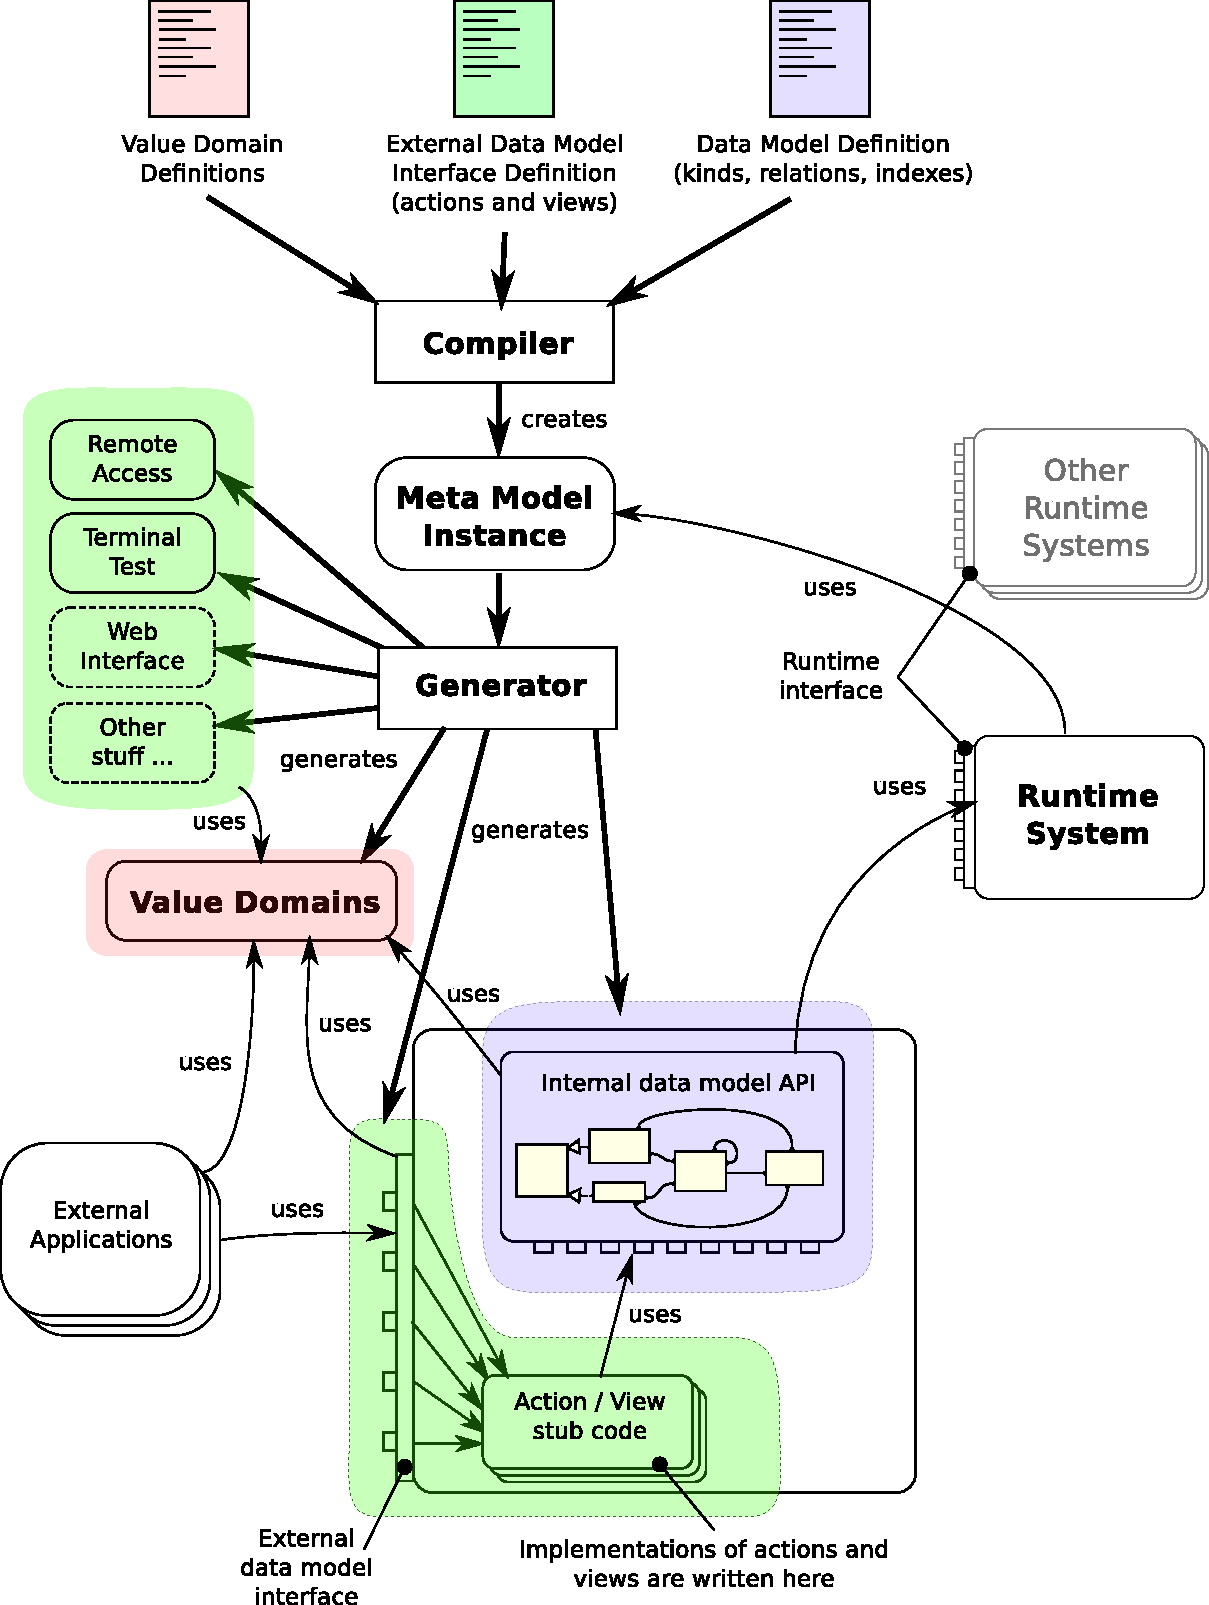
\includegraphics[width=\textwidth]{img/tobiasBilledeAfEdma.pdf}
\caption{Overview of the EDMA system. Definitions of value domains, data model external interface and data model structure are compiled into an instance of the meta model. The generator takes the meta model instance and generates model specific code including: Value domains, external data model interface and stub classes for implementing the methods in the external interface, an internal data model API that binds to the runtime system and various utility programs specialized to operate on the specific data model.}
\label{fig:tobiasBilledeAfEdma}
\end{figure}
\clearpage

We have taken an object oriented approach where the data model can
be seen as a class where the structure of the data model is encapsulated
from the outside world. The external interface of the data model is
the public part that external applications can use. As with classes
in object oriented languages, there can be several independent instances
of the same data model.

Each method in the external interface represents a transaction on
the data model. The semantic of the external interface is as if each
of these methods where synchronized on the same object. The individual
runtime system implementations may use more clever algorithms for
concurrency control, as long as the illusion of complete mutual exclusion
is kept intact. This analogy is used in order to keep focus on the
object oriented approach, instead of a traditional database approach.

The methods of the external interface are divided in two groups, \emph{views}
and \emph{actions}. Views cannot change the state of the data model
instance, only read it (this resembles const methods in C++). Actions
can both read and change the state of the instance.

In the following, we will describe the four main components in further
detail, starting with the meta model -- a very central element in
the EDMA system. Thereafter, we describe the compiler and the generator,
followed by a description of the example runtime system.


\subsection{\label{sub:Value-domains}Value Domains}

In most relational database systems, many different types of values
share the same data type. A person's name, an e-mail address, and
a URL could all have the same data type, e.g. \texttt{VARCHAR}. This
means that the type system is coarse grained, and it doesn't hinder
the user in storing, for example an e-mail, as a person's name.

In EDMA, we want to create a fine grained type system, where for example
an e-mail address, and a person's name belong to different types.
We call these types \emph{value domains}\nomenclature[value domain]{Value domain}{Can be seen as a type with extra restrictions on the possible values. Like the value 42 could be of type "int", the value "John" could be in a value domain "Name".}.

In EDMA we encourage the user to create a distinct value domain for
each semantically unique type. This not only adds useful semantic
information to the users of the value domains, it also makes the type
system able to discover a category of semantic errors, like if an
email address is accidentally used in place of a name or a URL.


\paragraph{Immutability}

In a multithreaded environment, mutable\nomenclature[mutable]{Mutable}{Changable. A mutable variable can get its value changed over the course of its lifetime.}
objects must be protected from race conditions, that can lead to threads
seeing them in an inconsistent state. For immutable\nomenclature[immutable]{Immutable}{Not changable. An immutable variable can never get its value changed over the course of its lifetime.}
objects this is not a problem, since they can never change after they
have been created. Therefore they will always be in a consistent state
(provided that they where created in a consistent state). Also, it
is never necessary to make defensive copies of immutable values, and
all values that are equal can be represented by the same instance.
For immutable values, the problem of accidental aliasing is also non-existing\cite{hogg1992geneva}.
For these reasons, in EDMA, all values (instances of value domains)
are immutable.


\paragraph{Value Domain Constraints}

The value domain system allows adding constraints to the value domains.
These constraints are automatically checked every time a new value
is created. As an example, the user can add a constraint to the value
domain \texttt{EmailAddress}, that checks that the content matches
a regular expression for accepted email addresses. 

There are two types of constraints on the value domains: \emph{Simple
constraints} and \emph{user implemented constraints}. The simple constraints
regard lengths and contents of strings, and numerical ranges for numeric
types. The user implemented constraints are, as the name suggests,
implemented by the user and can therefore be arbitrarily complex.

By defining constraints on the value domains the system can automatically
validate values when they are created.


\paragraph{Primitive Value Domains}

Value domains can be defined from the simple value domain types: \texttt{String},
\texttt{Integer}, \texttt{Long}, \texttt{Float}, \texttt{Double},
\texttt{Boolean} and \texttt{Enum}. Since we encourage the user to
create a fine-grained set of semantically unique value domains, the
primitive types can not be used directly, only in the definition of
other value domains.


\paragraph{Composed Value Domains}

It is possible to construct more complex value domains from the simpler
ones. For this purpose we have 3 different composable value domain
types: \texttt{Struct}, \texttt{List} and \texttt{OneOf}.


\paragraph{Struct}

The \texttt{Struct} value domain type consists of a number of attributes,
each of which has a name and a value domain. The struct value domain
type can therefore be seen as a container of multiple values, each
given a name. An example of a struct value domain, could be a \texttt{Date},
containing a \texttt{Day}, a \texttt{Month} and a \texttt{Year}. The
attributes in a struct value domain can be declared optional, which
means that the value might be \emph{null}.


\paragraph{List}

A \texttt{List} value domain type contains a number of values from
another value domain. For example, a value domain \texttt{NameList}
could be a list of \texttt{Name}s.


\paragraph{OneOf}

A \texttt{OneOf} value domain type contains a value from one of a
predefined set of value domains. An example could be a value domain
\texttt{Pet}, which can hold the value of either a \texttt{Dog}, \texttt{Cat},
or \texttt{Fish}. Thus the OneOf value domain type adds polymorphism
to the value domain system. 


\paragraph{Structurally Recursive Value Domains}

Value domains can be structurally recursive, meaning that for example
a value domain \texttt{Person} could contain a friend list of \texttt{Person}
values. But values (instances of value domains) are always tree-structures
and cannot contain loops or recursive references. In the above example
a person value cannot be in its own friend list. This is enforced
by the immutability of the values. It is only possible to construct
values from already created values, so all values are tree-structures
that are constructed in a bottom-up process. This means that it is
possible to define value domains where it would never be possible
to create a value from that value domain. 

An example would be a Struct value domain \emph{A} that contains a
field \emph{b} from value domain \emph{B} where the \emph{B} value
domain is a Struct containing a field \emph{a} from value domain \emph{A}.
You would need a value from value domain \emph{B} to create a value
from value domain \emph{A}, but to create a value from value domain
\emph{B} you need a value from value domain \emph{A}. One way to solve
this deadlock is to make at least one of the fields \emph{a} or \emph{b}
optional. The EDMA compiler will detect impossible value domains and
complain about them. This is done by checking that all recursive paths
contains an optional field, a list that may be empty or a OneOf with
a choice that breaks the loop.

There are advantages in having values that are guaranteed to be tree
structures and therefore self-contained and loop-free. This makes
processing values much simpler and the risk of entering an infinite
loop while processing values is greatly reduced. This also makes it
simple to move values across different borders of JVMs, machines,
languages etc.

It is worth to notice here that it \emph{is} possible to create a
value domain that represents a general graph by using indexes into
lists as references. However as long as the value domain contains
both the indexes and the lists they index into, this approach does
not break the self-contained and loop-free properties of the value
domain.


\paragraph{Expressiveness}

The value domain system is expressive enough to model itself as seen
in the following listing:

\begin{lstlisting}[basicstyle={\tiny},breaklines=true,tabsize=2]
ValueDomain MetaValueDomainSystem :
	List<MetaValueDomain> Constraints[noDuplicateOrMissingOrImpossible]
ValueDomain MetaValueDomain :
	Struct {name : UIdentifier, type : MetaValueDomainType, constraintList : ConstraintList}
ValueDomain MetaValueDomainType:
	OneOf<MetaPrimitiveType, MetaStructType, MetaListType, MetaOneOfType>
ValueDomain MetaPrimitiveType :
	OneOf<MetaStringType, MetaIntegerType, MetaFloatType, MetaBooleanType, MetaEnumType>
ValueDomain MetaStructType :
	List<MetaAttribute> Constraints[uniqueAttNames]
ValueDomain MetaAttribute :
	Struct {attName : LIdentifier, attValueDomain : UIdentifier, isOptional : TrueFalse}
ValueDomain MetaListType :
	Struct {elementValueDomain : UIdentifier, minLength : NotNegInt, maxLength : NotNegInt} Constraints[listMinLTEMax]
ValueDomain MetaOneOfType : List<UIdentifier>[1..MAX]
ValueDomain MetaStringType :
	Struct {minLength : NotNegInt, maxLength : NotNegInt, regexp? : Regexp} Constraints[stringMinLTEMax]
ValueDomain MetaIntegerType :
	Struct {min : AnyInt, max : AnyInt} Constraints[integerMinLTEMax]
ValueDomain MetaFloatType :
	Struct {min : AnyFloat, max : AnyFloat} Constraints[floatMinLTEMax]
ValueDomain MetaBooleanType :
	Struct {restrictedValue? : TrueFalse}
ValueDomain MetaEnumType : List<UIdentifier>

ValueDomain LIdentifier : String[1..MAX]["[a-z][A-Za-z0-9]*"]
ValueDomain UIdentifier : String[1..MAX]["[A-Z][A-Za-z0-9]*"]
ValueDomain TrueFalse : Boolean
ValueDomain AnyInt : Integer[MIN..MAX]
ValueDomain NotNegInt : Integer[0..MAX]
ValueDomain AnyFloat : Float[MIN..MAX]
ValueDomain Regexp : String[0..MAX]
ValueDomain ConstraintList : List<LIdentifier>
\end{lstlisting}


This makes it possible to create a value that represents a value domain
system for a specific domain, and use it as any other value in the
system e.g. use it in kind attributes, move it across socket connections
etc. It is also possible to model the meta model in the value domain
system, in this way an entire data model instance can be stored as
a single value.


\subsection{\label{sec:MetaModel}Meta Model}

The EDMA meta model is the central model that everything else in EDMA
is built around. The meta model is used to describe the individual
data models. An instance of the meta model represents a specific user
defined data model.

Since the meta model has many different elements, it is described
in a bottom-up fashion, starting with the most low-level definitions
first, gradually adding complexity as we go along.

%\begin{figure}[h]
%	\centering
%	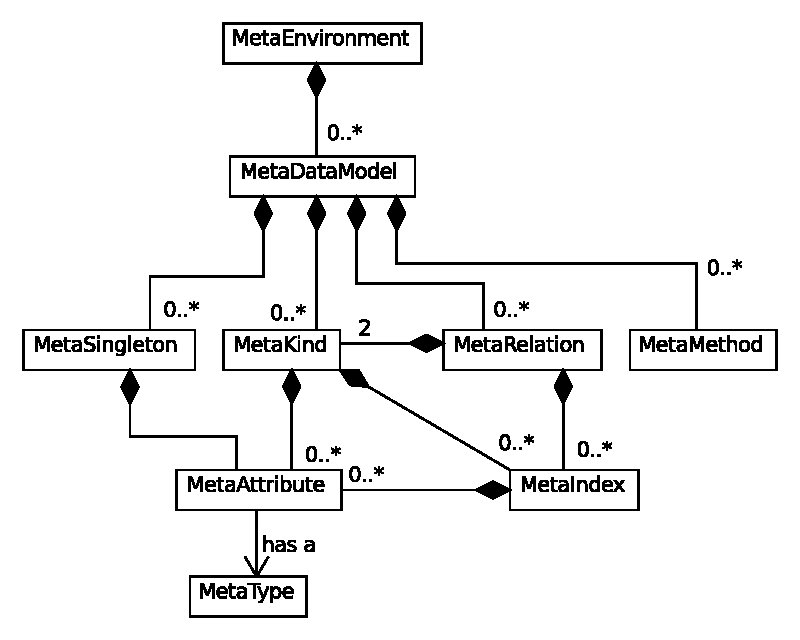
\includegraphics[width=0.75\textwidth]{img/metaModel.pdf}
%	\caption{The class diagram of the meta model is the %abstract syntax of the data model definition.}
%	\label{fig:metaModel}
%\end{figure}


\subsubsection{Kinds and Entities}

\begin{wrapfigure}{r}{0.4\textwidth}

	\begin{center}
		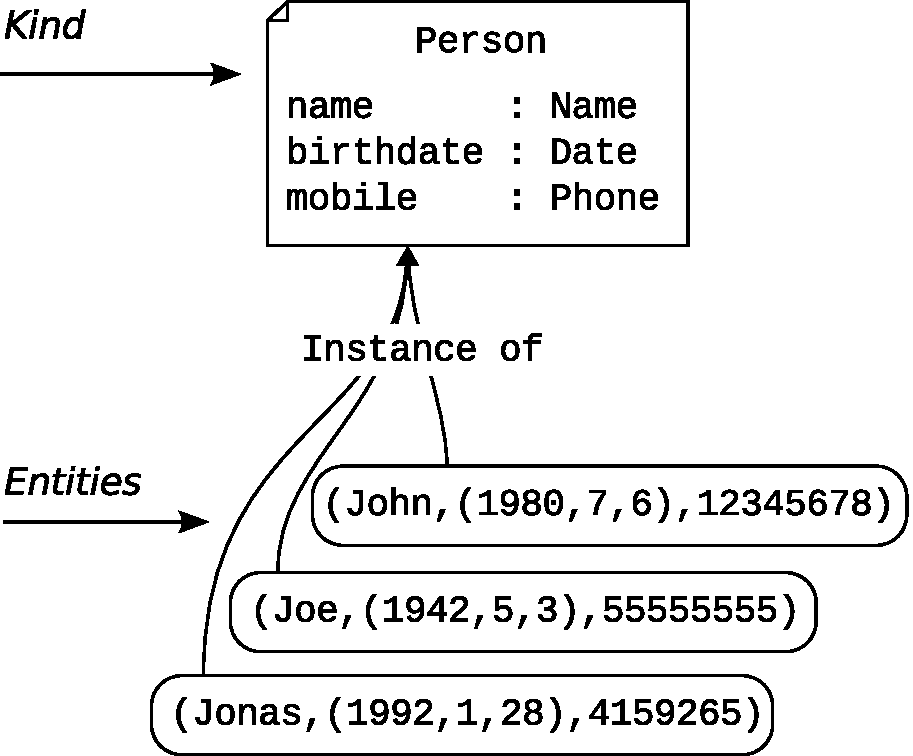
\includegraphics[width=0.4\textwidth]{img/kindAndEntities.pdf}
	\end{center}
	\caption{Kinds describe and contain entities, having certain attributes.}
	\label{fig:kindAndEntities}
\end{wrapfigure}

In EDMA a \emph{kind} \nomenclature[kind]{Kind}{A kind consists of a name and a set of attributes. An instance of a kind is called an entity. For example, a kind could be Person, with the attributes name, birth date and phone number. An entity of this kind could be (John, (1980, 3, 5), 31415926).}is
both a data type and a container of all instances of that type. A
kind has a set of \emph{attributes}\nomenclature[attribute]{Attribute}{A name and a value domain. An example could be "age" in the value domain "PositiveInteger", which is comparable to a variable "age" of type "uint". Attributes are either optional or mandatory, and mutable or immutable.},
where each attribute has a name and a value domain. An \emph{entity\nomenclature[entity]{Entity}{A set of values, conforming to a certain kind. }}
is an instance of a kind. As an example we could have a person kind
with attributes like name, gender, birth date, email and phone number.
A person entity would then contain a value for each of the attributes
in the person kind. Each attribute in a kind can be either mutable
or immutable. If it is immutable then a value for the attribute is
set upon creation of an entity, but this value can never change throughout
the lifetime of the entity. An attribute can be optional, which means
that the value corresponding to that attribute may be \emph{null}.
All kinds in EDMA have an attribute called ID, which is a positive
integer that uniquely identifies each \emph{entity} in the kind.


\subsubsection{Relations and Connections}

Assume that we have a person kind and a course kind, and we want to
be able to express that a person is a student on a course. In EDMA
we call this a \emph{relation\nomenclature[relation]{Relation}{A connection between two kinds. If a relation exists between kinds A and B, entities of A and B can be connected. For example, a relation can exist between kinds Course and Student, which means that an entity of course (eg. (Programming, 2012)) can be connected to a Student (eg. (John Doe, 1984, +4531415926)).}}
between the person kind and the course kind. When there is a \emph{relation}
between the person kind and the course kind, it is possible to make
a \emph{connection} between a specific person entity and a specific
course entity. A \emph{relation} is both a description of possible
\emph{connections} between entities and a container for these \emph{connections}.

\begin{figure}[h]
	\centering
	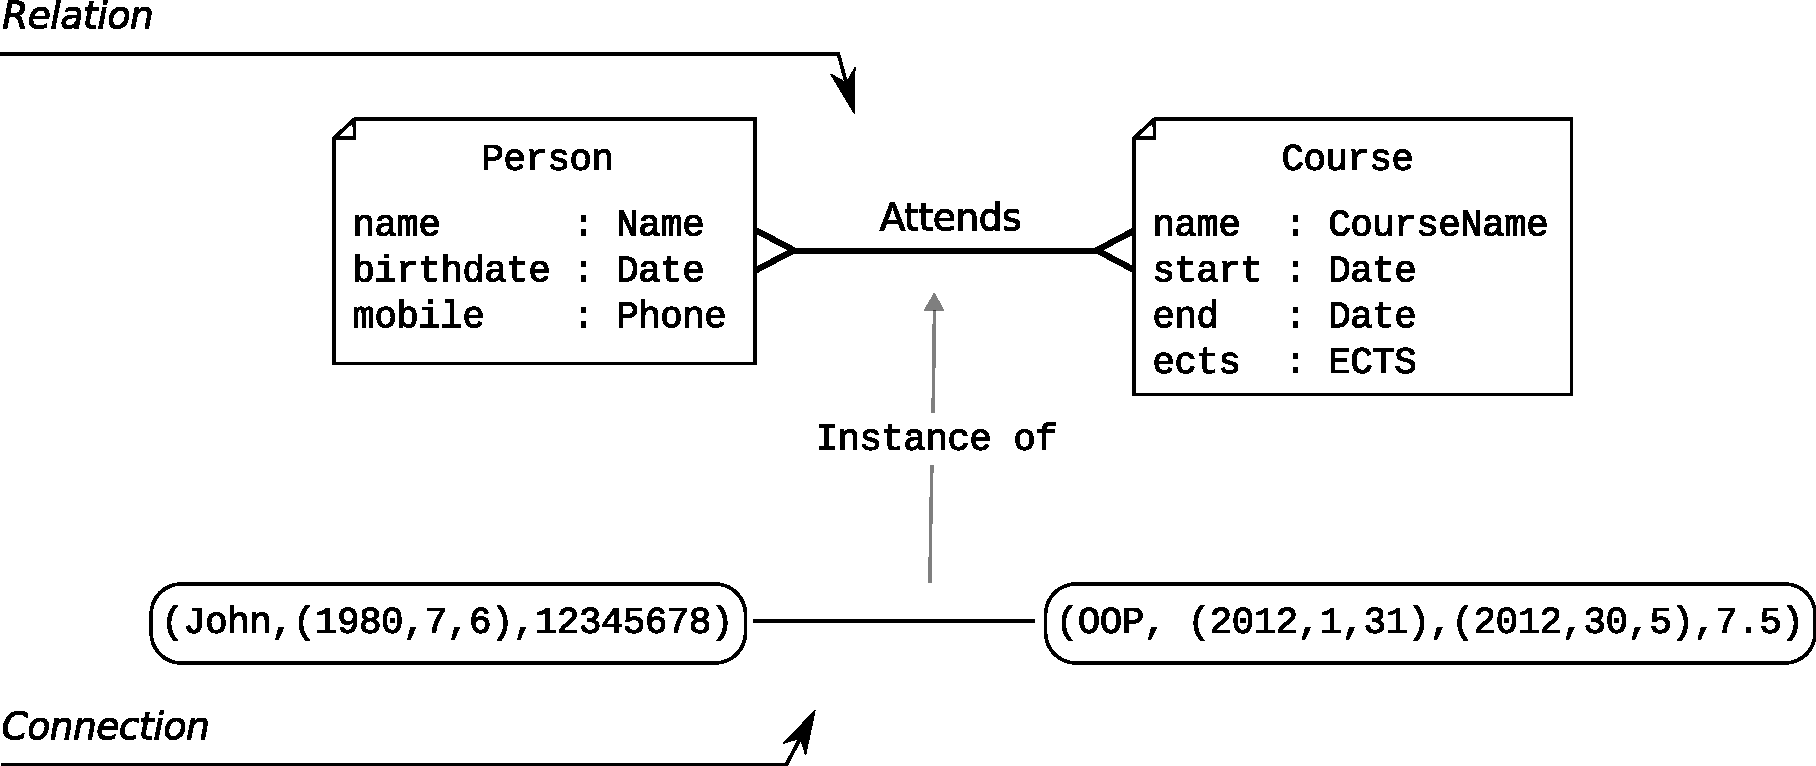
\includegraphics[scale=0.4]{img/relationAndConnection.pdf}
	\caption{A relation between two kinds makes it possible to \emph{connect} entities of those kinds.}
	\label{fig:relationAndConnection}
\end{figure}


\subparagraph{Roles}

A \emph{relation} always has two participants, which we can call A
and B. Both A and B are defined by a \emph{kind} and a \emph{role}.
The reason for having roles is that we can have different relations,
which involve the same kinds, in which case we use the roles to distinguish
them. In the example with the Person kind and the Course kind, we
could have two different relations between them: One that represents
students that are enrolled on the course, and one that represents
teachers that teach the course. To distinguish the two different \emph{relations},
the role of the person would be \emph{student} in the one relation,
and \emph{teacher} in the other. 

\begin{figure}[h]
	\centering
	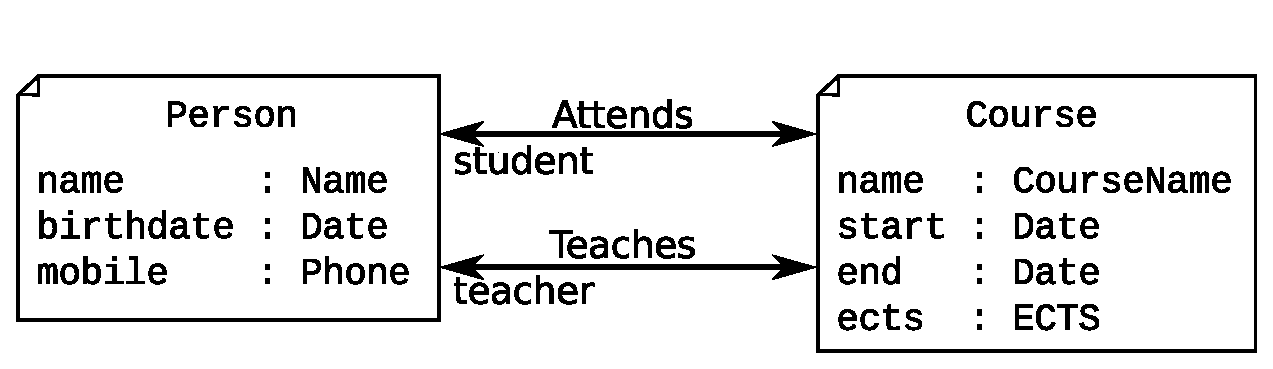
\includegraphics[width=0.75\textwidth]{img/relationRoles.pdf}
	\caption{A Relations between kinds can have roles. This figure shows two relations between the kinds Person and Course. In the first relation, named Attends, the first participant is the Person kind, with the role Student. In the second relation, Teaches, the Person has the role Teacher. In both Relations the second participant is the Course kind with the implicit role course.}
	\label{fig:relationRoles}
\end{figure}

It is also possible to have relations, where both the kind and the
role would be the same for A and B. An example could be a friendship
relation, where the kind is person and the role is friend for both
A and B, this type of relation we call a self-relation. If we have
a relation where A and B has the same kind, but different roles, then
it is not a self relation. An example of this could be where A and
B both are persons, but where the role of A is parent and the role
of B is child. In a self-relation, the order of the participants are
irrelevant, so if we have person a and person b, then ``a is friends
with b'' is the same as ``b is friends with a'', but there is a
difference between ``a is parent of b'' (or ``b is child of a'')
and ``b is parent of a'' (or ``a is child of b'').


\subparagraph{Multiplicities}

We also distinguish between many-to-many, many-to-one and one-to-one
relations (we do not have a one-to-many relation as this is the same
as a many-to-one where A and B are switched). It is worth to notice
that a many-to-one self-relation does not make any sense, so this
leaves us with five different types of relations:
\begin{enumerate}
\item Many-To-Many (MTM)
\item Many-To-Many-Self (MTMS)
\item Many-To-One (MTO)
\item One-To-One (OTO)
\item One-To-One-Self (OTOS)
\end{enumerate}
So, a relation in EDMA contains the following information: a name,
the kind of A, the role of A, the kind of B, the role of B, the type
of the relation (one of the five types above). If a role is not defined
on one of the participants, the role is set to the same as the name
of the participating kind. For example, in the relations shown on
Figure~\ref{fig:relationRoles}, the role of the Course is simply
``course''. In the five relation types above, \emph{many} actually
means \emph{0 or more} and \emph{one} actually means \emph{0 or 1}.

A \emph{connection} is an instance of a relation and can be thought
of as a set of pairs of ids (a, b). Each element in the set represents
the connection between an entity from kind A and an entity from kind
B with the ids a and b respectively. In a self-relation (a, b) is
the same as (b, a).


\subparagraph{Extension}

\begin{wrapfigure}{r}{0.3\textwidth}
	\vspace{-0.415cm}
	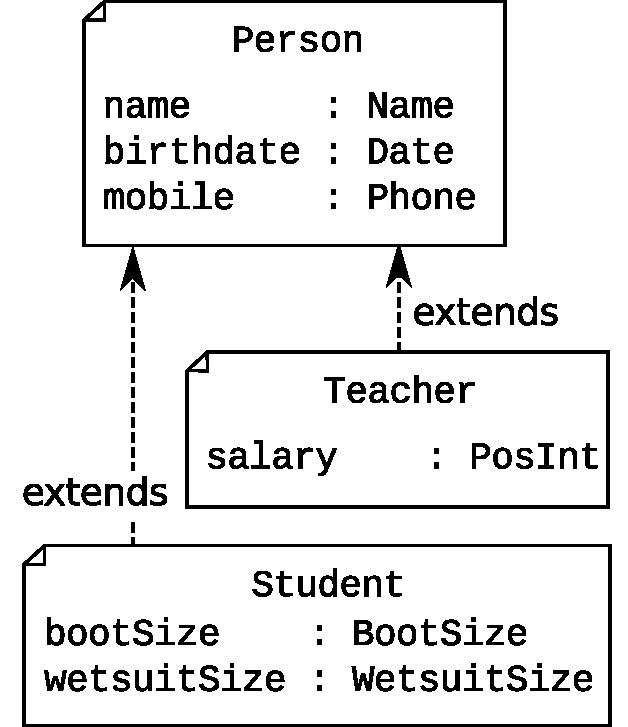
\includegraphics[width=0.3\textwidth]{img/kindExtension.pdf}
	\caption{Here, Student and Teacher extends Person, adding extra attributes.}
\end{wrapfigure}

There is actually a sixth relation type, which we call \emph{extension}.
An extension between kinds is a 1-to-(0 or 1) relation between two
different kinds. As an example we could have a kind, Person, and another
kind, Student, which extends Person. This means that every student
is also a person, so in order to create a new student, you would need
to provide an already existing person, that is not already a student.
We could also have another kind, Teacher, that also extends Person.
Then every teacher would also be a person, and a person could be both
a teacher and a student, or only one of them, or neither. In our running
example with the diving school, we have shown the kinds Student and
Teacher that both extend the kind Person.


\subsubsection{Indexes}

In EDMA indexes are used for two different purposes: To enforce uniqueness
of certain attributes within all entities of a kind, and to gain fast
and easy access to certain entities, or sets of entities. Indexes
can either be declared on a kind, in which case they cover all entities
of that kind, or they can be declared on a relation, in which case
they cover only sets of entities, that are grouped by that relation.
EDMA supports three types of indexes: \emph{Unique}, \emph{Equal}
and \emph{Compare}. 


\subparagraph{Unique index}

The \emph{unique index} is used to enforce uniqueness of one attribute
or a combination of attributes within all entities of a kind, or within
sets of entities grouped by a relation. The unique index also gives
a fast search mechanism using the attributes in the index. 

As an example, we could have a Person kind with attributes \texttt{firstName}
and \texttt{lastName}. If we declared a \emph{unique} index on (\texttt{firstName},
\texttt{lastName}) in the person kind, then this would enforce the
uniqueness of the combination of first name and last name, across
all person entities. If we were to create a person with a name that
were already taken, we would get an exception. If instead we declared
the index on a relation that connects persons and courses, then we
could have two or more persons with the same name, but they could
not attend the same course, because the index would cover every set
of persons connected to the same course.

In the example with the unique index on first name and last name,
it is very fast to get access to a specific person entity, given that
you know the first name and last name.


\subparagraph{Equals index}

The \emph{equal index} does not enforce any constraints, but are used
to get fast access to sets of entities, where the involved attributes
are equal to a certain value. As an example we could have an equal
index on the attribute \texttt{firstName}, making it very fast to
find all entities with a specific first name.


\subparagraph{Compare index}

Like the equal index, the\emph{ compare index} does not enforce any
constraints, but are only used to speed up certain searches among
entities. With a compare index, it is not only possible to search
for entities where the involved attributes are equal to some value.
It is also possible to find sets of entities, where the involved attributes
are less than a given value, greater than a given value or within
a range. The compare index uses the natural order of the value domains.


\subsubsection{Singletons}

Singletons are very similar to kinds, except that they contain exactly
one entity. If a singleton defines non-optional attributes, the values
for these attributes most be provided upon creation of the data model
instance. It is worth to note here that singletons are singletons
on the data model \emph{instance} level, not on the data model level.


\subsubsection{Actions and Views}

Kinds and relations make up the structure of the data model. Actions
and views make up the external interface to the data model. Actions
can both read and change the state of the data model instances, views
can only read the state. We call both actions and views \emph{methods}
if we do not need to distinguish between them.

Methods have a set of input and output parameters, each having a name
and a value domain. Both input parameters and output parameters can
be declared optional. Methods also return an error-code. The possible
error-codes are defined in the definition of the method. An error-code
of 0 always means that the method completed successfully and the output
parameters are valid. Any other error-code means that the method could
not complete for some reason and the output parameters are invalid
(meaning that they are all \emph{null}). For actions an error-code
different from 0 also means that the state of the data model is left
unchanged (any changes made by the action before it returns a non-zero
error-code is automatically rolled back).

An example of an action could be one for adding a student to a course.
It would take two input parameters: the ID of the student, and the
ID of the course, and the action would not have any output parameters
except for the error-code. Error-codes would then be defined for situations
where there is no student with the given ID, no course with the given
ID or the student is already assigned to the course. There could also
be an error-code for the situation where the student do not have enough
funding to pay for the course. As seen here the error-codes are dependent
on the business logic for the data model and the user can define any
number of error-codes that seems fit.

An example of a view could be getting the set of all students enrolled
on a specific course. This view would take a course ID as input and
the output would be a list of students. An error-code could be defined
for the situation where there are no course with the given ID.

The actions and views are atomic operations -- they either complete
successfully and return an error-code of zero, or they fail and return
a non-zero error-code, in which case no changes are made to the state
of the data model instance.


\paragraph{\label{sub:Transactions}Transactions}

Although we have taken an object oriented approach on the data models
and on a high level of abstraction see a data model instance as just
an object with synchronized methods, we want to elaborate a bit more
on the transactional model behind the scene.

In this subsection we will now switch to a more database oriented
terminology and call the methods on a data model instance \emph{transactions}.

The illusion of complete mutual exclusive access to a data model instance,
in database terminology, is the isolation property of the ACID (Atomicity,
Consistency, Isolation and Durability) properties.

Although some object oriented languages supports methods to obtain
isolation in multi-threaded environments, like the synchronize keyword
in Java, they do not incorporate support for the other ACID properties
in the core language.

This is something that we want to address in EDMA, therefore we will
now go through each of the ACID properties and discuss how they will
be handled in the example runtime. 


\subparagraph{Atomicity}

This guarantees that a transaction is executed as an atomic unit,
which means that it either completes successfully or does not change
the state of the data model at all. This property is only relevant
for \emph{actions}, since \emph{views} can never change the state
of the data model anyway. The way this is implemented is through a
rollback functionality. At any stage during the execution of an \emph{action},
if something unexpected happens, or if the action is not able to complete
successful for some reason, it can choose to abort (by returning a
non-zero error-code) and any changes it have already made to the state
of the data model up to this point will be automatically rolled back.

This has been implemented in the example runtime implementation by
defining a small set of six primitive reversible operations that can
be performed on the data model. These are the only operations allowed
on the lowest level, so every execution of an action are broken down
to a sequence of these primitive operations. When an action is executed
these primitive operations are recorded and in the case of a rollback
they can be inverted and played back in a reversed order which will
effectively bring the data model back to the starting state. The set
of primitive operations contains the following six operations:
\begin{itemize}
\item Update an attribute in a singleton
\item Create a new entity
\item Delete an entity
\item Update an entity
\item Create a new connection in a relationship
\item Delete an existing connection in a relationship
\end{itemize}
Each of these operations contains just enough information to be able
to perform the reversed operation as well. This means that ``updates''
contains both the old and the new values and ``deletes'' contains
information about the deleted item so it can be re-created. These
sequences of primitive operations are also the basis for the persistence,
which will be discussed later.


\subparagraph{Consistency}

When we say that the data model is in a consistent state, we mean
that all consistency rules set up by the designer of the data model
is respected in this state. Every \emph{action} must guarantee that
if it starts its execution with the data model in a consistent state,
then the data model is also in a consistent state upon successful
completion of the \emph{action. During }the execution of the action,
it is allowed for the data model to be in a non-consistent state.
In EDMA it is therefore considered as an \emph{error} in the programming
of an \emph{action} if it can move the data model from a consistent
state to a non-consistent state.

At the time of writing this document there have not been incorporated
a way to define consistency rules for EDMA data models (except for
the value domain system and the unique index). But this would be an
obvious extension of EDMA.

Depending on number and type of consistency rules it can be very slow
to test the consistency of a data model. Therefore it can be a good
idea to split consistency checks into different categories of checks
that only looks at parts of the data model. For example we could define
a kind consistency to only concern the attributes of an entity kind.
This consistency would only have to be checked when a new entity is
created or an existing entity is updated. Then we could define a relationship
consistency that would concern a specific relationship, this would
then have to be checked whenever a new connection is made, a connection
is removed or if any of the participating entities are updated. But
there could also be more complex consistency rules that would have
to look at larger parts of the data model and these would be difficult
to generalize about and therefore they would have to be checked after
each update of the data model. Because of the potential large impact
that consistency checks can have on the performance, we would consider
them as part of a debugging process and there should be a possibility
to turn them off when there is enough confidence in the implementations
of the actions and better performance is needed. 

It would be quite easy to implement a complete consistency check that
could be run after each successfully executed action, but we think
that a more general consistency and trigger framework is much more
desirable and therefore we have hesitated to implement this simple
solution.


\subparagraph{Isolation}

The isolation property says that during the execution of a transaction,
this transaction may not see any changes to the state of the data
model caused by other transactions. Or in other words: during the
execution of a transaction it must seem to that transaction that it
is the only transaction running at that time.


\subparagraph{Durability}

Traditionally durability means that once a transaction is committed
it stays so, even in the event of a system failure. As we see it,
there are at least two problems with this formulation:
\begin{enumerate}
\item It is not clear what is covered by the term ``system failure''.
Is it enough that data is stored on the local hard drive or should
it be stored on several different hard drives located in different
cities or even on different continents? No matter how secure the data
is stored it is always possible to think of some (maybe very unlikely)
event that would wipe out all the data. In the EDMA example runtime
implementation we have solved this by having an interchangeable persistence
module with a simple interface that handles the persistence strategy.
So in EDMA we define data to be persisted whenever the persistence
module say so.
\item It is not perfectly clear if this formulation covers both updates
and queries on the database. For \emph{actions} it is clear that when
they return from execution successfully, then any changes they have
made to the state of the data model should already be persisted. But
we think that it should also cover \emph{views}, so whenever a view
returns from execution, then any data seen by that view must be persisted.
\end{enumerate}
So in EDMA we will reformulate the durability property to something
that is a bit more clear on what we mean exactly: 

Durability is the property ensuring that: When a transaction (both
views and actions) has returned successfully from its execution, the
state of the data model known by the transaction at the end of the
execution, must be persisted successfully.


\subparagraph{Transaction Model}

Since we want to abstract a data model instance to an object with
synchronized methods that operates on an internal state, we have chosen
a flat transaction model, where the transaction begins upon entering
the method execution and ends upon exiting the method execution. In
this way the end user of EDMA will never have to think about transactions
or write transaction begin and end declarations.


\subsubsection{Data Models}

A data model can be seen as a class with an internal, encapsulated
state and an external interface. There can be many instances of the
same data model, just as there can be many instances of a class. A
data model instance also defines a transactional context, meaning
that the internal state of the instance is under transactional control,
but it is not possible to make transactions that span more than one
data model instance.

In a large software project there could be several different data
models covering different areas of the business model and there could
be several instances of each data model. 

The value domain system is the infrastructure that EDMA provides to
transport information between different data model instances. Since
all values in the value domain system are immutable and self-contained
it is easy to seamlessly distribute the data model instances on different
physical machines.


\subsubsection{Environment}

An environment is a collection of data models that ``speak the same
language''. By this we mean that the environment defines a set of
common value domains that the data models use in their methods. Each
data model can also define local value domains that are only relevant
in dealing with that specific data model.

Both the common value domains and the local value domains are available
to applications that uses the data models in the environment.



\subsection{EDMA Data Definition Language\label{sec:DataDefLanguage}}

In designing the syntax for the EDMA language, we have striven to
create a comfortable and easily learned language, for data and interface
definition. In this section we describe the textual syntax through
of the language through the use of examples. The complete EBNF grammar
is found in Appendix \ref{sec:EDMALanguageGrammar}.

The EDMA language is used to define both data and interfaces, using
the following structure:
\begin{itemize}
\item Value Domains (global value domains)
\item Data Models

\begin{itemize}
\item Local Value Domains
\item Singletons
\item Kinds
\item Relations
\item Actions
\item Views
\end{itemize}
\end{itemize}
Since value domains can be shared by several data models, they can
be defined outside the context of data models. Data models are defined
with a block-structure (delimited by curly brackets), containing local
value domains, singletons, kinds, relations, actions and views inside
the block. White spaces and newline-characters are ignored, meaning
that blocks can be written on a single line.

It is possible to divide the definition into different files. For
example, the user might want to have all the global value domains
in one file, kinds, relations and singletons in a second file, and
actions and views in a third file. 

The syntax makes use of a set of reserved keywords, partly to make
the language easy to read and understand for the user, partly to make
it easier to parse. In the following, examples of each element type
are used to explain the syntax.


\paragraph{Value Domains}

Value domains are defined by a keyword \textbf{ValueDomain} followed
by an identifier, the name of the value domain. The name of the value
domain is written in camel case, and may contain numbers, although
the first character of a value domain name must be an uppercase letter.
After the identifier, a colon is written, followed by a type of primitive.
There are 9 types of primitives, represented by the following keywords:
\textbf{Integer}, \textbf{Long}, \textbf{Boolean}, \textbf{Float},
\textbf{Double}, \textbf{Struct}, \textbf{Enum}, \textbf{OneOf} and
\textbf{List}. The colon serves to represent a type declaration, and
can be read as ``of type''. After the primitive type has been given,
the user can optionally declare a constraint on the value domain.
An example of a value domain declaration is shown in the following
listing. 

\begin{lstlisting}[language=edma]
ValueDomain Month : Integer[1..12]
\end{lstlisting}

In the example given, the Month value domain is constrained to be
in the range 1 to 12, both inclusive. For the number types, the constraint
is always considering the range of values. The constraint is written
in the form \texttt{{[}a..b{]}}, where \texttt{a} and \texttt{b} are
numbers, and where \texttt{b} $\geq$ \texttt{a}. Alternatively, the
user can use the keywords \textbf{MIN} and \textbf{MAX} to represent
the smallest or largest possible number. 

For the String primitive type, the constraint considers the length
of the string. The user can also specify a regular expression in a
quoted string between \textbf{{[}} and \textbf{{]}}. Values matching
the given regular expression are considered valid.

The \textbf{Long}, \textbf{Float} and \textbf{Double} value domains
are written in the same way as the Integer value domain, using the
respective keywords.

The List value domain is written with the contained value domain given
between a pair of angle brackets. Optionally, the user can declare
a length constraint on the list on the form \texttt{{[}a..b{]}}, as
the range constraint on number value domains. An example of a List
definition is shown in the following listing.

\begin{lstlisting}[language=edma]
ValueDomain StudentList : List< Student > [0..99]
\end{lstlisting}

The Enum value domain is written with the possible enumeration values
in square brackets, as shown in the example in the following listing.

\begin{lstlisting}[language=edma]
ValueDomain Animal : Enum[Cat, Dog, Horse]
\end{lstlisting}

Like the numerical constraint is written in square brackets, we can
see the enum values as being the constraint of the enum type, i.e.
the value of an Animal type must be one of the given enumeration types.

The OneOf value domain is defined almost like the Enum value domain,
but with angle brackets, as shown in the following example.

\begin{lstlisting}[language=edma]
ValueDomain Person : OneOf<Teacher, Pupil>
\end{lstlisting}

This bears resemblance to the notion of parametrized types in Java,
generics, which is written as for example \texttt{ArrayList<Point>}.

Structs are defined by declaring the primitive type \textbf{Struct},
followed by a block delimited by curly brackets. Inside the block
is written a comma separated list of attributes. The following example
shows the definition of a struct.

\begin{lstlisting}[language=edma]
ValueDomain Person : Struct
{
	name : Name,
	age? : PositiveInteger,
	phone : PhoneNumber
}
\end{lstlisting}

Each attribute consists of a name, a colon (again, to declare that
the type, or value domain, is following), and a value domain. Attributes
may be declared optional, by writing a question mark after the attribute
name. The attribute type must be a non-primitive value domain. 

Since white spaces are ignored, it is possible to write structs in
a more compact style, like shown in the following example.

\begin{lstlisting}[language=edma]
ValueDomain Date : Struct { y:Year, m:Month, d:Day }
\end{lstlisting}

Because the attributes are separated by comma, the compact style is
still readable. In contrast, the user can also add extra white space,
as to impose a structure to make it more readable. This is shown in
the following example.

\begin{lstlisting}[language=edma]
ValueDomain Person : Struct
{
	firstName : Name,
	lastName  : Name,
	age       : Age
}
\end{lstlisting}


\subparagraph{Custom Constraints}

The user can write custom constraints on value domains. Custom constraints
are implemented manually by the user (in generated stub-files), and
thus can be arbitrarily complex. The custom constraints are written
immediately after the value domain definition, starting with the keyword
\textbf{Constraints}, following a square bracket enclosed, comma separated
list of constraints. Each constraint is a camel case word with a lower-case
first character, and optionally, a double quoted string describing
the constraint. The following listing shown an example of a value
domain Date with constraints for disallowing non-work days.

\begin{lstlisting}[language=edma]
ValueDomain Date : Struct
{
	year : Year,
	month : Month,
	day : Day
} 
Constraints[leapYearCheck "Checks for leap year correctness",
 workDays "Checks that the date represents a work day"]
\end{lstlisting}

Another example of a custom constraint is shown in the following listing.
The example shows a definition of the value domain OddNumber with
a constraint declaration.

\begin{lstlisting}[language=edma]
ValueDomain OddNumber : Integer 
Constraints[oddNumber "Checks that the number is odd"]
\end{lstlisting}

As the user can omit the quoted descriptions, constraints can be written
in a more compact form, as shown in the following listing.

\begin{lstlisting}[language=edma]
ValueDomain WorkDate : Struct { y:Year,m:Month,d:Day }
Constraints[leapYear, notWeekend, notHoliday, notMothersDay]
\end{lstlisting}


\paragraph{Data Models}

Data models are defined using the keyword \textbf{DataModel}, followed
by an identifier making up the name of the data model. The name of
the data model must be written with a capital first letter, like the
name of value domains. After the name, a curly-bracket delimited block
follows, containing definitions of local value domains, singletons,
kinds, relations and actions and views. An example of an empty data
model is shown in the following listing.

\begin{lstlisting}[language=edma]
DataModel DivingSchool
{

}
\end{lstlisting}

Data model definitions can be split up into several blocks. In that
way, the user might create different parts of the data model in different
files. The following example shows one single data model, defined
over two files. Each of the two partial definitions of the single
model contains a local value domain definition. Thus, the DivingSchool
data model will contain two local value domains.

\begin{lstlisting}[language=edma]
DataModel DivingSchool
{
	ValueDomain WetsuitSize : Enum[XS, S, M, L, XL, XXL]
}
\end{lstlisting}
\hrule
\vspace{8pt}
\begin{lstlisting}[language=edma]
DataModel DivingSchool
{
	ValueDomain BootSize : Integer[25..48]
}
\end{lstlisting}


\paragraph{Kinds}

The definition of kinds follows the same style as the definition of
data models. First, the keyword \textbf{Kind} is given, followed by
the name of the kind. The name of the kind must start with a capital
letter. Like structs value domains, kinds have a comma separated list
of attributes. The following example shows a definition of a kind
inside a data model.

\begin{lstlisting}[language=edma]
DataModel DivingSchool
{
	Kind Person
	{
		firstName     : Name,
		middleName ?  : Name,
		lastName      : Name,
		phoneNumber + : Phone,
		email     ? + : Email
	}
}
\end{lstlisting}Like in structs, attributes can be declared optional by adding a question
mark after the name. Further more, attributes in kinds may be declared
mutable with a plus-sign after the name (this is not possible in value
domains, as they are immutable.)

When defining a kind, EDMA automatically defines a local value domain
resembling the entities of that kind. The local value domain corresponding
to the one generated from the previous listing, is shown in the following
listing.

\begin{lstlisting}[language=edma]
ValueDomain Person : Struct
{
	firstName    : Name,
	middleName ? : Name,
	lastName     : Name,
	phoneNumber  : Phone,
	email      ? : Email
}
\end{lstlisting}

In some cases, the user might want to make the generated local value
domain visible outside the data model. This can be done by declaring
the kind public, and optionally, declaring it public under a certain
name. This can be done with the \textbf{Publish} and \textbf{Publish
As} keywords respectively. If no name is given, the local value domain
will be published under its own name. In the following example, a
Person kind is published as DivingSchoolPerson (omitting the details.)

\begin{lstlisting}[language=edma]
Kind Person Publish As DivingSchoolPerson { ... }
\end{lstlisting}

Further more, a kind can extend another kind. Kind extension is declared
with the keyword \textbf{extends}, as shown in the following example
(omitting the details.)

\begin{lstlisting}[language=edma]
Kind Student extends Person { ... }
\end{lstlisting}

A kind can have indexes defined on any of its attributes, or list
of attributes. An index is declared on one or many attributes by writing
one of the three keywords, representing the three kinds of indexes,
\textbf{Unique}, \textbf{Compare} and \textbf{Equals}. The keyword
is followed by a comma separated list of attribute names, enclosed
in parenthesis. An example of a Person kind with a compare index is
shown in the following listing.

\begin{lstlisting}[language=edma]
Kind Person
{
	firstName : Name,
	lastName  : Name,
	Compare(firstName, lastName)
}
\end{lstlisting}

The index follows the natural order of the value domains.


\paragraph{Singletons}

Singletons are defined in the same style as kinds, but with the \textbf{Singleton}
keyword used instead of the \textbf{Kind} keyword.


\paragraph{Relations}

A relation is defined by its name, the type of relation, and the two
kinds that participate in the relation, and their roles. A relation
definition starts with the \textbf{Relation} keyword, followed by
the name of the relation. The relation name must start with a capital
letter. After the relation name comes the first relation participant,
the relation type, and the second participant. Each participant is
written as two colon-separated parts, the name of a kind, and the
lowercase role name. The user can leave out the colon and role, in
which case the role will be the same as the kind. An example of two
relation definitions are showed in the following listing.

\begin{lstlisting}[language=edma]
Relation StudentEnrolled Course >-< Person : student
Relation TeacherEnrolled Course >-- Person : teacher
\end{lstlisting}

The relation type is shown with the \texttt{\textbf{>-<}} symbol,
to mimic crows-feet notation. The three relation types available are
\texttt{\textbf{>-<}}, \texttt{\textbf{>-{}-}} and \texttt{\textbf{-{}-{}-}}.
The ``many'' part of a many-to-one or one-to-many relation is always
written on the left side.

Indexes can be defined on relations, as well as on indexes. When defined
on a relation, the user must choose on which of the participants the
index is placed, with the \textbf{On} keyword. The index declaration
is placed inside a block delimited by curly brackets. The following
example shows a relation with a unique index.

\begin{lstlisting}[language=edma]
Relation Enrollment Course >-< Person : student
{
	Unique On Person(firstName, lastName)
}
\end{lstlisting}

If the relation is between two of the same kinds, a colon and role
name can be supplied after the kind name.

Constraints can be declared on relations, by using the same syntax
as constraints in value domains. The constraints must be written inside
the block, where also the relation indexes are written.


\paragraph{Actions and Views}

Actions and views are defined inside a data model block, starting
with either of the keywords \textbf{Action} or \textbf{View}. The
syntax of actions and views are similar, besides the keyword. After
the keyword follows the name, which must start with a lowercase letter.
The name is followed by a block delimited by curly braces. Inside
the block, four keywords are recognized: \textbf{Input}, \textbf{Output},
\textbf{ErrorCodes} and \textbf{Description}. The input and output
declarations are followed by colon, and a comma separated list of
attributes, given either as inputs or outputs. An error code is written
as a number (the error code), a hyphen for separation, and quoted
error text. The description keyword lets the user write a quoted string,
acting as a description. The following example shows the definition
of a view and an action.

\begin{lstlisting}[language=edma]
Action createTeacher
{
	Description: "Create a new teacher from a person."
	Input: 
		personID : PersonID,
		salary : PosInt
	Output:
		id : TeacherID
	ErrorCodes:
		1 - "Person does not exist",
		2 - "Person is already a teacher"
}

View getCoursesFromStudent
{
	Description:
		"Returns a list of courses, 
		given a student id"
	Input:
		sid : StudentID
	Output:
		courses : CourseList
	ErrorCodes:
		1 - "Non-existing student"
	
}
\end{lstlisting}The input, output, description, and error code sections can be written
in any order.


\paragraph{Comments}

The syntax for comments is like that of Java, \textbf{//} denounces
a line comment, while \textbf{/{*}} and \textbf{{*}/} is used for
block-commenting.



\subsection{Compiler}

In this section, we describe the compilation of EDMA data definition
files. The compiler consists of three parts: a parser, a translator,
and a generator. An overview of the compilation process can be seen
on Figure~\ref{fig:compilation}.

\begin{figure}[h]
	\centering
	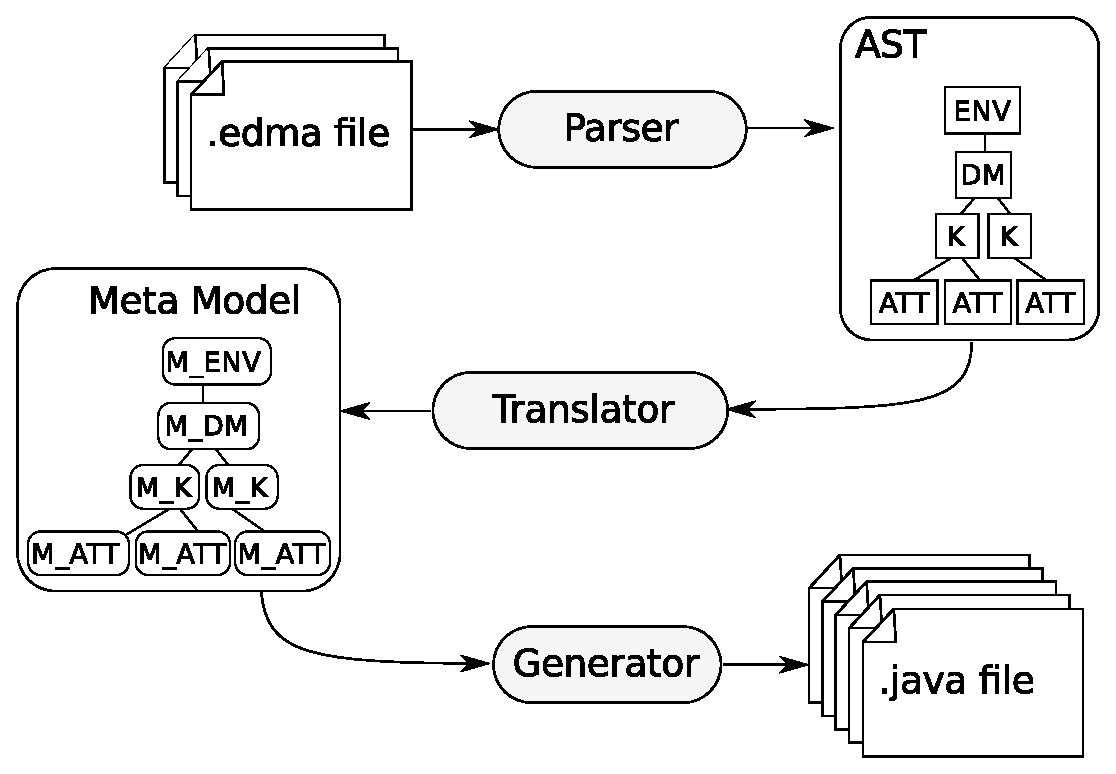
\includegraphics[scale=0.5]{img/compilation.pdf}
	\caption{The compilation of EDMA data definition files is done in three steps: parsing, compilation into a meta model, and generation of Java files.}
	\label{fig:compilation}
\end{figure}

A parser takes in one or many data model definition files with the
extension \texttt{.edma}. While parsing the files, an abstract syntax
tree (AST) representing the data models, is being created. The translator
translates the AST into a meta model, which can then be fed to the
generator. The generator is responsible for outputting Java classes
and interfaces, reflecting the user's data model definition.

It is worth noting, that the abstract syntax tree defines the logical
structure of our environment and data models. The important feature
of the AST is that it makes the translator completely independent
of the concrete textual syntax used in the EDMA language. Having the
AST makes it easy to change the textual grammar and create other syntaxes,
and even create other types of syntaxes. For example, it would be
possible to implement a graphical user interface for drawing data
models, thus serving as a syntax.


\subsubsection{Parser}

For defining the grammer of the textual syntax, we have used a parser
/ scanner generator known as JavaCC. From a JavaCC-grammer, a Java-based
top-down LL(k) parser is generated. The grammar specification is a
variation of EBNF, mixed with Java code for building an instance of
the AST.


\subsubsection{Translator}

The translator takes an AST representing the data model definition,
and creates a meta model instance. The meta model instance can be
seen as an internal representation of the data model definition, and
it is used by both the generator, and by the EDMA runtime system.

When the translator has got a complete AST from the parser, resembling
the user's data model, it does two things. First, it checks whether
everything is consistent within the AST. Then, it simply translates
the AST instance into a Meta Model instance.


\subparagraph{AST Consistency}

In the grammar, syntactical rules governing the data model definition
are specified. However, even if the language is only a data definition
language, there are also some semantic rules, that we must enforce.
Before translating the AST into a meta model, the translator checks
for the presence of circular extensions, unknown references, invalid
ranges in constraints, and value domain loops.
\begin{description}
\item [{Circular~Extensions}] -- The kinds Person and Student could be
defined to extend each other. Instantiation of either would require
an instance of the other to exist. Therefore, we prohibit the user
from making circular extensions of kinds.
\item [{Unknown~References}] -- Wherever the user has written a reference
to an attribute name or a kind name, it must be checked whether the
given attribute or kind is actually defined.
\item [{Value~Domain~Range~Checks}] -- Since the user can specify ranges
on numerical value domains, we have to check that the ranges supplied
actually make sense. For example having a minimum value that is greater
than the maximum value, should be invalid.
\item [{Value~Domain~Loops}] -- Having immutable value domains may be
tricky for the unaware user. Without any check for loops, the user
would be able to define value domains for which there could never
be a valid value. A value domain A of type Struct, could contain an
attribute b, of type \texttt{B}. Likewise, a value domain B of type
Struct could contain an attribute of type A. This is shown on the
listing below.\\
\begin{lstlisting}
ValueDomain A : Struct {
  b : B
}
ValueDomain B : Struct {
  a : A
}
\end{lstlisting}Since in A, b is not optional, it must be supplied at the instantiation
of A. Similarly, when creating a value of B, a value of A must be
supplied. The user could declare a type of B, and set it to null,
and feed it to A upon creation, but this will make the instantiation
of B fail with a nullpointer exception. Since the user might accidentially
create loops, by having many different inter-related value domains,
we have put a check into the compiler, to make it fail as early as
possible.
\end{description}
As soon as an error has been found in the AST, we print out the problem,
the file name and the line number where the error occurred. Each element
in the AST is created with the file name and line number of the statement,
that was the source of it's creation. Therefore, we can easily print
it out when an error occurs in the compilation stage.

After the meta model has been created, the compiler invokes the Generator,
which then starts generating the model-specific Java code.



\subsubsection{Generator\label{sec:Generator}}

The generator is the module responsible for generating Java classes
and interfaces for a specific instance of the meta model.

The generator generates the following:
\begin{itemize}
\item Interfaces and classes for each Value Domain defined in the environment
and the data models.
\item The environment class that contains the instance factories for each
data model in the environment.
\item An instance factory for each data model in the environment, that controls
the individual instances of the data model.
\end{itemize}
For each data model in the environment, the following is generated:
\begin{itemize}
\item The set of interfaces that makes up the internal API, used by the
actions and views to manipulate and view the state of the data model
instance.
\item The set of classes that implements the internal API and binds it to
the runtime interface.
\item The stub classes where the user implements the actions and view. There
is one stub class for each action and view.
\item The external interface for the data model.
\item The implementation of the external interface, that binds the methods
of the interface to the stub classes and execute them through the
runtime interface.
\end{itemize}

\subparagraph{}


\paragraph{\label{sub:Creation-of-values}Value Domains}

The value domains are the type system and infrastructure in EDMA that
binds everything together and ensures that every part of a project
speaks the same language. Each value domain represents a unique type
of data with a well defined structure.

The generator generates two classes for each defined value domain:
An abstract class that serves as an interface to values from the value
domain and an implementation class that implements the abstract methods
in the interface. The reason for using an abstract class instead of
a Java interface is that Java does not support static methods in interfaces
and there are several static methods used to create new values:
\begin{itemize}
\item create - this method creates a new value from scratch 
\item fromString - this method creates a new value from the string representation
of the value.
\item fromStream - this method reads a value from a stream.
\item fromStreamNoValidate - this method reads a value from a stream without
validating it. It should only be used when reading from a trusted
source. For large complex values with many constraints the validate
process could be slow, that is the reason for having this method.
\item fromTerminal - this method uses a terminal to instruct a user to create
a new value.
\end{itemize}
And some abstract methods:
\begin{itemize}
\item toString - returns the string representation of the value.
\item toStream - writes the value to a stream.
\end{itemize}
All value domain classes also have sensible implementations of the
comparable interface, the hashCode and equals methods.

The create method for struct type value domains uses a modified version
of the builder pattern to create new values. The builder pattern uses
what is known as a fluid interface\cite{fowler2008}, where methods
are chained together. This results in more readable code, where each
field has a set-method named after it. In EDMA we have taken the builder
pattern one step further, so each field has its own interface, with
a set-method named after the field. Each set-method then returns the
builder-interface for the next field except the last one, which returns
the created object or value. By doing it this way, we get a fixed
order of the attributes and we make sure that it is not possible to
miss out on any of them. It would be a bit cumbersome to program this
by hand, but with auto-generated code it is no problem. As an example,
lets see how we would create a new date from the date value domain:

\begin{lstlisting}[language=java,frame=none]
Date myDate = Date.create().year(1973).month(6).day(7);
\end{lstlisting}The static method \texttt{Date.create()} returns an interface that
only has a method for setting the year. That method returns an interface
with a method to set the month, which in turn returns an interface
to set the day. The interface for setting the day finally returns
the completed data value. If we put the attributes in a wrong order
or if we missed out any of them, then the Java compiler would complain
immediately. If the user uses a modern IDE e.g. eclipse, it gets very
easy since the automatic code-completion will pop up with the name
of the next field after each dot. This type of chained interfaces
are used in EDMA both when creating values from value domains and
when creating entities from kinds.


\paragraph{Data Models}

For each data model in the environment, several interfaces and classes
are created:
\begin{itemize}
\item Data model factory interface. This interface provides methods to create
new instances of the data model and to get access to existing instances
of the data model. Each instance is identified by a name.
\item Data model instance interface. This interface is used to start and
stop the instance and to get the external interface of the instance.
The methods of the external interface can only be called when the
instance is running. Otherwise an exception is thrown.
\item Data model external interface. This is the external interface of the
data model that clients can use to execute the actions and views on
the data model.
\item Internal view interface. This is the interface that \emph{views} use
internally to navigate and extract information from the data model.
\item Internal update interface. This interface extends the internal view
interface and adds functionality to make changes to the data model.
This is the interface that \emph{actions} use internally.
\end{itemize}
Besides these interfaces there are also generated classes that bind
these data model specific interfaces to the general runtime interface.


\paragraph{Kinds}

For each kind in the data model we create a number of interfaces that
can be used internally in the implementation of the views and actions.
These interfaces are:
\begin{itemize}
\item The entity view interface. This interface provides methods to read
the attributes of an entity of this kind. It will also get the methods
that are used to navigate any relations that this kind is part of.
\item The entity update interface. This interface extends the view interface
and adds methods to update the mutable attributes. This interface
will also get methods to create and delete connections with other
entities through the relations that this kind is part of.
\item The set interface. This interface is used to navigate sets of entities
of this kind. It implements the iterable interface and has methods
to create new sets by unions, intersections and subtractions with
other sets of the same kind. It also gets methods to navigate relations
that this kind is part of.
\item The filter interface. This is a simple interface that can be used
to create specialized filters that can be used on sets of entities
of this kind.
\item The kind interface. This interface has methods to get access to all
entities of this kind or a specific entity either by ID or by any
unique index on the kind. It also has methods to get access to specific
sets of entities based on the indexes declared on this kind.
\end{itemize}
For each kind in the data model, the internal view interface for the
data model gets a method to access the kind interface and the internal
update interface gets methods to create new entities and delete entities
of this kind and a method to upgrade a view interface for an entity
of this kind to an update interface. For singletons we only have the
entity view and entity update interface.

The way we update entities is a little special because of the unique
index. Normally we would just make a set method for each mutable attribute
and then these could be used to update entities one attribute at the
time, but this could give problems if there are unique indexes that
span more than one attribute. As an example, lets say we have a person
kind with separate attributes for first name and last name and that
we have a unique index on (firstName, lastName). There exist a person
called ``John Andersen'' and another person called ``Thomas Andersen''.
Lets say we want to change the name of ``Thomas Andersen'' to ``John
Nielsen'', then we would get an UniqueException if we started by
changing his first name to ``John'', because now there would be
two people named ``John Andersen''. To solve this we have made it
possible to update several attributes at once. Instead of doing something
like this:\begin{lstlisting}[language=java,frame=l]
person.setFirstName("John");
person.setLastName("Nielsen");
\end{lstlisting}We instead do like this:\begin{lstlisting}[language=java,frame=l]
person.setFirstName("John").setLastName("Nielsen").save();
\end{lstlisting}Thus, we update both the first name and the last name at the same
time and we will only get an UniqueException if there is another person
named ``John Nielsen''. The \emph{save} method only declares that
it can throw a UniqueException if we actually update an attribute
that is part of a unique index. This is done by a little trick, where
we actually have two different interfaces for updating the attributes,
a \emph{plain} one where the \emph{save} method does \emph{not} throw
a UniqueException and a \emph{unique} one where the \emph{save} method
declares to throw the UniqueException. In the \emph{plain} interface
all set methods on attributes that are not part of a unique index
just return the \emph{plain} interface again, but the set methods
for those attributes that are involved in a unique index returns the
\emph{unique} interface instead. In the \emph{unique} interface all
set methods returns the \emph{unique} interface again. So this does
that as soon as we have ``touched'' an attribute that is part of
a unique index, then the \emph{save} method will declare that it can
throw the UniqueException.

Besides these interfaces there are also generated classes that binds
these data model specific interfaces to the general runtime interface.


\paragraph{Relations}

The relations in the data model add methods to the interfaces for
the kinds participating in the relation. The names of these methods
are dependent on the type of the relation, as well as names and roles
of the participating kinds. For example, having a relation \texttt{StudentEnrollment}
between \texttt{Course} and \texttt{Person} (having the role of \texttt{student})
results in four methods; two in the \texttt{CourseUpdate} interface
(\texttt{addStudent} and \texttt{removeStudent}), one in the \texttt{PersonViewer}
interface (\texttt{asStudentGetCourseSet}) and one in the \texttt{CourseViewer}
interface (\texttt{getStudentSet}). This is visualized in figure~\ref{fig:generatorRelations}.

\begin{figure}[h]
\rule{\textwidth}{.1mm}
\emph{EDMA file:}
\begin{lstlisting}[language=edma,frame=l]
Relation StudentEnrollment Course >-< Person:student
\end{lstlisting}
\emph{Generated Java:}
\begin{lstlisting}[language=java,frame=l]
public interface CourseUpdater {
	boolean addStudent(PersonViewer student);
	boolean removeStudent(PersonViewer student);
	. . .
}
public interface PersonViewer {
	CourseSet asStudentGetCourseSet();
	. . .
}
public interface CourseViewer {
	PersonSet getStudentSet();
	. . .
}
\end{lstlisting}
\rule{\textwidth}{.1mm}
\caption{Top: The relation as represented in the data definition language. Bottom: The generated code.}
\label{fig:generatorRelations}
\end{figure}Notice that the method in the course viewer interface is not named
\texttt{asCourseGetStudentSet}, but just \texttt{getStudentSet.} Methods
in the \texttt{PersonUpdate} interface for adding and removing courses
(as a student) could be generated as well; however, these would be
redundant with the \texttt{addStudent} and \texttt{removeStudent}
in the \texttt{CourseUpdater} interface. Therefore, the generator
only creates connection methods on the first kind in the relation
(the kind written to the left in the relation declaration).

In a one-to-many relation, a method returning a set of the other kind,
is created on the first kind, while a method returning a single entity
is created on the second kind. This is shown in figure~\ref{fig:generatorRelationsManyOne}.

\begin{figure}[h]
\rule{\textwidth}{0.1mm}
\emph{EDMA file:}
\begin{lstlisting}[language=edma,frame=l]
Relation TeacherAssignment Course >-- Person:teacher
\end{lstlisting}
\emph{Generated Java:}
\begin{lstlisting}[language=java,frame=l]
public interface PersonViewer {
	CourseSet asTeacherGetCourseSet();
	. . .
}
public interface CourseViewer {
	PersonViewer getTeacher();
	. . .
}
\end{lstlisting}
\rule{\textwidth}{0.1mm}
\caption{In a many-to-one relation, a method returning a set is generated on the one-part, while a method returning a single viewer is generated on the many-part.}
\label{fig:generatorRelationsManyOne}
\end{figure}In the \texttt{CourseUpdate} interface, a method is generated for
creating and deleting connections, as shown below.\begin{lstlisting}[language=java,frame=l]
PersonViewer setTeacher(PersonViewer teacher);
\end{lstlisting}This method returns the previous teacher, or \emph{null} if there
previously was no teacher assigned to the course. To remove the current
teacher without setting a new, this method can be called with \emph{null}
as argument.

\begin{figure}[h!]
\rule{\textwidth}{0.1mm}
\emph{EDMA file:}
\begin{lstlisting}[language=edma,frame=none]
Relation Marriage Person:spouse --- Person:spouse
\end{lstlisting}
\emph{Generated Java:}
\begin{lstlisting}[language=java,frame=none]
public interface PersonViewer {
	PersonViewer asSpouseGetSpouse();
	PersonViewer asSpouseSetSpouse(PersonViewer spouse);
	. . . 
}
\end{lstlisting}
\rule{\textwidth}{0.1mm}
\caption{In a one-to-one-self relation, a getter and setter method is generated as expected.}
\label{fig:generatorRelationsOneToOneSelf}
\end{figure}The one-to-one-self relation generates code as expected. Figure~\ref{fig:generatorRelationsOneToOneSelf}
shows a one-to-one-self relation, \texttt{Marriage}, relating two
persons, each with the role of \texttt{spouse}. In the resulting PersonViewer
interface, a method to get the spouse, as well one to set the spouse,
is generated.


\paragraph{Indexes}

There are three types of indexes in EDMA\emph{ (Unique}, \emph{Equal}
and \emph{Compare}) and each of these can be placed both on kinds
and on relations. When an index is placed on a kind, the methods related
to the index are added to the kind's interface. When an index is placed
on a relation, the methods are added to the entity viewer interface.
A Unique index does not only add extra methods to these interfaces,
it also adds a ``\texttt{throws UniqueException}'' declaration to
every method that might violate the unique constraint.

\begin{figure}[h]
\rule{\textwidth}{.1mm}
\emph{EMDA file:}
\begin{lstlisting}[language=EDMA, frame=none, tabsize=4]
Kind Person
{
	name : Name
	email : Email
	birthdate : Date
	Unique(email)
	Compare(birthdate)
}
\end{lstlisting}
\emph{Generated Java:}
\begin{lstlisting}[language=java, frame=none, tabsize=4]
public interface PersonKind {
	PersonViewer getFromID(PersonID id);
	PersonSet getAll();
	
	PersonViewer getFromEmail(Email email);
	PersonSet getWhereBirthdayEquals(Date date);
	PersonSet getWhereBirthdayLessThan(Date date);
	PersonSet getWhereBirthdayLessThanOrEqual(Date date);
	PersonSet getWhereBirthdayGreaterThan(Date date);
	PersonSet getWhereBirthdayGreaterThanOrEqual(Date date);
	PersonSet getWhereBirthdayInRange(
			Date minBirthday, 
			boolean minInclusive,
			Date maxBirthday,
			boolean maxInclusive);
}
\end{lstlisting}
\rule{\textwidth}{.1mm}
\caption{empty}
\label{fig:empty}
\end{figure}


\paragraph{Actions and Views}

Actions and views are the transactions in EDMA. For each Action or
View defined by a data model, a corresponding Java class is created
by the generator. These classes are the placeholders for the Java-code
that makes up the specific action or view. This is best illustrated
by an example: In the data model definition we define an action like
this:

\begin{lstlisting}[frame=l,breaklines=true]
Action createPerson
{
	Description:
		"Creates a new person"
	Input: 
		name : Name,
		email : Email,
		mobile : Mobile
	Output:
		id : PersonID
	ErrorCodes:
		1 - "Email already exists",
		2 - "Mobile already exists"
}
\end{lstlisting}

The generator will then generate the following java class:

\begin{lstlisting}[language=java,frame=l,breaklines=true]
...
public class CreatePersonUserImpl extends 
	Result implements CreatePersonResult
{
	private static final int OK = 0;
	private static final int EMAIL_ALREADY_EXISTS = 1;
	private static final int MOBILE_ALREADY_EXISTS = 2;
	private final Name in_name;
	private final Email in_email;
	private final Mobile in_mobile;
	private PersonID out_id;

	/**
	 * Constructor
	 * @param in_name    Input parameter 1
	 * @param in_email   Input parameter 2
	 * @param in_mobile  Input parameter 3
	 */
	public CreatePersonUserImpl(Name in_name, 
			Email in_email, 
			Mobile in_mobile)
	{
		this.in_name = in_name;
		this.in_email = in_email;
		this.in_mobile = in_mobile;
		out_id = null;
	}

	/**
	 * Execution of the action
	 * @param upd  Update interface
	 * @return     Return 0 to commit or one of the error codes to roll back
	 */
	public int execute(CourseRegUpdater upd)
	{
		// Implementation of createPerson
		// Return one of the following error codes:
		// OK
		// EMAIL_ALREADY_EXISTS
		// MOBILE_ALREADY_EXISTS
		
		// If an error needs extra explanation,
		// use: setErrorDescription("Extra info");
		
		// WARNING : Any code outside the following begin and end tags
		// will be lost when re-generation occurs.
		
		// EDMA_non-generated_code_begin
		
		//TODO : put your implementation here...
		throw new RuntimeException("This action has not been implemented yet!");
		
		// EDMA_non-generated_code_end
	}

	/**
	 * Returns the output id:PersonID
	 * @return  The output id:PersonID
	 */
	public PersonID getId()
	{
		if(errorCode() != 0) return null;
		return out_id;
	}
}

\end{lstlisting}

The user must now implement the business logic that makes up the action
using the interface provided as a parameter in the execute method.
The execute method must return one of the error-codes or 0 (OK) if
successful. The implementation could look like this:

\begin{lstlisting}[language=java,frame=l,breaklines=true]
...
	// EDMA_non-generated_code_begin
	if(upd.getPersonKind().getFromEmail(in_email) != null)
	{
		return EMAIL_ALREADY_EXISTS;
	}
	if(upd.getPersonKind().getFromMobile(in_mobile) != null)
	{
		return MOBILE_ALREADY_EXISTS;
	}
	
	PersonUpdater person = upd.newPerson()
		.name(in_name)
		.email(in_email)
		.mobile(in_mobile)
		.balance(NotNegInt.create(0));
	out_id = person.getID();
	return OK;
	// EDMA_non-generated_code_end
...
\end{lstlisting}

The EDMA framework will take care of calling the execute method and
automatically roll back changes in the case of an error code different
than 0 (OK) is returned or an exception is thrown.

For a view it is almost the same except that the interface provided
as a parameter to the execute method is a ``view'' interface which
means that it has no methods for updating the data model instance.


\paragraph{Utilities}

Because of the fine grained value domain system with well defined,
but arbitrary complex values and the meta description of both the
internal structure and the external interface of the data models,
it is possible to auto-generate many useful utilities for working
with specific data models. This is where the full strength of the
model driven approach comes to play. We have created a few simple
examples of what can be auto generated, but only ones imagination
limits the possibilities of what could be auto generated.

When a new utility has been invented and generation code written,
all both earlier and future projects can benefit from a specialized
version of the utility by the press of a button.


\subparagraph{Remote access}

The generator creates a Java-interface from the actions and views
on each data model defined. This interface is the external interface
to an instance of that data model. This interface will be used by
the client programs that operate on the specific data model instance.
These client programs could be placed within the same JVM as the Data
model instance, but they could also be placed in a different JVM,
perhaps on a different machine. Therefore the generator will generate
a server program and a client proxy that communicates over sockets.
This makes it very easy to separate the client application from the
data model instance if this is needed.

\begin{figure}[h!]
\centering
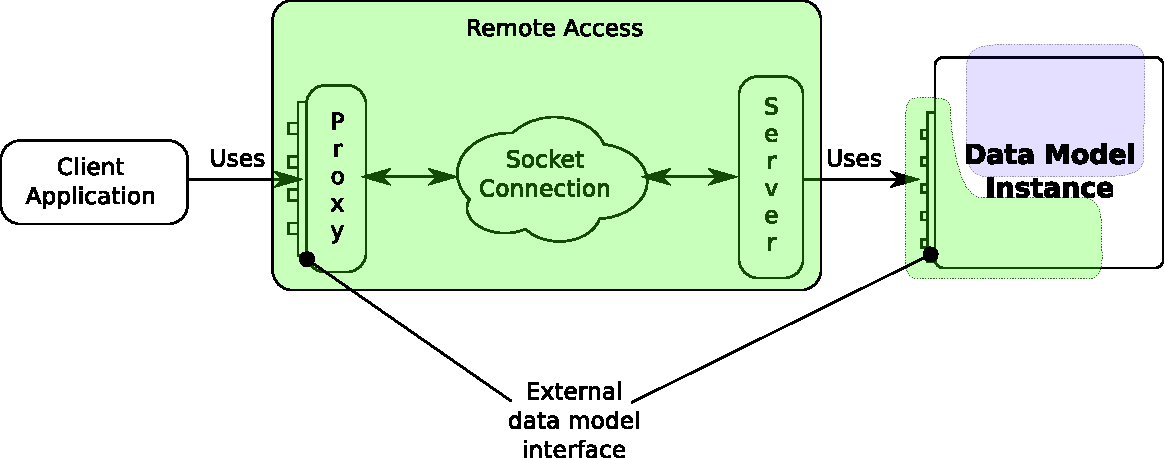
\includegraphics[scale=0.5]{img/remoteAccess.pdf}
\caption{A data model proxy interface and server is generated, to support transparent remote access to a data model instance. Coloured areas are auto generated code.}
\label{fig:remoteAccess}
\end{figure}


\subparagraph{Terminal test}

The generator also generates a program where a user can call the methods
of the external interface through a simple terminal.

\begin{figure}[h!]
\centering
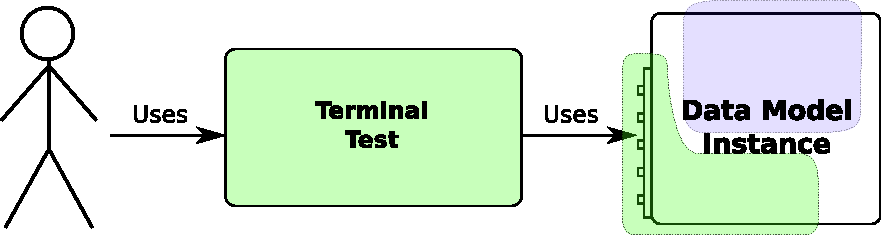
\includegraphics[scale=0.5]{img/terminalTest.pdf}
\caption{An terminal test program is generated to let a user test the methods in the external interface of a data model instance.}
\label{fig:terminalTest}
\end{figure}


\subparagraph{Web Interface}

It would also be possible to generate a web interface where a user
can interact with a data model instance through the external interface.
Javascript can be created to validate the value domains. We have created
an early prototype of this, but it requires a bit more work to be
perfected.

\begin{figure}[h!]
\centering
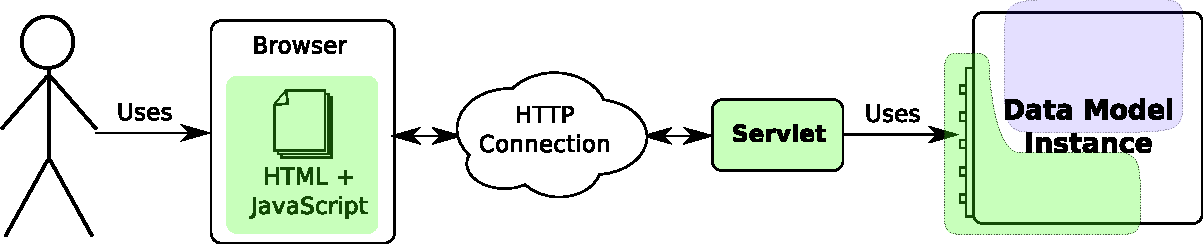
\includegraphics[scale=0.5]{img/web.pdf}
\caption{A web servlet for interacting with a data model instance together with HTML and Javascript for validating values on the client side, could be auto generated.}
\label{fig:web}
\end{figure}


\paragraph{Names and Packages}

It is important to us that the generated code can compile right away
without any changes, so we need to keep track of all imports and package
information. Since many of the generated interfaces and classes are
dependent on each other and on the runtime interface, any changes
to the naming conventions or the package structure would require lots
of changes to the generator code in many different places. To avoid
this we have abstracted out the naming conventions and the package
structure to a separate interface that takes care of all class names,
package names and package layout. This interface is then used all
over the generator. In this way it is easy to make changes to the
names of interfaces and classes or to the package structure of the
generated code. It is even possible to have several implementations
of the naming interface, so it is possible to switch between different
naming and package layout strategies.



\subsection{\label{sec:Runtime}Runtime System}

The runtime system is the module that is responsible for managing
all the data in a data model instance at runtime. This includes the
following tasks:
\begin{itemize}
\item \textbf{Data Containment: }Holding data that make up the current state
of a running data model instance, which includes all entities and
connections between entities.
\item \textbf{Index Containment:} Keeping and updating all indexes on the
data model instance.
\item \textbf{Transaction Execution:} Making sure that all transactions
are executed correctly.
\item \textbf{Data Persistence:} Taking care of the persistence of the data
model instance. 
\end{itemize}
The runtime implements a series of runtime interfaces, used by the
generated code. There could be many different implementations of the
runtime interface, each with different strategies and solutions on
how to solve these tasks. This way it is easy to switch between different
runtime implementations without any changes to the generated code,
or to the code written by the users.


\subsubsection{Runtime Interface}

In the creation of the runtime interface we have tried to make it
independent of how it would be implemented.

Since the runtime interface is non-generated code, it has no knowledge
of specific data models at compile time. It gets the information about
the specific data model that it should manage from the meta model
instance at runtime. Thus, in the runtime interface specific kinds,
relations and indexes are referred to by their index in the meta model
instance.

The runtime interface consists of a number of Java interfaces that
a runtime implementation must implement. These interfaces are:
\begin{itemize}
\item \texttt{IRuntimeFactory} - Given the meta model instance for a specific
data model it returns an \texttt{IDataModelInstanceFactory}
\item \texttt{IDataModelInstanceFactory} - Can load, create and delete individual
instances of a data model.
\item \texttt{IDataModelInstance} - Represents an instance of a data model.
Has methods to start and stop the instance and execute views and actions.
\item \texttt{IView} - Represents a view on the data model implemented by
the user.
\item \texttt{IAction} - Represents an action on the data model implemented
by the user.
\item \texttt{IResult} - Represents the result of executing a view or an
action on the data model instance.
\item \texttt{IDataModelView} - This is the interface that the user implementations
of actions are bound to through the auto-generated internal API interfaces
and classes.
\item \texttt{IDataModelUpdate} - This is the interface that the user implementations
of views are bound to through the auto-generated internal API interfaces
and classes.
\item \texttt{IIndex} - Represents an index on the data model.
\item \texttt{IEntity} - Represents an entity in the data model.
\end{itemize}
Any implementation of an EDMA runtime system must provide these interfaces
for the generated code to bind up against.


\subparagraph{Procedural vs Declarative Query Languages}

In EDMA queries to the data models are written in a procedural manner,
where the user describes an algorithm for how to construct the result,
using the structure of the data model to navigate and using set operations
to narrow or widen the result.

In SQL, queries are written in a declarative way, where the user describes
what the result should be, but not how to obtain it.

It is a subjective matter which of these approaches that feel most
natural, but if a user has an object oriented background, he is used
to get things done in a procedural manner.

One advantage of the declarative approach is that the underlying system
has freedom to analyze the query and try to find the most optimal
algorithm for creating the result.

But even though EDMA takes a procedural approach to obtain the result,
we can use abstraction to let the runtime system delay decisions and
do some amount of optimization on its own. One example of this is
the way sets and set operations are handled in the runtime system.


\subparagraph{Sets and set operations}

One of the important features the runtime system most provide is set
operations such as union, intersection and subtraction. But instead
of representing a set by a java class, we simply use an index that
the runtime system controls. In this way when the user asks the runtime
system to perform an intersection of two sets, all the runtime system
actually gets are the indexes of the sets to intersect and it returns
a new index that represents the intersection of the sets. But the
runtime does not actually have to perform the intersection at this
time. Only when the user actually wants to access or count the elements
in the set, the runtime must perform the intersection. In the case
of complicated queries that involves many set operations before the
final result is produced, the runtime system can analyze and optimize
how to perform these set operations. This method of postponing evaluation
until the result is actually used is known as lazy evaluation.

Especially in a runtime implementation that is backed by an SQL database,
the lazy evaluation is important to avoid sending lots of small queries
to the DBMS, but instead build a larger query behind the scene and
send it when the result is needed. This will both minimize communication
with the DBMS and give the DBMS better optimization opportunities.


\subparagraph{Value domains in the runtime}

Each value domain has its own handler in the meta model instances.
These value domain handlers take care of everything that has to do
with values. To the runtime system a value is simply a Java object
and every time the runtime system needs to do something with a value
(e.g. write it to a stream) it simply invokes the handler for that
specific value domain.


\subsubsection{Example Runtime System}

We have created an example runtime system that are written entirely
in Java. It stores the current state of the data model instances in
memory using standard Java collections like HashMap, HashSet, TreeMap,
TreeSet etc. This gives us a fairly fast implementation but with a
significant memory footprint.


\paragraph{Data Containment}

All the data of a running data model instance, is held in containers
called \emph{Kind Store, Relation Store} and \emph{Index Store}. They
contain all the data that is currently in the data model, as well
as uncommitted data.


\subparagraph{Kind Store}

Entities of any kind are stored in a Kind Store. There is one kind
store for each kind in the data model definition. A kind store is
backed by a hashmap, with a \texttt{Long} as key, and an \texttt{Entity}
object as value. The \texttt{Entity} object contains an object array,
holding the attribute values of the entity.


\subparagraph{Relation Store}

The relation store is used for storing connections between entities.
We have different Relation Store implementations based on cardinality
of the relation. Each end of the relation has a map that maps from
IDs to connected IDs. If the opposite end is a \emph{one} single IDs
are stored as values, if the opposite end is a \emph{many}, sets of
IDs are the values. Special implementations take care of removing
redundancy in self-relations by sorting the IDs before a connection
is inserted or retrieved. 


\paragraph{Index Containment}

As earlier mentioned, EDMA provides three types of indexes on kinds
and on relations: unique, compare and equals. In the example runtime
system the equals- and unique indexes are backed by hashmaps, and
the compare index is backed by a treemap using the NavigableMap interface.

Updates on the indexes are performed whenever a relevant entity is
created, deleted or relevant attributes are updated.


\paragraph{Transaction Execution}

The execution model is responsible for managing the execution of the
transactions. The execution model must ensure the ACID properties.

There are basically two ways of executing transactions. Either, transactions
can be executed sequentially, or they can be executed in parallel.
In most database systems, transaction execution is done in parallel,
using concurrency control mechanisms to secure data integrity. When
executing transactions in parallel, certain concurrency control mechanisms
are needed to ensure the isolation property. Concurrency control can
either be pessimistic or optimistic. 


\subparagraph{Pessimistic Concurrency Control}

In a pessimistic concurrency control mechanism, transactions acquire
locks on data, before they execute. In EDMA, the user writes the transactions
in pure Java, after the code has been generated. This means that EDMA
is not compiling or reading the user created transactions. This makes
it impossible for EDMA to know which parts of the data model the user
is accessing, and hence which parts should be locked.


\subparagraph{Optimistic Concurrency Control}

In the optimistic approach, all reads of a transaction are logged,
and the writes are done to a local cache only, until the commit phase.
In the commit phase it is checked that none of the reads has changed
before the writes are made permanent. If any of the reads has changed,
the entire transaction is canceled and re-executed at a later time.

It would be possible to implement a similar strategy in an EDMA runtime
system, but we have chosen not to do so in the example runtime system
because of: 1) The complexity of it, and the time it would take to
implement, 2) the bookkeeping overhead it would impose, and 3) it
would require that all transactions could risk to be canceled and
re-executed, which puts some heavy constraints on the side effects
that would be allowed inside a transaction. In Java it would be very
hard (if not impossible) to detect and warn about such unwanted side
effects and therefore this would break the illusion that a data model
instance is just a synchronized object.


\subparagraph{Sequential Execution}

The simplest way of obtaining 100\% ACID properties would be to execute
and persist all transactions completely sequentially. Although this
approach would probably be sufficient in many cases where performance
is not a big issue, we can easily get a better performance in a multi-threaded
environment by some parallelization of the process. There are two
ways we can parallelize the process without adding any significant
concurrency control overhead. The first one is to pipeline the process
into an execution step and a persistence step. The second way is to
parallelize views. 

In EDMA, we have chosen to make the actions run sequentially. However,
the sequential run has been pipelined into a two-step process: execution
and persistence. By having the process broken up in two independent
steps, one thread can run the execution of a transaction while another
thread runs the persistence of a previously executed transaction.


\subparagraph{Pipelining}

By pipelining the execution and the persistence, we do not have to
wait for a transaction to be persisted before we can start executing
the next one. Figure~\ref{fig:executionPipelineSimple} illustrates
the idea, representing the different transactions of threads by boxes
in different colors (each color belongs to one thread.)

\begin{figure}[h]
\centering
\subfloat[Simple execution pipeline, with an execution step and a persistence step. Each colored box represents a transaction. Each column represents a distinct time slice.] {\label{fig:executionPipelineSimple1}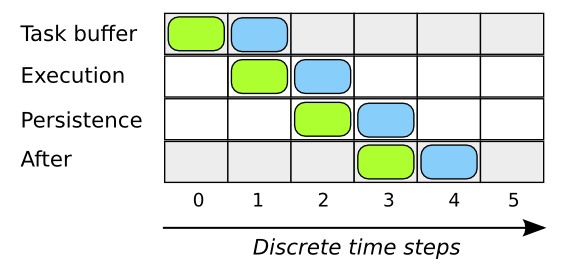
\includegraphics[width=0.5\textwidth]{img/executionPipelineSimple1.png}}\\
\subfloat[Here the persistence step blocks the execution step from fetching in new tasks to execute.]{\label{fig:executionPipelineSimple2}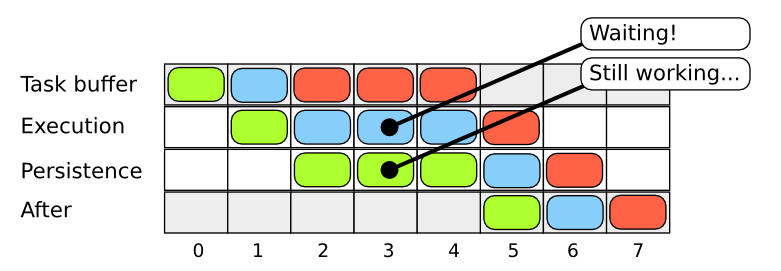
\includegraphics[width=0.7\textwidth]{img/executionPipelineSimple2.png}}
\caption{A simple pipeline helps parallellizing execution and persistance. However, blocking may occur.}
\label{fig:executionPipelineSimple}
\end{figure}In figure \ref{fig:executionPipelineSimple1} a thread starts a transaction,
represented by the green box, at time 0. At time 1, the execution
unit takes the green transaction from the task buffer, and executes
it, while another thread (blue) puts another transaction into the
task buffer. At time 2, the green transaction is handed over to the
persistence unit, while the blue transaction is going into the execution
unit. Now, we can have one thread doing the execution, while another
thread does the persistence. We still return control to the client,
only when the action called by the client has been persisted. Therefore,
the thread issuing the green transaction is blocked, until the green
transaction enters the After slot (only shown for pedagogical reasons).

Each of the two steps in the pipeline are sequentially executed, and
therefore the slowest of them decides the throughput of the complete
pipeline. However, if we add a buffer between the two steps, we can
smooth out the workload of each step, if some transactions are heavier
on the execution and others are heavier on the persistence. The goal
is to keep both the execution and the persistence mechanism as busy
(i.e. non-idling) as possible, with a minimum of waiting. This is
shown on figure~\ref{fig:executionPipelineBetter}. 

\begin{figure}
\centering
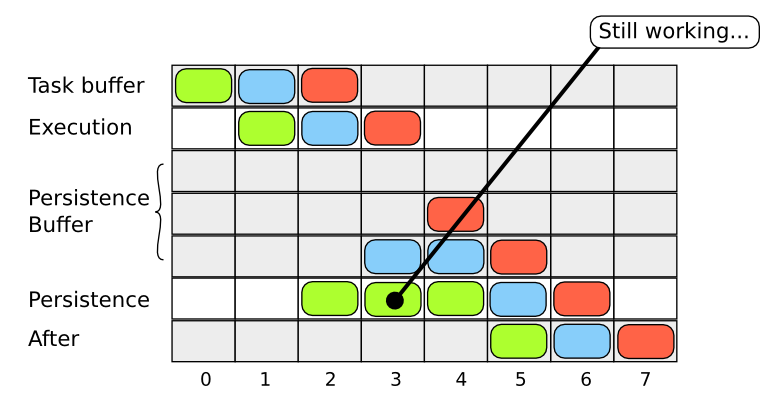
\includegraphics[width=0.7\textwidth]{img/executionPipelineBetter.png}
\caption{By adding a buffer between the execution step, and the persistence step, we can to some extend eliminate blocking of the pipeline.}
\label{fig:executionPipelineBetter}
\end{figure}


\subparagraph{Parallelization of Views}

The second parallelization method takes advantage of the distinction
we have made between the two types of transactions: \emph{actions}
and \emph{views. }Since we know that views can never change the state
of the data model it is safe to parallelize these. It is important
to notice here that even though views have nothing to persist, we
still need to send them through the entire pipeline and not let them
return control to the client thread before they have reached the persistence
step. The reason for this is the \emph{durability} property that we
wish to maintain. We do not want a view to reflect anything in the
data model that has not yet been persisted. If we let the views return
immediately after the execution step, we could get into a situation
where the view reflected the effect of an action that were still in
the persistence buffer, waiting to be persisted. If the persistence
of the action somehow failed, then the view would reflect a non-persisted
state of the data model. Therefore, execution of views is parallelized,
but views must sequentially pass through the persistence unit (which
then does nothing else than marking the view as persisted.)


\subparagraph{The execution algorithm used in the example runtime system}

In EDMA the executor and the persistence module are run in two separate
threads. \emph{Actions} are executed sequentially in the executor
thread while \emph{views }are executed in parallel in their client
threads. The executor has two modes: action-mode and view-mode. When
in action-mode it executes actions in sequence. When in view mode
it lets views execute in their client thread in parallel. When it
switches from view-mode to action-mode, it waits for all current running
views to finish their execution before it starts executing actions.

The pseudo code for the main loop of the executor can be seen in algorithm~\ref{alg:Execution-main-loop}.

\begin{algorithm}[H]
\begin{lstlisting}[tabsize=4]
loop
	t <- get next task from queue
	if(t is an action)
		if(not in action-mode)
			wait for running views to finish
			set mode to action-mode
		executeAction(t)
	else
		set mode to view-mode
		allow t to execute in client thread
\end{lstlisting}


\caption{\label{alg:Execution-main-loop}Execution main loop}
\end{algorithm}


In the current implementation of the executor, a single FIFO queue
is used for both \emph{actions} and \emph{views}. This provides good
fairness, but if \emph{actions} and \emph{views} are highly interleaved,
in the sense that there are no large groups of \emph{views} that are
not interrupted by \emph{actions}, then we do not get much parallelization.
We could instead have two FIFO queues, one for \emph{actions} and
one for \emph{views.} In that way, it would be possible to parallelize
the views in larger chunks. We could then have an algorithm that would
process \emph{views} until the \emph{view} queue is empty and then
switch to process \emph{actions} until the \emph{action} queue is
empty. In order to avoid starvation we could set a maximum number
of transactions to process before looking to the other kind. It is
important to notice here that although this strategy could lead to
a non-chronological execution of transactions, the chronology would
be preserved within each client thread. This is guaranteed, since
whenever a client is executing a transaction, control is never returned
to the client thread before the transaction has been both executed
and persisted.


\paragraph{\label{sub:Persistence}Data Persistence}

In EDMA the current state of the data model is kept in RAM, which
is a volatile storage that is lost in the case of a power failure,
or any other type of system failures. For many applications it is
crucial to store data in a more persistent way so the state of the
data model can be preserved and regenerated even in the case of a
power failure, system reboots an so on. Sometimes it is enough to
store data on a local hard drive, other times applications need a
more secure persistence where data is stored in several different
places.

In EDMA the persistence module is operated on through a simple interface,
making it possible to have different persistence module implementations,
with different strategies for data persistence. Although there is
currently only one implementation, switching between different persistence
strategies can be made into a matter of changing one line of code
for the user. In the following, we describe the strategy that we have
implemented in this project.

Every time an action is executed in EDMA, it generates a sequence
of primitive operations. If the execution fails for some reason, these
operations are rolled back (as described in section \ref{sub:Transactions})
and nothing is sent on to the persistence module. If the action executes
successfully, the sequence of operations that describe all changes
made to the state of the data model instance, is put into an object
called a \emph{persistence unit}. Besides the sequence of operations,
the persistence unit also has two callback functions, one to call
if the data is successfully persisted and another one to call if the
persistence of the data fails for some reason. This persistence unit
is then handed over to the persistence module and whenever the persistence
module has persisted the data or failed in its attempt to do so, it
will call the corresponding callback function on the persistence unit.

This effectively means that every time an action successfully makes
changes to the state of the data model instance, these changes are
persisted as an atomic unit. So when the need for recovery arises,
these changes can be replayed in sequence to re-generate the state.
This also means that a full history of states of the data model is
preserved and could be re-generated if needed.

It is important to note here, that to honor the durability property,
a persistence unit may never be considered successfully persisted
before all preceding persistence units has also been successfully
persisted. Actually \emph{views} also need to pass through the persistence
module as persistence units although they do not have anything to
persist. The reason for this is that the result of a view is not considered
valid or durable before all preceding actions have been successfully
persisted. If the persistence module fails to persist a persistence
unit, then all succeeding persistence units must also be considered
failed, as shown in Figure~\ref{fig:executionPipelineFailing}.

\begin{figure}[h]
	\centering
	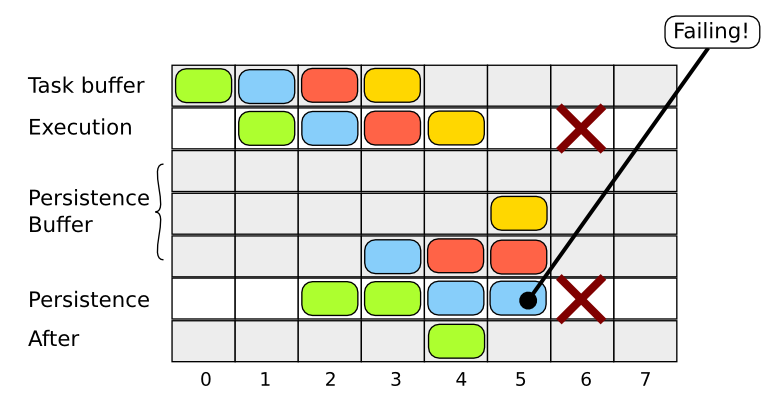
\includegraphics[width=0.7\textwidth]{img/executionPipelineFailing.png}
	\caption{If the persistence module fails, it stops, together with the execution module, and both the task buffer and the persistence buffer is emptied.}
	\label{fig:executionPipelineFailing}
\end{figure}

This may seem like a very bold form of error handling -- shutting
down the whole system, when one thread's transaction fails to be persisted.
However, if the persistence module fails, it means that the disk failed
to write data to the log file, which indicates that there might be
a problem with the disk. Therefore, it wouldn't make sense to continue
writing any subsequent transaction to that file. The failure could
be caused by bad sectors on the disk, which means that it could be
possible to successfully write to a new log file. A clever implementation
of the persistence module (in contrast to our simple proof-of-concept
implementation) could retry writing to the file a number of times,
and upon failure, start writing to a new log file. If that also fails,
writing to another disk could be attempted. Taking it even further,
if writing to any of the disks fails, the system could fall back on
writing to a network socket.

If the system really fails to persist a transaction, EDMA is closed
down, and an administrator will have to manually start the system
again (after running any disk-utility to flag out bad sectors.) Upon
restart, the system reads the whole log file, restoring the data model
to a state identical to the one at the time before the crash.


\subsubsection{SQL Runtime System}

When we planned this thesis, we intended to include a SQL implementation
of the runtime system that would store the data model instances in
a traditional SQL database. 

There are several reasons why this would be a good idea. First, databases
are very mature as a technology, and the database engines are highly
sophisticated and optimized for giving high throughput, serving many
concurrent users, and storing large amounts of data. It would add
some extra work for the user in setting up and connect to a data base,
but this would be rewarded by good scalability in the amount of data
that could be stored. He could always create prototypes with the embedded
java runtime and then switch to the SQL runtime when the need for
storing more data showed up.

However, we chose not to implement an SQL database backed runtime,
because it showed to be more complicated than expected, after we had
invented our value domains system. In an SQL database, there is a
finite set of primitive value domains. In our value domain system,
value domains can be constructed arbitrarily complex, and therefore
there exists an unbounded number of different value domains. This
makes it a non-trivial task to map our entities to SQL tables. It
came to a point where we either had to give up the value domain system
or the SQL implementation due to time constraints.

Given our focus in this project, of investigating the possibilities
of reducing the efforts of coming from a conceptual model to a working
prototype and explore alternative ways of working with data models,
we chose to keep the value domain system and postpone the SQL implementation.


\subsubsection{JDBM3 Runtime System}

The example runtime has the limitation that it can only hold as much
data, as the RAM can contain. Further more, there is a significant
memory footprint in using the example runtime, since all data values
are being wrapped in a number of Java objects, taking up memory (see
the Evaluation section for more details.) For that reason, we have
chosen to exploit the flexibility of the EDMA system, and implemented
the usage of disk-backed sets and maps, using the open source framework
JDBM3. JDBM3 is a key-value store with a number of disk-backed collections,
with the goal of being able to handle billions of items without being
limited by memory. The point of using JDBM3 in EDMA was to have both
large amounts of data, but also to make it possible to perform set
operations on large sets (for results or partial results in actions
and views.)

It turned out that there were some hindrances, making it difficult
to obtain good performance using JDBM3. In order to reach a good performance
level, we need to disable auto-commit in JDBM3. However, having to
manually call commit would require substantial changes in the infrastructure
of the runtime system, therefore complicating the task more than the
benefit added. Further more, it was found that JDBM3 has a bug, preventing
EDMA from using multiple threads access the data store. That said,
since the authors of JDBM3 keep the project alive with frequent updates,
it would be a matter of time before the bug gets fixed.




\section{\label{sec:Evaluation}Evaluation}

In this section, we address the issue of evaluating the EDMA system,
both with respect to its functional usability, and with respect to
a few performance parameters. Since one of the main points with EDMA
is to make it easy for the user to come from an idea of a data model,
to working implemented code reflecting that model, we briefly discuss
the steps that are required for doing so.

Although performance hasn't been the main focus of this project, we
have created a few simple performance tests. These are presented and
briefly discussed in Appendix \ref{sec:PerformanceEvaluation}.


\paragraph{Functional Evaluation}

Evaluating the usability of EDMA can be done by asking a series of
questions:
\begin{itemize}
\item How easy or difficult is it to create a new data model?
\item How easy or difficult is it to change an existing data model?
\item How easy or difficult is it to implement actions and views?
\end{itemize}
One way of measuring the complexity of using EDMA would be to get
a group of people to read the tutorial, and then carry out a list
of predefined tasks. The time it would take to complete each task
would then depict the complexity of the various parts of the system.
Another way of measuring the complexity, is to count the number of
steps it takes to optimally solve a certain task.

In answering these questions, we need a standard measure, to describe
how the tasks are carried out. As a measure, we count the number of
steps involved, and comment on the complexity of the steps.

The flow of creating a data model implementation can be divided into
4 phases:
\begin{itemize}
\item 1 -- Model definition
\item 2 -- Code generation (run the EDMA compiler)
\item 3 -- action and view implementation (create the necessary code in
the action and view stub classes)
\item 4 -- data model instantiation (create an instance of the data model
to use in the external application)
\end{itemize}
We see designing and implementing a concrete data model as an iterative
process, where the user switches between phase 1, 2 and 3 in a number
of iterations. In a prototyping scenario, where not all business requirements
may be strictly given, new requirements or ideas may influence and
change the design for a number of iterations. The user might work
in a typical prototyping scenario, going in and out of different work
phases in an undetermined order:
\begin{itemize}
\item Recognition and definition of the domain specific value domains
\item Recognition of the need for modeling a certain kind, relation, singleton,
action or view
\item Creation or refining of the data and interface definition files
\item Generation of code and implementation of actions and views
\end{itemize}
In many prototyping scenarios, the user will not be able to create
the full data model in one iteration. Therefore, it is important that
the user can easily go back and update the definition files, re-generate
the code, and fill out stub code of newly created actions and views.
And if the latest change to a definition file has resulted in broken
code, it must be easy to find and correct the files in question. In
the following, we discuss the four steps that make up the process
of using EDMA.


\paragraph{Data Definition}

Data definition is done by creating one, or many, data definition
files, adhering to the syntax of the EDMA definition language. The
definition of the kinds will itself result in a number of iterations,
where the user realizes the need for value domains, relations and
actions and views. For example, when creating the Person, the user
realizes the need for the attribute value domains Name, Date, PhoneNumber
and Balance. The following is noticed.
\begin{itemize}
\item Each value domain and each relation takes up one line of code. Each
kind takes up one line for the declaration, plus one line for each
attribute. Actions and views take up one line for the declaration,
one line for the description, one for the error code, and one line
for each input and output.
\item The number of relations will roughly be following the number of relations.
\item The number of actions will often be around twice the number of kinds
and relations (the user can have creation and deletion actions for
each kind and for each relation, and additional views and actions.)
\item Creating the value domains may be time consuming the first time it
is done, but as the user creates subsequent data models, he will find
out that there is a common set of value domains that are needed in
many data models. Therefore, the user might create a file for holding
the basic value domains needed (Year, Month, Day, Date, Hour, Minute,
Second, Time, PosInt, NegInt, etc.)
\end{itemize}
Because of the number, and line-span, of actions and views, we estimate
that writing the action and views is the most time consuming process,
when writing the edma-files.


\paragraph{Running the EDMA Compiler}

Running the EDMA compiler is a question of running a Java program.
If there are errors in any of the edma-files, the compiler gives the
user a message stating the error type, and the location of the error.
After the compiler has been run, the user should make sure that the
IDE shows the newest version of the directory listing (in Eclipse,
this is done by right clicking on the project folder, and choosing
Refresh.)


\paragraph{Implementing Actions and Views}

The stub code that is generated for actions and views purposefully
contains a syntax error. In that way, the user can quickly find the
action and view stub classes that need to be filled out

If the user has already implemented some actions and views, and later
decide to recompile the edma-files, the existing actions and views
will be kept.


\paragraph{Instantiation}

Instantiating the created data model is done in very few steps, by
calling a static method to retrieve a meta model instance, and creating
a runtime factory by which to obtain a model instance.


\subsubsection{Evaluation of Tutorial}

One way of assessing the usability of the EDMA system, is to let a
user complete the tutorial (Appendix \ref{sec:EDMAtutorial}), and
note down the time it takes to complete the individual steps. 



\section{Conclusions\label{sec:Conclusions}}

The main focus in the thesis have been to investigate a model driven
approach to handling data manipulation and persistence in an object
oriented language. The goal has been to eliminate a series of issues
that often arise in projects involving object oriented languages,
when coupled with external database systems.

Using EDMA, a user is able to transform a conceptual model into usable
code, shortening the path between getting an idea for a data model,
and having a running implementation. This is done through three steps: 
\begin{itemize}
\item First the user must define a conceptual data model, and write it in
the created EDMA data definition language. 
\item Then he must define the transaction signatures on the data model. 
\item At last, the user must implement the transactions in Java.
\end{itemize}
A Java interface containing the defined transactions is created, and
can be used from any java application. The EDMA runtime system is
designed in a modular way, allowing for future optimization of the
persistence mechanism, the set manipulations and the runtime data
containment.
\begin{itemize}
\item transaction language would be interesting\end{itemize}




\section{Future Work}

There are a number of features that could still be implemented in
EDMA, especially related to usability. By trying to use EDMA in various
situations, we have found that the time the user spends on reaching
a readily usable data model can be reduced. For example, we could
auto-generate CRUD actions and views (methods for Creating, Reading,
Updating and Deleting).
\begin{description}
\item [{CRUD~Actions~and~Views}] One way of helping the user, is to
auto-generate actions and methods for creating, reading, updating
and deleting (CRUD) data entities. At first, it was our philosophy
that the user should only have the actions and views defined by himself,
in order to not clutter the API with functions that wouldn't be used.
However, by creating data models with our system ourselves, we have
found that we almost always end up creating the most basic actions
and views for each kind:\end{description}
\begin{itemize}
\item Insert a new entity of a given kind.
\item Get entities based on attribute values (defined from indexes).
\item Update one of the mutable attributes in a kind.
\item Delete an entity.
\end{itemize}
As of the current version of EDMA, the user has to define these 4
methods in an \texttt{.edma}-file, and implement them in the generated
Java stub-code. Further more, for each relation, the user often needs
to connect two or more entities, or to delete a connection between
two or more entities.

It would require two changes to the system, to auto-generate CRUD
and relation-methods:
\begin{itemize}
\item Changing the compiler to add meta-actions and meta-views, for each
kind and each relation.
\item Changing the generator to generate the implementations of the actions
and views, instead of having the user to fill in stub-code in the
auto-generated actions and views.
\end{itemize}
Both of these two tasks are trivial, and could be implemented in a
short time. It would spare the user for the tasks of implementing
tedious, simple actions and views, at the cost of putting possibly
unused functions in the generated data model API.
\begin{description}
\item [{Multiple~APIs}] In a setting with many users, it is often possible
to distinguish between access rights of users. An extension to the
data model would be to group actions and views into interfaces. For
example, an interface for an Admin user could contain one set of actions
and views, while an interface for a User could contain a different
set of actions and views.
\item [{Simplifying~the~Value~Domain~System}] The value domain system
can be made more simple, by removing some of the primitive types.
For example, the types Integer and Long could be substituted with
a single Number type, and the Float and Double types could be substituted
with a single Decimal type. By inspecting range constraints it is
possible to determine best the representation on the underlying system
(in our case Java.)\end{description}



\appendix

\section{\label{sec:EDMAtutorial}EDMA tutorial}

This tutorial will be loosely based on the Diving School example in
the report. If you have not already read through this example, now
would be a good time to at least skim through it.

To follow this tutorial you need eclipse (or another Java Development
Environment) and the EDMA.jar file. In this tutorial we will take
you through all the steps that are required to build a working example
of the Diving School Course Registration System with EDMA. This includes
the following steps:
\begin{itemize}
\item Set up a new EDMA project in eclipse.
\item Define global value domains.
\item Define the data model for the course registration system.
\item Define the actions and views for the course registration system.
\item Implement the actions and views.
\item Connect to the runtime and use the course registration system.
\end{itemize}

\subsection{Set up a new EDMA project}
\begin{enumerate}
\item Create a new java project in eclipse named \emph{DivingSchool}.
\item Right click the project in package explorer and choose \emph{new}
\(\rightarrow\) \emph{Folder}. Write \emph{lib} as the name of the
folder and click \emph{finish}.
\item Copy EDMA.jar to the newly created folder. Right click the project
in package explorer and choose \emph{refresh}.
\item Right click the project in the package explorer and choose \emph{properties}.
Now click on \emph{Java Build Path} in the left part of the window.
In the right part of the window click on the tab \emph{Libraries}
and then on the button \emph{Add JARs... }Navigate to the \emph{lib}
folder and choose the EDMA.jar file. Click \emph{OK} in both windows.
\item Right click on the project in package explorer and choose \emph{new}
\(\rightarrow\) \emph{Folder}. Write \emph{edma} as the name of the
folder and click \emph{finish}. Right click on the newly created edma
folder and choose \emph{new} \(\rightarrow\) \emph{File}. Write Common.edma
as the file name and click \emph{finish}. Right click the new Common.edma
file and choose \emph{Open with} \(\rightarrow\) \emph{Text Editor.
}Now write this line exactly:
\begin{lstlisting}[basicstyle={\scriptsize}]
ValueDomain Name : String[1..MAX]
\end{lstlisting}
Make sure you write exactly the above line and then press \emph{Ctrl-S}
to save the file. You have now created your first global value domain
called Name. The values in Name are strings that are at least 1 character
long. You will learn more about how to create value domains in a moment.
\item Right click on the project in package explorer and choose \emph{new}
\(\rightarrow\) \emph{Class}. Write Make as the name of the class
and click finish. Write this code into the class:
\begin{lstlisting}[basicstyle={\scriptsize},breaklines=true,language=Java,tabsize=2]
import edma.generator.EdmaGenerator;

public class Make
{
	public static void main(String[] args)
	{
		//This will be the name of the environment
		String environmentName = "DivingSchool";
		//This is the path to the folder with your EDMA files
		String edmaSrcDir = "C:/Workspace/DivingSchool/edma";
		//This is the path to the java src folder
		String javaSrcDir = "C:/Workspace/DivingSchool/src";
		//This is the root package of the generated code
		String rootPackage = "tutorial";
		new EdmaGenerator(environmentName,
						  edmaSrcDir,
						  javaSrcDir,
						  rootPackage).make();
	}
}
\end{lstlisting}
Make sure you replace the paths with the actual paths on your machine.
Now right click on this class in the package explorer and choose \emph{Run
As} \(\rightarrow\) \emph{Java Application}. The output should look
like this: 
\begin{lstlisting}[basicstyle={\scriptsize}]
Gathering and compiling input files...
Generating environment generator...
Generating value domain classes...
Deleting generated directories...
Writing generated java files...
All done!
\end{lstlisting}
Now right click the project in package explorer and choose \emph{refresh}.
You should now see some generated packages in the project. Every time
you make any changes to your EDMA files you must run this Make class
and refresh the project.
\end{enumerate}
When you run the Make class it creates a new instance of the EdmaGenerator
class and calls the make() method on it. The compiler now looks for
files in the edma folder and its sub folders that has the extension
``.edma''. All these files are then compiled to a meta model and
the generator then uses this meta model to generate all the java interfaces
and classes. If you look at the generated packages and java files,
you should see a package called \emph{generated} as a sub package
of\emph{ tutorial.divingschool }(depending on the names you gave for
the project and root package)\emph{.} This package and everything
inside it will be deleted and re-generated whenever you call the make()
method on the generator class, so you should never put anything into
this package or make changes to the files inside this package or any
of its sub packages.


\subsection{Define Global Value Domains}

Now you should have a newly created EDMA project up and running with
one global value domain called Name. Now lets define some more global
value domains. We need a Date value domain that contains a year, a
month and a day of month. All values from this value domain should
be valid dates. First lets create the value domains Year, Month and
DayOfMonth:
\begin{lstlisting}[basicstyle={\scriptsize}]
// Year, Month and DayOfMonth
ValueDomain Year : Integer[0..9999]
ValueDomain Month : Integer[1..12]
ValueDomain DayOfMonth : Integer[1..31]
\end{lstlisting}


Add those value domains to the Common.edma file. You can make comments
in edma files just like in java files with // and /{*} ... {*}/.

Before we continue, we will take a quick look at how these value domains
work. Run Make and refresh the project. Now create a new Test class
in the default package that looks like this:

\begin{lstlisting}[basicstyle={\scriptsize},breaklines=true,language=Java,tabsize=2]
import tutorial.divingschool.generated.valuedomains.Year;
import edma.valuedomains.exceptions.InvalidValueException;

public class Test
{
	public static void main(String[] args)
	{
		//A valid year
		Year foo = Year.create(1988);
		System.out.println(foo.toString());
		foo = Year.fromString("1807");
		Year bar = Year.create(1807);
		System.out.println("foo equals bar: " + foo.equals(bar));
		System.out.println("Is -11 a valid year: "
			+ Year.isValidYear(-11));
		System.out.println("Is 1990 a valid year: "
			+ Year.isValidYear(1990));
		//Lets try to make an invalid year:
		try
		{
			bar = Year.create(-54);
		}
		catch(InvalidValueException e)
		{
			System.out.println(e.getMessage());
		}
	}
}
\end{lstlisting}


As you can see from this code there are a few static methods on the
Year class that can be used to create new values from the Year value
domain. You can also take a look at the generated Year.java file to
see all the methods. 

Now we can create the Date value domain as a \emph{Struct} value domain
that uses the Year, Month and DayOfMonth value domains. Add the following
to the Common.edma file:
\begin{lstlisting}[basicstyle={\scriptsize}]
//Date
ValueDomain Date : Struct
{
	year : Year,
	month : Month,
	day : DayOfMonth
}
\end{lstlisting}


Notice that in a \emph{Struct} value domain you can only refer to
value domains that are defined elsewhere. The order is not important,
you can define Year, Month and DayOfMonth before or after Date or
even in a separate file if you want. But you can not use the basic
value domains like String, Integer etc in a \emph{Struct} value domain.
So this is NOT possible:

\begin{lstlisting}[basicstyle={\scriptsize}]
//Invalid definition of Date
//Will NOT compile
ValueDomain Date : Struct
{
	year : Integer[0..9999],
	month : Integer[1..12],
	day : Integer[1..31]
}
\end{lstlisting}


Now run Make and refresh the project. The Date value domain is a \emph{Struct}
value domain that are build from other value domains. Each \emph{field}
in a \emph{Struct} value domain consist of a name and a value domain.
A \emph{field} in a struct can be optional, which means that the value
may be \emph{null}. To make a field optional all you have to do is
add a question mark after the name of the field. Here is an example
of a Struct value domain with some optional fields:

\begin{lstlisting}[basicstyle={\scriptsize}]
//Value Domain with optional fields
ValueDomain FooBar : Struct
{
	foo? : SomeValueDomainName,
	bar : SomeValueDomainName,
	foobar? : AnotherValueDomainName
}
\end{lstlisting}


Here foo and foobar are optional so they may be \emph{null}. If a
field is not optional then a NullPointerException is thrown if it
is set to \emph{null}.

\emph{Struct} value domains has a natural order where the significance
of the fields follows their position in the \emph{Struct}, with the
first field being the most significant and the last field least significant.
So if we had put the fields in another order, then dates would not
sort properly when using their natural order. Here is some examples
of how you can create values in the Date value domain.
\begin{lstlisting}[basicstyle={\scriptsize},breaklines=true,language=Java,tabsize=2]
import tutorial.divingschool.generated.valuedomains.Date;

public class DateTest
{
	public static void main(String[] args)
	{
		//Create a date with the create() method
		Date foo = Date.create().year(2012).month(2).day(15);
		System.out.println(foo.toString());
		//Create a date from a string representation of the date
		Date bar = Date.fromString("(2012, 3, 4)");
		
		//What happens if we create an invalid date like this 2012-2-30
		Date notValid = Date.create().year(2012).month(2).day(30);
		System.out.println(notValid.toString());
	}
}
\end{lstlisting}


Notice how the creation uses fluid interfaces to make it easier too
read the code. This can be very useful if you create struct value
domains with many fields. There is a separate interface for each field
you set that returns the interface to set the next field, so it is
not possible to leave out a field without getting a compile error
from the java compiler. Try it out, write Date foo = Date.create().year(1988).day(15)
and see that the compiler will not accept it because the month is
missing. Also the order of the fields is fixed when creating the values,
so Date.create().month(5).year(1788).day(7) will not compile either.

At first this strictness in the creation can seem a little rigid,
but if you later on add another field to a struct value domain, then
the compiler makes sure that you take this new field into account
everywhere you create values with that value domain.

If you want, try to create a TreeSet<Date> and put some dates into
it, they should be correctly sorted by their natural order when you
iterate over the set.

When creating a Date value, it is automatically tested that the year,
month and day are within the allowed limits for their value domains,
but what about invalid dates as 30/2/2012? These are not caught at
the moment. We can add a user implemented constraint to do this:

\begin{lstlisting}[basicstyle={\scriptsize}]
//Date
ValueDomain Date : Struct
{
	year : Year,
	month : Month,
	day : DayOfMonth
} Constraints[validDate]
\end{lstlisting}


This is done by adding the keyword \emph{Constraints }followed by
a comma separated list of names in square brackets. In this case we
only added one constraint. Now run Make and refresh the project. Try
to run the DateTest class above again and see what happens. It should
throw an exception saying that the validDate constraint is not implemented
and where you can implement it. Navigate to the class mentioned in
the exception. It should look like this:

\begin{lstlisting}[basicstyle={\scriptsize},breaklines=true,language=Java,tabsize=2]
package tutorial.divingschool.usercode.valueconstraints.date;

import tutorial.divingschool.generated.valuedomains.Date;

/**
 * This class is the implementation class for the Date constraint validDate
 * No description given
 */
public class ValidDate
{
    /**
     * Checks the validDate constraint for the Date value domain.
     * No description given
     * @param date  The instance value to be checked
     * @return      the reason the constraint is violated, or <tt>null</tt> if
     *              the constraint is not violated
     */
    public static String checkValidDate(Date date)
    {
        // Implementation of constraint validDate
        // WARNING : Any code outside the following begin and end tags
        // will be lost when re-generation occurs.
        
        // EDMA_non-generated_code_begin
        
        //TODO: Implement the constraint validDate here...
        return "Constraint not implemented. Implement in tutorial.divingschool.usercode.valueconstraints.date.ValidDate";
        
        // EDMA_non-generated_code_end
    }
}
\end{lstlisting}


The class is in a sub package of the \emph{usercode} package. All
classes that you need to put code into will be placed in the usercode
package or its sub packages. Now lets implement the validDate constraint
to only allow valid dates. This involves checking for leap years.
Be sure to only put your code between the \emph{EDMA\_non-generated\_code\_begin}
and the \emph{EDMA\_non-generated\_code\_end} tags, since anything
outside these tags will be re-generated when you run Make (except
any imports you might add, these will be preserved too). Now try to
add the following code between the \emph{EDMA\_non-generated\_code\_begin}
and the \emph{EDMA\_non-generated\_code\_end} tags: 

\begin{lstlisting}[basicstyle={\scriptsize},language=Java,tabsize=2]
    // EDMA_non-generated_code_begin
    int day = date.day().value();
    if(day <= 28) return null;
    switch(date.month().value())
    {
      case 2:
        if(day > 29) return "February can not have more than 29 days";
        // day == 29
        int year = date.year().value();
        if(year % 4 == 0 && (!(year % 100 == 0) || year % 400 == 0)) return null;
        return Integer.toString(year)
          + " is not a leap year, so February can not have 29 days";
      case 4:
      case 6:
      case 9:
      case 11:
        if(day <= 30) return null;
        return "April, June, September and November can not have more than 30 days";
      default:
        return null;
    }
    // EDMA_non-generated_code_end
\end{lstlisting}


As you see here the return value is a \emph{String}. You should return
\emph{null}, if the value is valid, otherwise you should return an
error message that says why the value is not valid. After you have
updated this file, try to run the DateTest again. This time only the
invalid dates like 30/2/2012 should fail.

With user implemented constraints you can make value domains that
are very precise in which values they accept and which they do not
accept. You should always try to make your value domains as precise
as possible, because then you will catch malformed input as early
as possible. The value domains are your guarantee that the input to
and output from your \emph{actions} and \emph{views} are valid. As
an example of a very specialized value domain, we will make a value
domain called FunnyInt that only contains positive integers that are
even, but not dividable by 10:

\begin{lstlisting}[basicstyle={\scriptsize}]
//FunnyInt
ValueDomain FunnyInt : Integer[1..MAX] Constraints[even, notDividableBy10]
\end{lstlisting}


Add the above to your Common.edma file and then run Make and refresh
the project. Now find the file \$\{project\}.usercode.valueconstraints.funnyint.Even.java
and replace the code between the \emph{EDMA\_non-generated\_code\_begin}
and the \emph{EDMA\_non-generated\_code\_end} tags with this:

\begin{lstlisting}[basicstyle={\scriptsize},language=Java,tabsize=2]
if(funnyInt.value() % 2 == 0) return null;
return funnyInt.value() + " is not even!";
\end{lstlisting}


In the same sub package find the file NotDividableBy10.java and replace
the code between the \emph{EDMA\_non-generated\_code\_begin} and the
\emph{EDMA\_non-generated\_code\_end} tags with this:

\begin{lstlisting}[basicstyle={\scriptsize},language=Java,tabsize=2]
if(funnyInt.value() % 10 == 0) return funnyInt.value() + " is dividable by 10!";
return null;
\end{lstlisting}


Make a test class and try out your new FunnyInt value domain.

We actually do not need the FunnyInt value domain in the course registration
system after all, so feel free to delete it from the Common.edma file
and regenerate. When you do this, you will notice that the Even.java
and NotDividableBy10.java files are still there, but now they do not
compile because the FunnyInt value domain no longer exists. You will
have to delete these files yourself. EDMA will never delete files
inside the usercode package or its sub packages. Only stuff outside
the \emph{EDMA\_non-generated\_code\_begin} and the \emph{EDMA\_non-generated\_code\_end}
tags will be overwritten by EDMA in the \emph{usercode} package and
its sub packages. But keep in mind that files you put in the \emph{generated}
package or its sub packages will be deleted by EDMA.

Now lets make the value domains that we need to create the Person
Kind. The Person Kind should have a name, an email, a mobile phone
number and a credit balance. The credit balance should be a non-negative
integer, since we do not allow negative credit. We already have a
Name value domain that is just a String of length 1 or more. Lets
make the other value domains:

\begin{lstlisting}[basicstyle={\scriptsize}]
//Email
ValueDomain Email : String[3..MAX]
//Mobile
ValueDomain Mobile : String[8]
//Credit
ValueDomain Credit : Integer[0..MAX]
\end{lstlisting}


As seen here the String value domains can both have a length range
like 3..MAX and 3..256 or it can just have a single length value like
in the mobile value domain. This means that a value from the mobile
value domain must be a string that are exactly 8 characters long.
We could also have used the notation 8..8 which is the same.

String value domains can also have regular expressions added to them.
These are added in square brackets after the length constraints. The
syntax for the regular expressions should be just like you would write
it in java as a hard coded string surrounded by double quotes. Lets
add a regular expression to the Email value domain and the Mobile
value domain:

\begin{lstlisting}[basicstyle={\scriptsize}]
//Email
ValueDomain Email : String[3..MAX]
["[\\w-]+(\\.[\\w-]+)*@[A-Za-z0-9]+(\\.[A-Za-z0-9]+)*(\\.[A-Za-z]{2,})"]
//Mobile
ValueDomain Mobile : String[8]["[0-9]+"]
\end{lstlisting}


This is not a perfect email regular expression, but it serves fine
as an example of how to use regular expressions on String value domains.
In the mobile regular expression we do not need to test that the length
is 8, since this is already being tested in the length constraint.
You should try it out now by making some valid and invalid emails
and mobile phone numbers in a test class.

The last thing we will look at before we move on to the data model
is how to create a \emph{List} value domain. As an example we will
create a value domain where the values are lists of dates:

\begin{lstlisting}[basicstyle={\scriptsize}]
//DateList
ValueDomain DateList : List<Date>
\end{lstlisting}


Run Make and refresh the project. Now here is some examples of how
you can create and use values from the DateList value domain:

\begin{lstlisting}[basicstyle={\scriptsize},language=Java,tabsize=2]
DateList myDateList = DateList.begin()
								.add(Date.fromString("(2012, 2, 1)"))
								.add(Date.fromString("(2012, 4, 5)"))
								.add(Date.fromString("(2012, 6, 26)"))
								.end();
System.out.println(myDateList);		
for(Date date : myDateList)
{
	System.out.println(date);
}

DateListBuilder builder = DateList.begin();
for(int i = 1; i <= 29; ++i)
{
	Date d = Date.create().year(2012).month(2).day(i);
	builder.add(d);
}
DateList datesInFebruary = builder.end();

System.out.println("The dates in february 2012:");
for(Date date : datesInFebruary)
{
	System.out.println(date);
}

DateList someDates = DateList.fromString("((1999,1,3),(1988,2,5),(1745,3,4))");
System.out.println(someDates);
DateList empty = DateList.fromString("()");
System.out.println(empty);
\end{lstlisting}


It is important to notice that like all other values from value domains,
list values are also immutable. The value is not created until the
end() method is called on the builder interface and when the value
is created, it can never be changed. So in the shown example the DateList
datesInFebruary will always contain the same dates in the same order
that they where added to the builder.

\emph{List} value domains has a natural order, where the elements
are compared one by one from the beginning of the lists. So if we
have lists of integers, then (1,3) is greater than (1,2,3), but (1,2)
is smaller than (1,2,3). This is the same way that Strings in java
is naturally ordered as lists of characters. 

This is all you need to know about value domains for now. 


\subsection{Defining the Data Model}

Create a new file in the edma folder called CourseRegistration.edma.
This file will contain our definition of the course registration data
model. Write the following into the file:

\begin{lstlisting}[basicstyle={\scriptsize}]
DataModel CourseRegistration
{
}
\end{lstlisting}


Now run Make and refresh the project. In the package explorer navigate
to the package \emph{generated}. Inside this package you will find
a package called \emph{courseregistration}. Inside this package you
should find the following files: 
\begin{itemize}
\item \emph{CourseRegistration}.java - This is the external API to instances
of the data model. Right now this interface is empty because we have
no actions or views in our data model definition yet. Later on when
we add actions and views to the data model, they will show up in this
interface.
\item \emph{CourseRegistrationInstance}.java - This is the interface to
a specific instance of the data model. This interface has methods
to start and stop the instance and to get the external API from the
instance.
\item \emph{CourseRegistrationFactory}.java - This is the factory class
where we can get access to the instances of our data model. Each instance
of a data model is identified by a name. The factory provides methods
to create new instances, to test whether an instance with a given
name exists and to get access to an existing instance.
\item \emph{CourseRegistrationViewer}.java - This is the internal interface
that views on the data model has access to. It will get all the methods
and functionality that we need to extract information from the data
model instance. Right now the data model definition is empty, so this
interface is also empty.
\item \emph{CourseRegistrationUpdater}.java - This is the internal interface
that actions on the data model has access to. It extends the \emph{CourseRegistrationViewer}
interface, so actions can also extract information from the data model,
but then it adds methods and functionality to update the state of
the data model instance. Right now this interface is empty because
the data model definition is empty.
\end{itemize}
Inside the \emph{courseregistration }package you should also find
two sub packages called \emph{remote} and \emph{test}. The \emph{remote}
package contains classes that makes it possible to set up a server
that handles access to a data model instance, and a proxy class that
clients then can use to access the data model instance on the server.
The \emph{test} package contains a class that takes an API interface
to a data model instance and then creates an interactive console where
\emph{actions} and \emph{views} on the data model can be called.

Before we can try out all these things, we need to have something
in our data model definition. To start out with we will create a very
simple data model with a Person Kind, an action that can create new
persons and a view that can get a list of all the persons.


\subsection{Kinds}

First we define the Person Kind. Update your CourseRegistration.edma
file to look like this:

\begin{lstlisting}[basicstyle={\scriptsize}]
DataModel CourseRegistration
{
	Kind Person
	{
		name : Name,
		email : Email,
		mobile : Mobile
	}
}
\end{lstlisting}


Again run Make and refresh the project. Now take a look inside the
...\emph{generated.courseregistration} sub package again. You should
now see two new sub packages that have been created: \emph{kinds}
and \emph{valuedomains}. If you take a look into the \emph{valuedomains}
sub package you should find the files: \emph{PersonID}.java, \emph{Person}.java
and \emph{PersonList}.java. These are value domains that have been
automatically created from the Person Kind. The \emph{PersonID} value
domain contains a long value that are used to identify a person entity
inside the data model instance. All Kinds have an implicit id value
beside the values that are defined explicitly. The \emph{Person} value
domain is a struct value domain that contains this id value plus all
the values that are defined explicitly in the Person Kind. The \emph{PersonList}
value domain is a \emph{list} value domain where the elements are
values from the \emph{Person} value domain. All these auto generated
value domains are local to the data model which means that you can
not use them in global value domains or value domains that are local
to other data models. You can also make your own local value domains
by defining them inside the data model's \{ and \}. If you want the
\emph{PersonID}, \emph{Person} and \emph{PersonList} to be global
value domains, so you can use them in other global value domains or
in other data models you can write Publish after the kind name like
this:

\begin{lstlisting}[basicstyle={\scriptsize}]
DataModel CourseRegistration
{
	Kind Person Publish
	{
		name : Name,
		email : Email,
		mobile : Mobile
	}
}
\end{lstlisting}


You can also make them global with another name to avoid name clashes
with other global value domains. This is done with the As keyword
like this:
\begin{lstlisting}[basicstyle={\scriptsize}]
DataModel CourseRegistration
{
	Kind Person Publish As MyPerson
	{
		name : Name,
		email : Email,
		mobile : Mobile
	}
}
\end{lstlisting}


Now the generated value domains will be global with the names: \emph{MyPersonID},
\emph{MyPerson} and \emph{MyPersonList}.

Before we go on you will need to know a few things about what a data
model instance is. A data model instance should be viewed as a sealed
container that contains some data that might change over time. It
is not possible to see or update the data from outside the container.
But the container provides \emph{actions} and \emph{views} that can
go inside the container and look at the data and the \emph{actions}
can also make changes to the data. But they can not take any references
to the data outside the container. So the only way a \emph{view} or
an \emph{action} can get information out of the container is by taking
snapshots of the data and then bring these snapshots to the outside.
A snapshot can be thought of as an immutable picture of how the data
looked when it was taken. In EDMA we use values from value domains
to capture these snapshots, since these values are immutable. So the
generated PersonID, Person and PersonList value domains can be used
to bring information from inside the data model instance to the outside.

The \emph{attributes} in a kind can also be made optional with a question
mark, just like the fields in a \emph{Struct} value domain.

Now lets look into the \emph{kinds} sub package, there should be a
sub package called \emph{person}. Inside the \emph{person} sub package
you will find the internal interfaces that can be used by the \emph{views}
and the \emph{actions} when they operate inside the data model instance.
The sub package should contain these files:
\begin{itemize}
\item PersonViewer.java - This is the view interface to a person entity
inside the data model instance. This interface contains methods to
get snapshots of all the attributes in the entity. If you look into
this interface you will find the methods: getID(). getName(), getEmail()
and getMobile(). The values returned by these methods are snapshots
of the entity attributes. There is also a method named snapshot()
that will take a snapshot of the entire entity as a value from the
Person value domain described earlier.
\item PersonUpdater.java - This is the update interface to a person entity
inside the data model instance. Right now this interface is empty
because we have not allowed any of the attributes in the Person Kind
to be updated. Lets try to make the \emph{mobile} attribute updateable.
This is done by adding a + after the name of the attribute like this:
\begin{lstlisting}[basicstyle={\scriptsize}]
DataModel CourseRegistration
{
	Kind Person
	{
		name : Name,
		email : Email,
		mobile+ : Mobile
	}
}
\end{lstlisting}
Now run Make again and refresh. The PersonUpdater interface should
now contains a method called beginUpdate() that returns another interface
where the updateable attributes can be set and a save() method to
end the updates to the attributes. Right now it might seem a little
overkill that you need to call beginUpdate().setMobile(...).save()
to update the mobile phone number. But later on when we introduce
the Unique index it will be more clear why it is done in this way.
\item PersonSet.java - This interface represents a set of person entities
(each of them represented by the PersonViewer interface). You can
iterate over the set, you can order the set by any of the attributes
and you can suborder by any attribute. You can also perform set operations
like union, intersection and subtraction. Sets are immutable, so every
time you change something, you actually get a new set. The set also
has a snapshot() methods that returns it as a value from the PersonList
value domain. The interface is made so the runtime system can choose
to delay all set operations like union, intersection, subtraction,
ordering etc until the set is actual iterated over or accessed in
other ways. This makes it possible for the runtime system to optimize
the set operations.
\item PersonFilter.java - This is a filter interface that can be used to
implement user defined filters to perform specialized searches in
sets. The interface has a single method called \emph{accept} that
takes a PersonViewer interface as parameter and returns a boolean.
\item PersonKind.java - This is the interface to the collection of all person
entities in the data model instance. It has methods to get a specific
entity by its ID and to get all the entities as a set. 
\end{itemize}

\subsection{Views and Actions}

The entities in the data model instance can only be accessed through
\emph{views} or \emph{actions.} \emph{Views} can only extract data
from a data model instance while \emph{actions} can both extract data
and make changes to the data inside a data model instance. We will
start by making an action that can create a new person kind.

Create a new file in the \emph{edma} folder named CourseRegistrationAPI.edma
that contains this:
\begin{lstlisting}[basicstyle={\scriptsize}]
DataModel CourseRegistration
{
	Action createPerson
	{
		Description:
			"Creates a new person"
		Input: 
			name : Name,
			email : Email,
			mobile : Mobile
		Output:
			id : PersonID
	}
}
\end{lstlisting}


This defines an action that can create a new person. It has a description,
some input parameters and an output parameter.

Now run Make and refresh the project. 

First we have to implement the action to do what we want, namely create
a new Person entity. Locate the file: tutorial.divingschool.usercode.models.
courseregistration.actions.CreatePersonUserImpl.java. It will intentionally
have a compile error, so it should be easy to locate it.

\begin{lstlisting}[basicstyle={\scriptsize},language=Java,tabsize=2]
.
.
.
    /**
     * Execution of the action
     * @param upd  Update interface
     * @return     Return 0 to commit or one of the error codes to roll back
     */
    public int execute(CourseRegistrationUpdater upd)
    {
        // Implementation of createPerson
        // Return one of the following error codes:
        // OK
        
        // If an error needs extra explanation, use: setErrorDescription("Extra info");
        
        // WARNING : Any code outside the following begin and end tags
        // will be lost when re-generation occurs.
        
        // EDMA_non-generated_code_begin
        
        "TODO : put your implementation of createPerson here...";
        
        // EDMA_non-generated_code_end
    }
.
.
.
\end{lstlisting}


The implementation should go between the \emph{EDMA\_non-generated\_code\_begin}
and \emph{EDMA\_non-generated\_code\_end} tags in the \emph{execute}
method. The execute methods has a single parameter which is an interface
to the data model instance. Since this is an action, the interface
is an update-interface that can change the state of the data model.
The execute method returns an int, which is a status code. Since we
have not yet defined any error conditions, we should simply return
OK (which is always defined as 0). Replace the implementation of the
execute method with this:

\begin{lstlisting}[basicstyle={\scriptsize},language=Java,tabsize=2]
// EDMA_non-generated_code_begin
PersonUpdater person = upd.newPerson()
							.name(in_name)
							.email(in_email)
							.mobile(in_mobile);
out_id = person.getID();
return OK;
// EDMA_non-generated_code_end
\end{lstlisting}


As you can see the class has defined all the input parameters prepended
with ``in\_''. These parameters are automatically initialized by
the EDMA system before the execute method is called. The output parameters
are also defined prepended with ``out\_''. The values of the output
parameters must be set in the execute method by you (unless you return
a non-zero error-code, then you can ignore the output parameters,
but more on that later).

Before we test the create person action, lets make a view that returns
all persons, so we can see if they actually gets created. In CourseRegistrationAPI.edma
add this view to the data model CourseRegistration:

\begin{lstlisting}[basicstyle={\scriptsize}]
	View getAllPersons
	{
		Description:
			"Returns a list of all persons"
		Output:
			personList : PersonList
	}
\end{lstlisting}


This view takes no input and returns a list of all persons. Run Make
and refresh, then locate the file: tutorial.divingschool.usercode.models.courseregistration.views.GetAllPersonsUserImpl.java
and put the following implementation into the \emph{execute} method:

\begin{lstlisting}[basicstyle={\scriptsize},language=Java,tabsize=2]
// EDMA_non-generated_code_begin
out_personList = view.getPersonKind().getAll().snapshot();
return OK;
// EDMA_non-generated_code_end
\end{lstlisting}


Notice that the parameter to the execute method is a \emph{view} interface
because this is a view and not an action, so it is not allowed to
change the state of the data model instance.


\subsection{Try it out}

We will now go through all the steps needed to create an instance
of the CourseRegistration data model and manipulate it through the
actions and views we have created. To do this create a class called
TryIt in the default package with a main method.

The first thing we do is to create a runtime factory. The runtime
factory provides the runtime execution logic to each data model instance.
There can be many different implementations of the runtime factory
with different strategies for execution and persistence. The example
runtime factory provided with this version of EDMA features a thread-safe
pipelined execution and single file persistence. The argument to the
constructor is the directory where the instances should be persisted.
The runtime factory is generic code that is not generated from any
specific data model.

\begin{lstlisting}[basicstyle={\scriptsize},language=Java,tabsize=2]
RuntimeFactory rtfactory = new RuntimeFactory("C:/tmp");
\end{lstlisting}


Now that we have a runtime factory, we need to create our environment
and connect it to the runtime factory:

\begin{lstlisting}[basicstyle={\scriptsize},language=Java,tabsize=2]
DivingSchool ds = new DivingSchool(rtfactory);
\end{lstlisting}


The environment is an auto-generated class that provides access to
instance factories for each data model defined in the environment.
At the moment we only have one data model in our environment, the
CourseRegistration data model. A data model can have several independent
instances, so each data model has an instance factory that can create
and delete instances of that particular data model.

Now lets get the instance factory for our CourseRegistration data
model:

\begin{lstlisting}[basicstyle={\scriptsize},language=Java,tabsize=2]
CourseRegistrationFactory crf = ds.getCourseRegistrationFactory();
\end{lstlisting}


The instance factory controls the instances of the data model. Each
instance is identified by a name, for now we just need one instance
that we will call ``MyInstance''. If the instance already exists,
we will reuse it, if it does not exist, we will create it:

\begin{lstlisting}[basicstyle={\scriptsize},language=Java,tabsize=2]
CourseRegistrationInstance instance = null;
String instanceName = "MyInstance";
if(crf.exists(instanceName))
{
	instance = crf.getInstance(instanceName);
}
else
{
	instance = crf.newInstance(instanceName);
}
\end{lstlisting}


NOTE: An instance of a data model contains data that follow the structure
of that particular data model. This means that if you change the data
model, then the instances are no longer usable. This means that every
time you make changes to the structure of your data model you should
also delete any instances you have stored. You may create, delete
and modify the actions and views on the data model and still reuse
the instances, just be careful not to change any value domains that
are used in the kinds.

From the instance we can get the API that lets us execute actions
and views on the instance. With the example runtime factory that we
are using, instances are thread-safe, so the API can be operated from
several threads simultaneously. Now lets get the API from our instance:

\begin{lstlisting}[basicstyle={\scriptsize},language=Java,tabsize=2]
CourseRegistration cr = instance.getAPI();
\end{lstlisting}


Before we can call any action or views on the instance, it needs to
be started. Instances can be started and stopped. When an instance
is started, its internal worker-threads are created and ready to execute
actions and views. When we are finished using an instance it should
be stopped.

Now lets fire up the instance:

\begin{lstlisting}[basicstyle={\scriptsize},language=Java,tabsize=2]
instance.start();
\end{lstlisting}


That's it! Now we can start executing actions and views on our data
model instance. Lets try out the action ``CreatePerson'':

\begin{lstlisting}[basicstyle={\scriptsize},language=Java,tabsize=2]
cr.createPerson(Name.create("John Doe"),
				Email.create("johndoe@foo.bar"),
				Mobile.create("12345678"));
\end{lstlisting}


In order to check that we actually did create a new entity, lets try
the view ``GetAllPersons'':

\begin{lstlisting}[basicstyle={\scriptsize},language=Java,tabsize=2]
PersonList list = cr.getAllPersons().getPersonList();
System.out.println(list);
\end{lstlisting}


Since actions and views can have multiple return values and also returns
a status, each action or view has its own result interface on which
the status and the return values can be accessed. So the getAllPersons()
methods returns a result on which we then can access the return value
``PersonList'' by calling getPersonList().

All value classes has a default toString() method so we can just print
out the entire list with System.out.println(list).

Now we just need to stop the instance to terminate the program:

\begin{lstlisting}[basicstyle={\scriptsize},language=Java,tabsize=2]
instance.stop();
\end{lstlisting}


First time this is run it will create a new data model instance with
the name ``MyInstance'' and add a person to that instance. If it
is run again it will just load the existing instance and add another
person to that. Try it out...

If you look in the directory you gave to the runtime factory (in this
example it was ``C:/tmp''), you should see a file called ``myinstance.data''\emph{.}
This file contains the persisted data for the instance.

Another way to test the data model is to use the auto-generated terminal
test program. The terminal test program takes an interface to the
API and an interface to a terminal (a terminal here just means a simple
text-in, text-out user interface). It lets the user call the actions
and views from the terminal. To use the auto-generated terminal test
program, replace the lines between \emph{instance.start()} and \emph{instance.stop()}
with this line:

\begin{lstlisting}[basicstyle={\scriptsize},language=Java,tabsize=2]
new CourseRegistrationTest(cr, new SimpleTerminal()).start();
\end{lstlisting}


Then run the program. Now you can create new persons and see the list
off all persons through the terminal test program.

From now on, when you create new actions or views and run Make, the
terminal test program will be regenerated to support the new methods.


\subsection{Indexes}

Before we continue, you should delete the instance persistence file
``myinstance.data''. This is important because we are going to make
changes to the data model.

We will now add some indexes to our data model. There are 3 types
of indexes in EDMA: unique index, equal index and compare index. The
unique index is used to force certain fields or combinations of fields
to be unique within a kind. For example we could make the email and
mobile fields unique in the person kind. To do this change the definition
of the person kind to look like this:

\begin{lstlisting}[basicstyle={\scriptsize}]
Kind Person
{
	name : Name,
	email : Email,
	mobile : Mobile,
	Unique(email),
	Unique(mobile)
}
\end{lstlisting}


This means that now 2 different persons can not have the same email
or the same mobile number. If you run make and refresh the project,
you will see some changes in the generated files:
\begin{enumerate}
\item In CourseRegistrationUpdater.java, the newPerson(...) method now declares
to throw an UniqueException. EDMA will throw this exception if you
try to create a person with an email or mobile number that already
exists.
\item The PersonKind interface has got two new methods: getFromEmail(...)
and getFromMobile(...).
\end{enumerate}
Since it is generally considered too be bug if actions or views throws
exceptions, EDMA provides a better way of handling this. In the definition
of the ``CreatePerson'' action we can declare that the action may
fail on certain input. We do this by defining two error code:

\begin{lstlisting}[basicstyle={\scriptsize}]
Action createPerson
{
	Description:
		"Creates a new person"
	Input: 
		name : Name,
		email : Email,
		mobile : Mobile
	Output:
		id : PersonID
	ErrorCodes:
		1 - "Email already exists",
		2 - "Mobile already exists"
}
\end{lstlisting}


Now run make and refresh the project again. The CreatePersonUserImpl
class now has two extra ``static final int'' that represents the
added error codes. You can now alter the implementation of the action
``CreatePerson'' to look like this:

\begin{lstlisting}[basicstyle={\scriptsize},language=Java,tabsize=2]
EDMA_non-generated_code_begin
//Check that email is unique
if(upd.getPersonKind().getFromEmail(in_email) != null)
{
	return EMAIL_ALREADY_EXISTS;
}
//Check that mobile is unique
if(upd.getPersonKind().getFromMobile(in_mobile) != null)
{
	return MOBILE_ALREADY_EXISTS;
}

PersonUpdater person = upd.newPerson()
							.name(in_name)
							.email(in_email)
							.mobile(in_mobile);
out_id = person.getID();
return OK;
// EDMA_non-generated_code_end
\end{lstlisting}


Now the action first checks that the email and mobile number are indeed
unique, before it tries to create the new person. The isolation property
of the ACID guarantees will make sure that no other actions can race
in and create a person in between we checked the uniqueness and we
created the new person.

Only the Unique index alters what data we can put into the data model
instance. The equal and compare indexes only helps making it easier
and faster to access certain sets of entities. If you want to make
it easy and fast to get the set of all entities in a kind where one
or more attributes are equal to certain values, then you should use
the equal index. If you also want to make it easy and fast to get
entities where certain attributes are less than, greater than or in
between certain values, you should use a compare index.

Equal and compare indexes are defined with the ``Equal'' and ``Compare''
keyword just like unique indexes are defined with the ``Unique''
keyword. You should try them out and take a look at the methods they
add to the kind interface.

Indexes can be defined on a single attribute or on multiple attributes
separated by commas.


\subsection{Relationships}

You can also define relationships between kinds. There are 3 main
types of relationships: ``one to one'', ``many to one'' and ``many
to many'' (``one-to-many'' is just a ``many-to-one'' where the
kinds are reversed). Relationships are defined using the Relation
keyword in the EDMA definition language. A relationship keeps track
of individual connections between entities from the two kinds that
participate in the relationship. An example could be a relationship
between a student and a course. We could call this relationship StudentEnrollment
and every connection in the relationship would represent that a specific
student entity is enrolled on a specific course entity.

The relationship definition would look like this:

\begin{lstlisting}[basicstyle={\scriptsize},breaklines=true,tabsize=2]
Relation StudentEnrollment Course >-< Student
\end{lstlisting}


And it would lead to the creation of the method:

\begin{lstlisting}[basicstyle={\scriptsize},language=Java,tabsize=2]
public CourseSet getCourseSet();
\end{lstlisting}


in the StudentViewer interface. The methods returns the set of courses
that the student are currently enrolled on. In the CourseViewer interface
we would get this method:

\begin{lstlisting}[basicstyle={\scriptsize},language=Java,tabsize=2]
public StudentSet getStudentSet();
\end{lstlisting}


that would return the set of students that are currently enrolled
on the course. In the CourseUpdate interface we would get these methods:

\begin{lstlisting}[basicstyle={\scriptsize},language=Java,tabsize=2]
public boolean addStudent(StudentViewer student);
public boolean removeStudent(StudentViewer student);
\end{lstlisting}


The StudentUpdate interface does not get methods to add or remove
courses. The add/remove methods are always added to the kind that
appears first in the definition.

If each course could have one teacher that would be a many to one
relation and the definition could look like this:

\begin{lstlisting}[basicstyle={\scriptsize},breaklines=true,tabsize=2]
Relation StudentEnrollment Course >-- Teacher
\end{lstlisting}


Try for yourself to create a ``many-to-one'' and see what methods
that are created on the interfaces of the involved kinds.

But what if we did not have a student kind and a teacher kind, but
just a person kind?

In this case we would need to distinguish the role of the person in
the two relationships:

\begin{lstlisting}[basicstyle={\scriptsize},breaklines=true,tabsize=2]
Relation StudentEnrollment Course >-< Person : student
Relation StudentEnrollment Course >-- Person : teacher
\end{lstlisting}


The name after the colon is the role name. Try it out and see how
it alters the names of the created methods on the involved kinds.
If no role name is provided, the role is asserted to be the same as
the name of the kind. So with the example of \texttt{Course >-< Person},
if no role name is provided for the Person, it just has the role of
a person, which is very general.

A ``one-to-one'' relationship is defined by \texttt{``-{}-{}-''}
as you might have guessed. Try it out and see which methods you will
get.

Note that all the generated interfaces have meaningful javadoc (or
at least they should have, lets us know if some is missing). So you
can always experiment with different data model definitions and see
what gets generated and what it does. Hopefully it will make good
sense in the context of the data model.


\subsection{Remote Access}

The generator also generates java code that let you use the data model
instance from a different machine through a socket connection. The
code consists of:
\begin{itemize}
\item A simple server that uses a thread pool to handle incoming requests
and relate them to the data model interface
\item A proxy that implements the data model interface and relates all method
calls to the server
\end{itemize}
The follow code shows how you create a server from a data model instance
interface:

\begin{lstlisting}[basicstyle={\scriptsize},language=Java,tabsize=2]
//Make sure the instance is running...
CourseRegistration intf = instance.getAPI();
int port = 1234;
Server server = new Server(port, new CourseRegistrationServerInstance(intf));
server.start();
\end{lstlisting}


And this shows how you would access the interface on the client side:

\begin{lstlisting}[basicstyle={\scriptsize},language=Java,tabsize=2]
CourseRegistration intf = new CourseRegClientInstance("localhost", 1234);
\end{lstlisting}


(Replace ``localhost'' with the IP of the server). You can now use
the interface on the client side, just as if the data model instance
was running locally. 



\section{\label{sec:EDMALanguageGrammar}EDMA Language Grammar}

Here, we present the grammar for the EDMA language. The grammar is
written in JavaCC, and the grammar listed shows an EBNF representation
of the syntax.

\begin{lstlisting}[basicstyle={\scriptsize\sffamily},breaklines=true,showstringspaces=false,tabsize=2]
SKIP :
{
  " "
| "\t"
| "\r"
| "\n"
| <"//" (~[ "\n", "\r" ])*
    (
      "\n"
    | "\r"
    | "\r\n"
    )>
| <"/*">: INSIDE_COMMENT 
}

<INSIDE_COMMENT>SKIP :
{
  <"*/">: DEFAULT
| <~[]>
}

TOKEN :
{
  <DECIMAL : <NUMBER> "." <DIGITS>>
| <NUMBER : ("-")?<DIGITS>>
| <DIGITS : ([ "0"-"9" ])+>
| <MIN : "MIN">
| <MAX : "MAX">
| <KEYWORD_NULL : "null">
| <KEYWORD_VALUEDOMAIN : "ValueDomain">
| <KEYWORD_DATAMODEL : "DataModel">
| <KEYWORD_KIND : "Kind">
| <KEYWORD_EXTENDS : ("e"|"E")"xtends"> // OPTION: Extends or extends?
| <KEYWORD_RELATION : "Relation">
| <KEYWORD_SINGLETON : "Singleton">
| <KEYWORD_UNIQUE : "Unique">
| <KEYWORD_COMPARE : "Compare">
| <KEYWORD_EQUALS : "Equals">
| <KEYWORD_VOID  : "void">
| <KEYWORD_ACTION : "Action">
| <KEYWORD_INTERFACE : "Interface">
| <KEYWORD_VIEW : "View">
| <KEYWORD_DEFAULT : "Default">
| <KEYWORD_TRUE : "true">
| <KEYWORD_FALSE : "false">
| <KEYWORD_LISTOF : "List">
| <KEYWORD_ENUM : "Enum">
| <KEYWORD_MAP : "Map">
| <KEYWORD_ONEOF : "OneOf">
| <KEYWORD_STRUCT : "Struct">
| <KEYWORD_CONSTRAINTS : "Constraints">
| <KEYWORD_PUBLISH : "Publish">
| <KEYWORD_AS : "As">
| <KEYWORD_PUBLISHAS : "PublishAs">
| <KEYWORD_ON  : "On">
| <KEYWORD_INPUT : "Input">
| <KEYWORD_OUTPUT : "Output">
| <KEYWORD_ERRORCODES : "ErrorCodes">
| <KEYWORD_DESCRIPTION : "Description">
| <BOOLEAN_DOMAIN : "Boolean">
| <STRING_DOMAIN : "String">
| <FLOAT_DOMAIN : "Float">
| <DOUBLE_DOMAIN : "Double">
| <INTEGER_DOMAIN : "Integer">
| <LONG_DOMAIN : "Long">

| <REGEX_RANGE : "[\"" ~[ "\"", "\n", "\r" ] "\"]">
| <CAMELCASE_WORD : [ "a"-"z" ] ([ "a"-"z", "A"-"Z", "0"-"9" ])*>
| <IDENTIFIER : [ "A"-"Z" ] ([ "a"-"z", "A"-"Z","0"-"9" ])*>

| <ARROW : "->">
| <L_PAR : "(">
| <R_PAR : ")">
| <L_BR : "{">
| <R_BR : "}">
| <L_SQBR : "[">
| <R_SQBR : "]">
| <COLON : ":">
| <COMMA : ",">
| <RELATION_SYMBOL :
    "---"
  | ">--"
  | ">-<">
| <QUESTION_MARK : "?">
| <PLUS : "+">
| <MINUS : "-">
| <LT : "<">
| <GT : ">">
}

TOKEN :
{
  <Q_STRING : "\""  (<ALLOWABLE_CHARACTERS>)* "\"">
| <ALLOWABLE_CHARACTERS: ( (~["\\","\""]) | ("\\" ( ["u"] ["0"-"9", "a"-"f", "A"-"F"]
														   ["0"-"9", "a"-"f", "A"-"F"]
														   ["0"-"9", "a"-"f", "A"-"F"]
														   ["0"-"9", "a"-"f", "A"-"F"]
      											     | ["\"", "\\", "b", "f", "n", "r", "t"]
      											   )
      										  )
      					  )> 
}

/** Productions */
Input = { ValueDomain }, { DataModel }, <EOF>;

ValueDomain = <KEYWORD_VALUEDOMAIN>, <IDENTIFIER>, <COLON>,
  ( ValueDomainEnum | ValueDomainList | ValueDomainMap | ValueDomainStruct
    | ValueDomainSingle | ValueDomainOneOf ), 
  [ ConstraintNodeList ];

ConstraintNodeList = <KEYWORD_CONSTRAINTS>, <L_SQBR>, ConstraintNode,
  { <COMMA>, ConstraintNode }, <R_SQBR>;

ConstraintNode = <CAMELCASE_WORD>, [ <Q_STRING> ];

ValueDomainEnum = <KEYWORD_ENUM>, <L_SQBR>, <IDENTIFIER>,
  { <COMMA>, <IDENTIFIER> }, <R_SQBR>;

ValueDomainList = <KEYWORD_LISTOF>, <LT>, <IDENTIFIER>, <GT>, [ Range ];

Range = <L_SQBR>, ( <MIN>, | ( <DECIMAL> | <NUMBER> ) ),
  ( <R_SQBR> | "..", ( <DECIMAL> | <NUMBER> | <MAX> ),
    <R_SQBR>
  );

ValueDomainMap = <KEYWORD_MAP>, <LT>, <IDENTIFIER>, <COMMA>,
  <IDENTIFIER>, <GT>;

ValueDomainStruct = 
  <KEYWORD_STRUCT>, <L_BR>
  [ <CAMELCASE_WORD>, [ <QUESTION_MARK> ], <COLON>, <IDENTIFIER>,
    { <COMMA>, <CAMELCASE_WORD>, [ <QUESTION_MARK> ], <COLON>, <IDENTIFIER> }
  ], <R_BR>;

ValueDomainSingle = 
    <BOOLEAN_DOMAIN> 
  | <STRING_DOMAIN>, Range [ RegexRange ] 
  | ( <FLOAT_DOMAIN> | <DOUBLE_DOMAIN> | <INTEGER_DOMAIN> | <LONG_DOMAIN> ), Range;

RegexRange = <L_SQBR>, <Q_STRING>, <R_SQBR>;

ValueDomainOneOf = <KEYWORD_ONEOF>, <LT>, <IDENTIFIER>, { <COMMA>, <IDENTIFIER> }, <GT>;

DataModel = <KEYWORD_DATAMODEL>, <IDENTIFIER>, <L_BR>,
  { Kind | Relation | Singleton | ActionView | Interface | ValueDomain },
  [ ConstraintNodeList ], <R_BR>;

Index =
  ( <KEYWORD_UNIQUE> | <KEYWORD_EQUALS> | <KEYWORD_COMPARE> ),
  <L_PAR>, <CAMELCASE_WORD>, { [ <COMMA> ], <CAMELCASE_WORD> }, <R_PAR>;

RelationIndex = ( <KEYWORD_UNIQUE> | <KEYWORD_EQUALS> | <KEYWORD_COMPARE> ),
  <KEYWORD_ON>, <IDENTIFIER>, [ <COLON>, <CAMELCASE_WORD> ],
  <L_PAR>, <CAMELCASE_WORD>, { [<COMMA>], <CAMELCASE_WORD> }, <R_PAR>;

Kind = < KEYWORD_KIND >, < IDENTIFIER >, [ < KEYWORD_EXTENDS >, < IDENTIFIER > ],
  [ <KEYWORD_PUBLISH >, [ <KEYWORD_AS > t=< IDENTIFIER > ] ],
  < L_BR >,
  [ (  Attribute | Index |  ConstraintNodeList ),
  	{ < COMMA >, ( Attribute | Index | ConstraintNodeList ) }
  ], < R_BR >;

Attribute = ( <CAMELCASE_WORD>,
  [ <QUESTION_MARK>, [ <PLUS> ] | <PLUS> [ <QUESTION_MARK> ] ] ), <COLON>,
  <IDENTIFIER>, [ <KEYWORD_DEFAULT>, <L_SQBR>, BasicValue, <R_SQBR> ];

BasicValue = <Q_STRING> | <MIN> | <MAX> | <NUMBER> | <DECIMAL> | <KEYWORD_TRUE>
  | <KEYWORD_FALSE> | <IDENTIFIER> | <KEYWORD_NULL> | ListOfBasicValues;


ListOfBasicValues = <L_PAR>, BasicValue, { <COMMA>, BasicValue }, <R_PAR>;

Relation = <KEYWORD_RELATION>, <IDENTIFIER>, <IDENTIFIER>,
  [ <COLON>, <CAMELCASE_WORD> ],
  RelationType, <IDENTIFIER>, [ <COLON>, <CAMELCASE_WORD> ],
  [ <L_BR>, ( RelationIndex | ConstraintNodeList ),
	{ <COMMA>, ( RelationIndex | ConstraintNodeList ) }, <R_BR> ];

RelationType = <RELATION_SYMBOL>;

Singleton = <KEYWORD_SINGLETON>, <IDENTIFIER>,
 [ <KEYWORD_PUBLISH>, [ <KEYWORD_AS>, <IDENTIFIER> ] ],
  <L_BR>, Attribute , { <COMMA>, Attribute },
  [ ConstraintNodeList ], <R_BR>;

ActionView = ( <KEYWORD_ACTION> | <KEYWORD_VIEW> ), <CAMELCASE_WORD>, <L_BR>,
	{ <KEYWORD_INPUT>, <COLON>, NameAndTypeList
    | <KEYWORD_OUTPUT>, <COLON>, NameAndTypeList
    | <KEYWORD_ERRORCODES>, <COLON>, ErrorCodeList
    | <KEYWORD_DESCRIPTION>, <COLON>, <Q_STRING> },
  <R_BR>;

ErrorCodeList = [ ErrorCode, { <COMMA>, ErrorCode } ];

ErrorCode = ( <DIGITS> | <NUMBER> ), <MINUS>, <Q_STRING>;

NameAndTypeList = NameAndType, { <COMMA>, NameAndType };

NameAndType = <CAMELCASE_WORD>, [ <QUESTION_MARK> ], <COLON>, <IDENTIFIER>;
\end{lstlisting}




\section{\label{sec:PerformanceEvaluation}Performance Evaluation}

There are at least three main reasons for having performance evaluations:
\begin{itemize}
\item To review the system with respect to its performance goals
\item To compare the performance of two or more similar systems
\item To find bottlenecks
\end{itemize}
The investigations are implemented in more details, as described in
this section. In order to get a good balance between testing systematically,
and testing with realistic data, we have used two data models in the
testing phase.
\begin{itemize}
\item The \emph{Diving School} model. This data model represents a realistic
data model, i.e. a model that would realistically appear in a small
business setting.

\begin{itemize}
\item Defines the kinds: Person, Student (extending Person), Teacher (extending
Person), CourseType and Course.
\item Defines relations for describing course dependency, student enrollment
on courses, passed courses for students, assigned teachers on courses,
and teaching abilities on course types.
\end{itemize}
\item The \emph{Test Model}: This data model is a more systematically build
data model.

\begin{itemize}
\item Defines the kinds: TestKindNoAttributes, TestKindOneAttribute, TestKindTwoAttributes,
TestKindThreeAttributes, etc. Each kind has the number of attributes
that its name describes -- the attribute is of type PosInt (a positive
integer).
\end{itemize}
\end{itemize}
Having the diving school model means that we can come up with tests
that are realistic, which can be easier to design than systematically
and comprehensively testing a long series of possible data model compositions.

However, it is also interesting to systematically measure how much
data can actually be stored given a certain JVM heap size. Having
the systematic \emph{test model} means that we can create some systematical
tests, knowing exactly what what is stored.


\subsection{Memory Consumption}

In order to find out the memory consumption of stored entities, we
instantiate a Test Data model, and fill it with entities of type TestKindOneAttribute
-- an entity containing only one attribute, an integer, and the mandatory
entity ID -- a Long. Before and after each insertion, the memory usage
of the virtual machine is found, and the difference is calculated.
\begin{itemize}
\item Precondition: An instance of the Test Data Model is running.
\item Flow of events:

\begin{enumerate}
\item Run garbage collection.
\item Stop the current thread for a short time (to let the garbage collection
finish.)
\item Run finalization.
\item Stop the current thread for a short time.
\item Get the amount of free memory in the runtime.
\item Insert a new unique integer into the data model instance.
\item Get the amount of free memory in the runtime.
\item Calculate the amount of used memory (write it to a file) and go back
to step 1.
\end{enumerate}
\end{itemize}
Since we cannot force the JVM to run the garbage collector, it can
be difficult to determine the exact amount of memory used, and the
result might not be reliable. However, by experiments we have found
that running the garbage collector and the finalization, and letting
the main thread sleep while they run (i.e. letting them resume after
garbage collection and finalization is finished) often gives results
as expected.


\subsubsection{Results}

Figure \ref{fig:memUsageInsertionPosInt} shows the memory usage of
a number of insertions of entities with one attribute each.

\begin{figure}[h!]
\centering
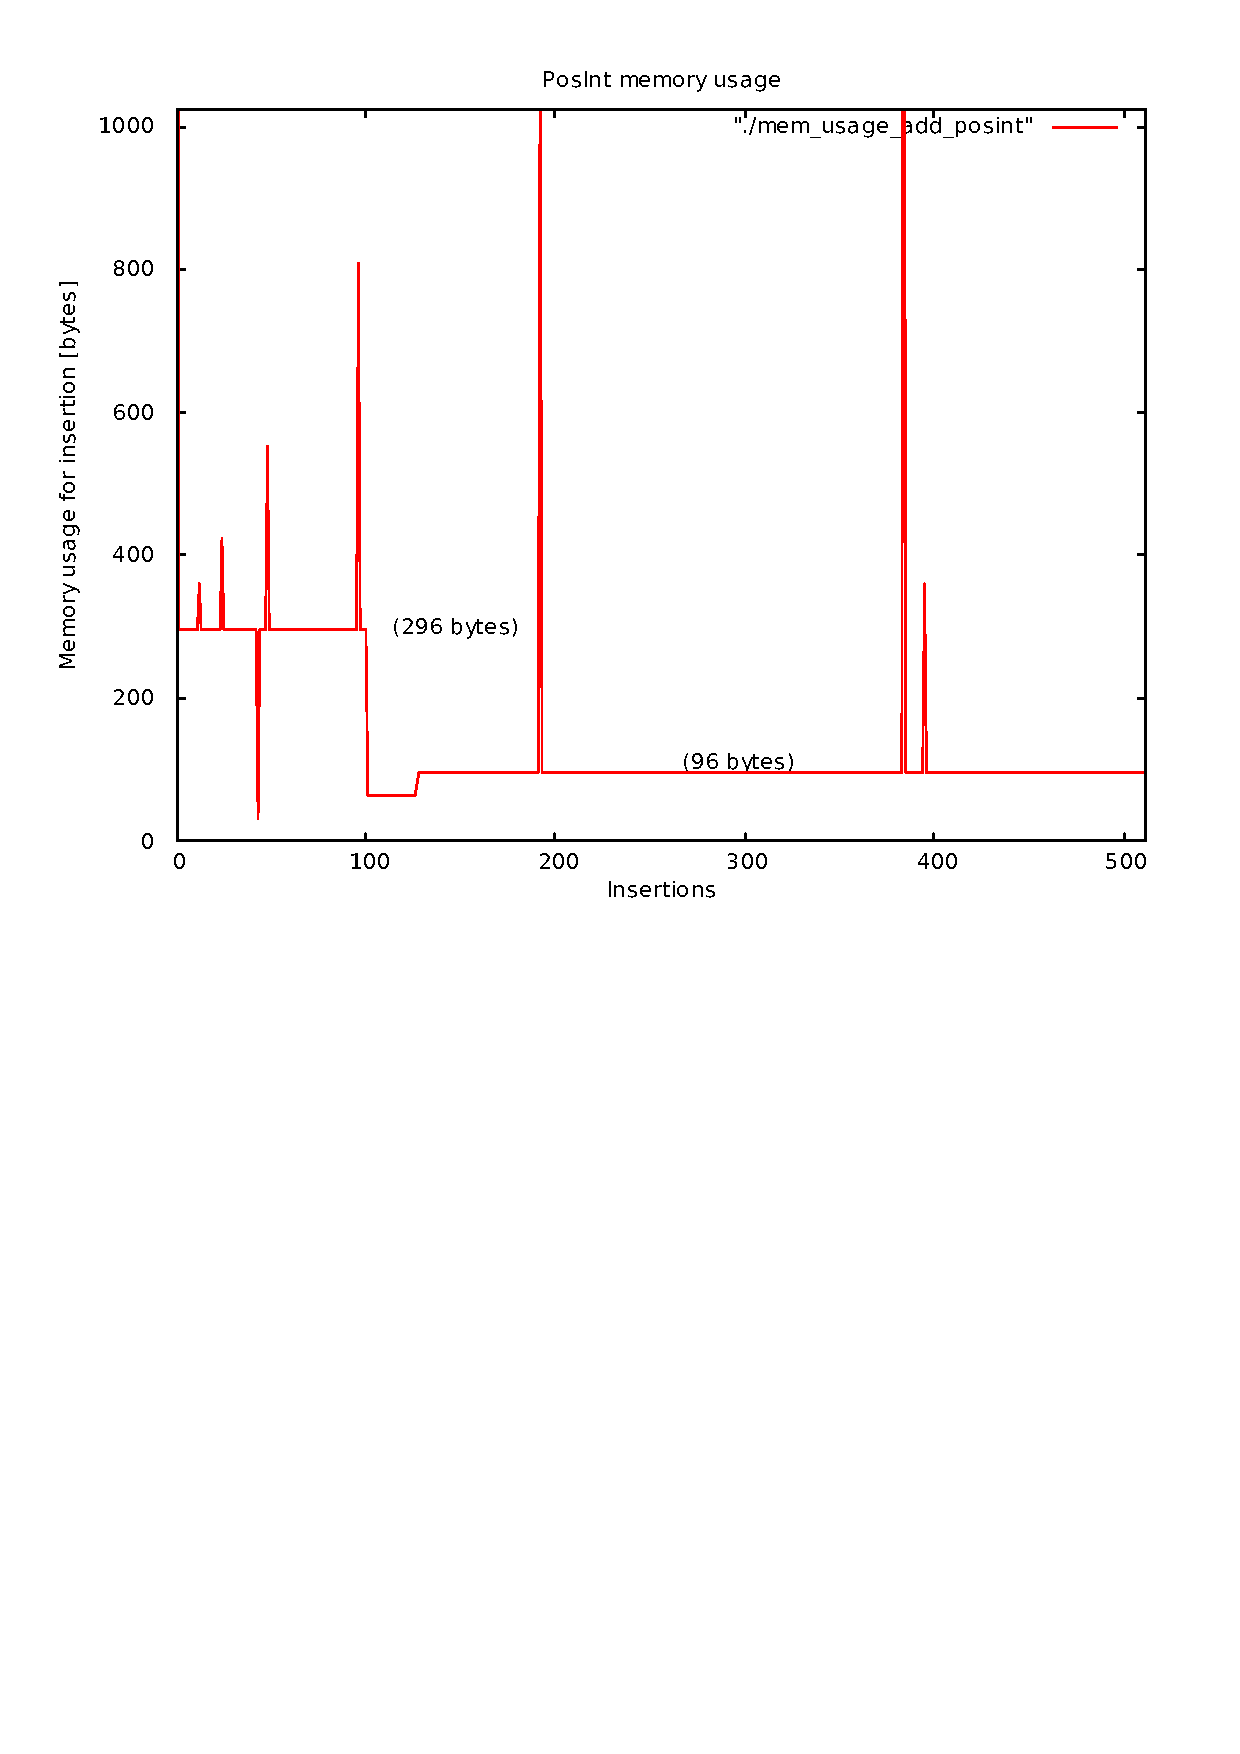
\includegraphics[width = 0.8\textwidth, trim = 0 15cm 0 0] {img/memoryConsumption_posint.pdf}
\caption{The memory usage}
\label{fig:memUsageInsertionPosInt}
\end{figure}


\subsubsection{Discussion}

Ideally, each insertion would take up the same amount of memory, but
figure \ref{fig:memUsageInsertionPosInt} suggests otherwise. The
very first insertion is shown to cost 49128 bytes. The excessive size
can be attributed to class loading, which is performed at the first
initialization of a given object. After the first insertion, the memory
usage for each inserted integer is 296 bytes, then dropping to 64
bytes after 100 insertions. At the 128th insertion, the memory usage
for each insertion increases to 96 bytes, and it stays at this level
for the rest of the insertions. It is, however, difficult to conclude
what causes these memory changes, at these exact points in time.

The spikes that are seen at insertion number 12, 24, 48, 96, 192 and
384 are related to the expansion of hash maps.

96 bytes for storing an integer is a significant memory overhead,
caused by storing the data in our Entry objects. It can be explained
by the many levels of wrapping of values into objects, that occurs
in EDMA. The diagram shown in figure \ref{fig:valueStorageOverhead}
shows the wrapping that occurs when storing an integer value in EDMA.

\begin{figure}[h!]
\centering
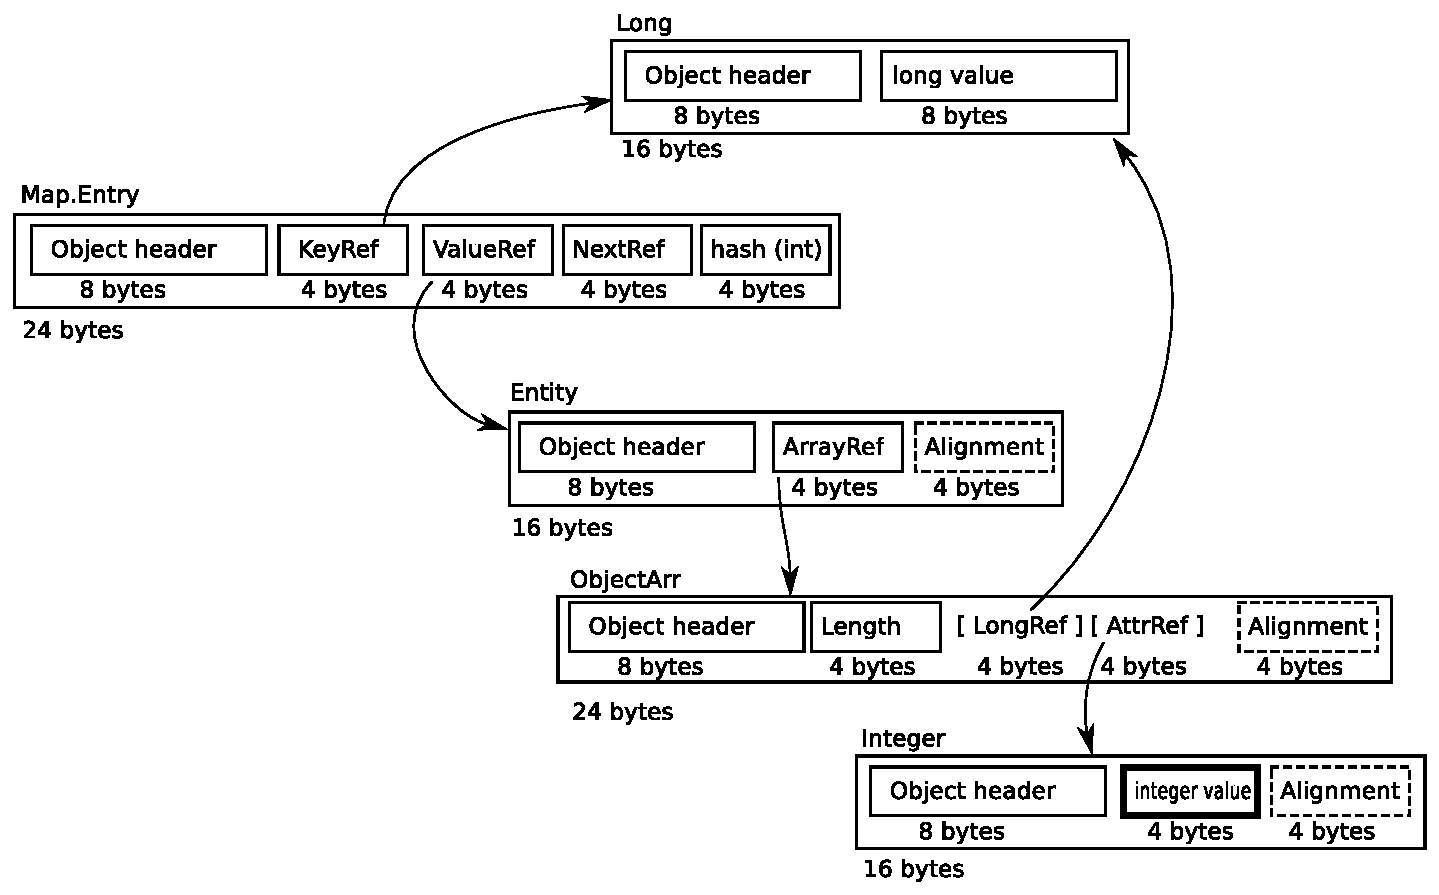
\includegraphics[width=\textwidth]{img/valueStorage.pdf}
\caption{This diagram shows the wrapping that occurs when storing data values in EDMA. A Map.Entry object holds a key reference and a value reference to the Entity object, wrapping the array containing the data value (the bold box).}
\label{fig:valueStorageOverhead}
\end{figure}

The diagram shows several contributions to the excessive memory use
-- object headers take up 8 or 16 bytes (on 32 bit and 64 bit platforms
respectively), and the JVM performs 8 byte alignment \cite{dieckmann1999study},
contributing to unnecessary allocation. This is further enhanced when
having many instances of small objects. The storage of the bold-boxed
integer in figure \ref{fig:valueStorageOverhead} adds up to a total
of 96 bytes, like the graph in figure \ref{fig:memUsageInsertionPosInt}
suggests.


\subsection{Data Insertion Response Time}

The response time for inserting data is measured in the following
procedure.
\begin{itemize}
\item Precondition: An empty data model instance must be started.
\item Flow of events:

\begin{enumerate}
\item Prepare an entity to insert.
\item Record the current time.
\item Insert the prepared entity.
\item Record the current time, and calculate the time difference.
\end{enumerate}
\end{itemize}
The reason for the entity value to be prepared before the time taking
starts, is that we want to measure only the response time of inserting
data -- not including creating the data values.


\subsubsection{Results}

Figure \ref{fig:insertionDvuResponse} shows the response time of
inserting entities. 

\begin{figure}[h!]
\centering
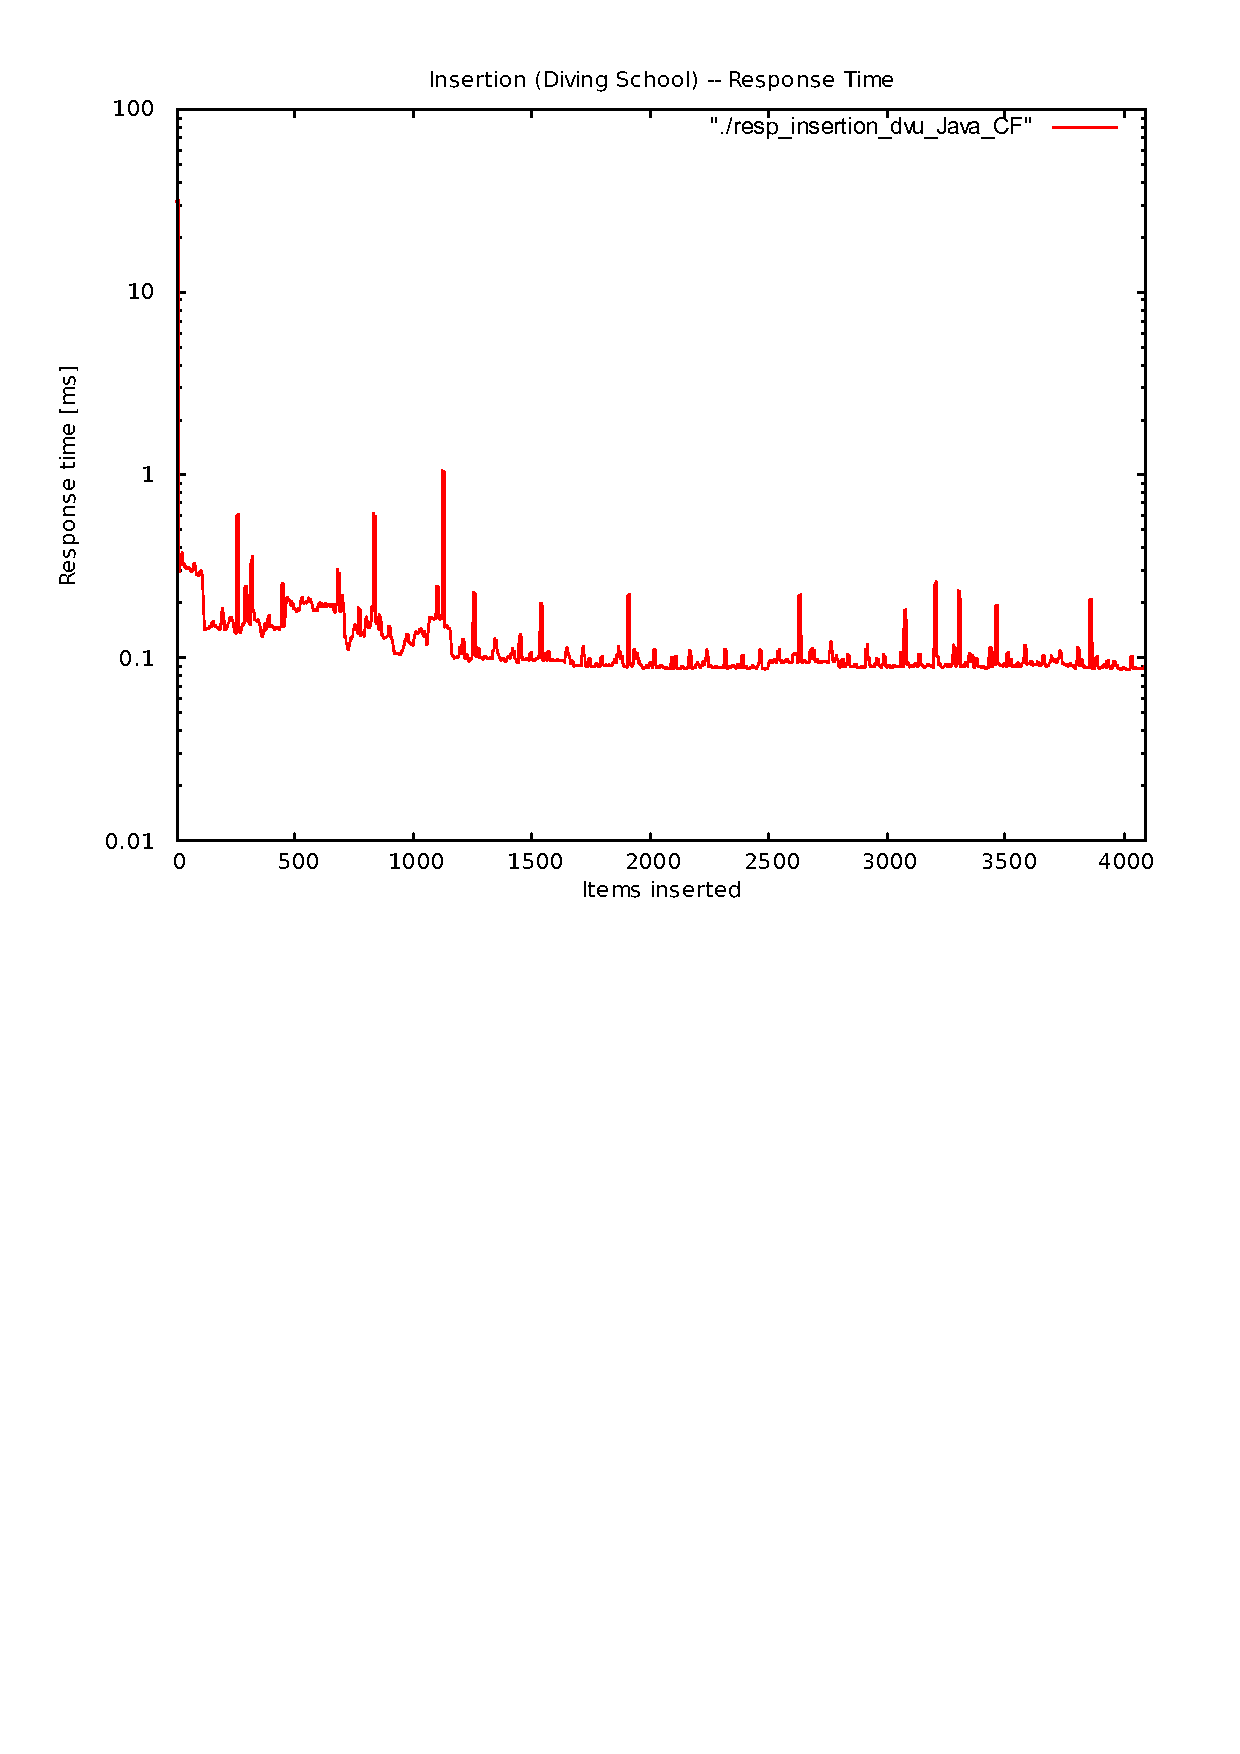
\includegraphics[width = 0.8\textwidth, trim = 0 15cm 0 1cm] {img/insertionDvuResponse.pdf}
\caption{This figure shows the response time of inserting new Person entities.}
\label{fig:insertionDvuResponse}
\end{figure}


\subsubsection{Discussion}

The response time for the very first insertion is rather high (31
ms), because it includes class loading. After classes have been loaded,
the response time drops to around 0.3 ms. After about 1200 insertions,
the response time finds a stable level at around 0.1 ms per insertion.


\subsection{Data Insertion Throughput}

In order to measure the throughput when inserting data, the following
procedure is executed.
\begin{itemize}
\item Precondition: An empty data model instance must be started.
\item Flow of events:

\begin{enumerate}
\item Create a number of worker threads, with the job of inserting a certain
number of entities.
\item Record the current time.
\item Start all the worker threads.
\item Join all the worker threads (wait for their finish.)
\item Record the current time, calculate the time difference and throughput.
\item Clear the data model instance -- remove all entities.
\item Increase the number of worker threads, and go back to step 1.
\end{enumerate}
\end{itemize}
The test has been run, inserting 32768 Person entities, divided between
the number of worker threads. 


\subsubsection{Results}

Figure \ref{fig:insertionDvuThroughput} shows the insertion throughput,
varied by the number of concurrent worker threads. It is seen that
the single-threaded throughput measure is at the lowest, running at
12 insertions/ms. Running with two threads increases the throughput
to 22 insertions/ms, and with four threads the throughput is 44. Running
with up to 100 threads, the throughput varies between 46 and 57 insertions/ms.

\begin{figure}[h!]
\centering
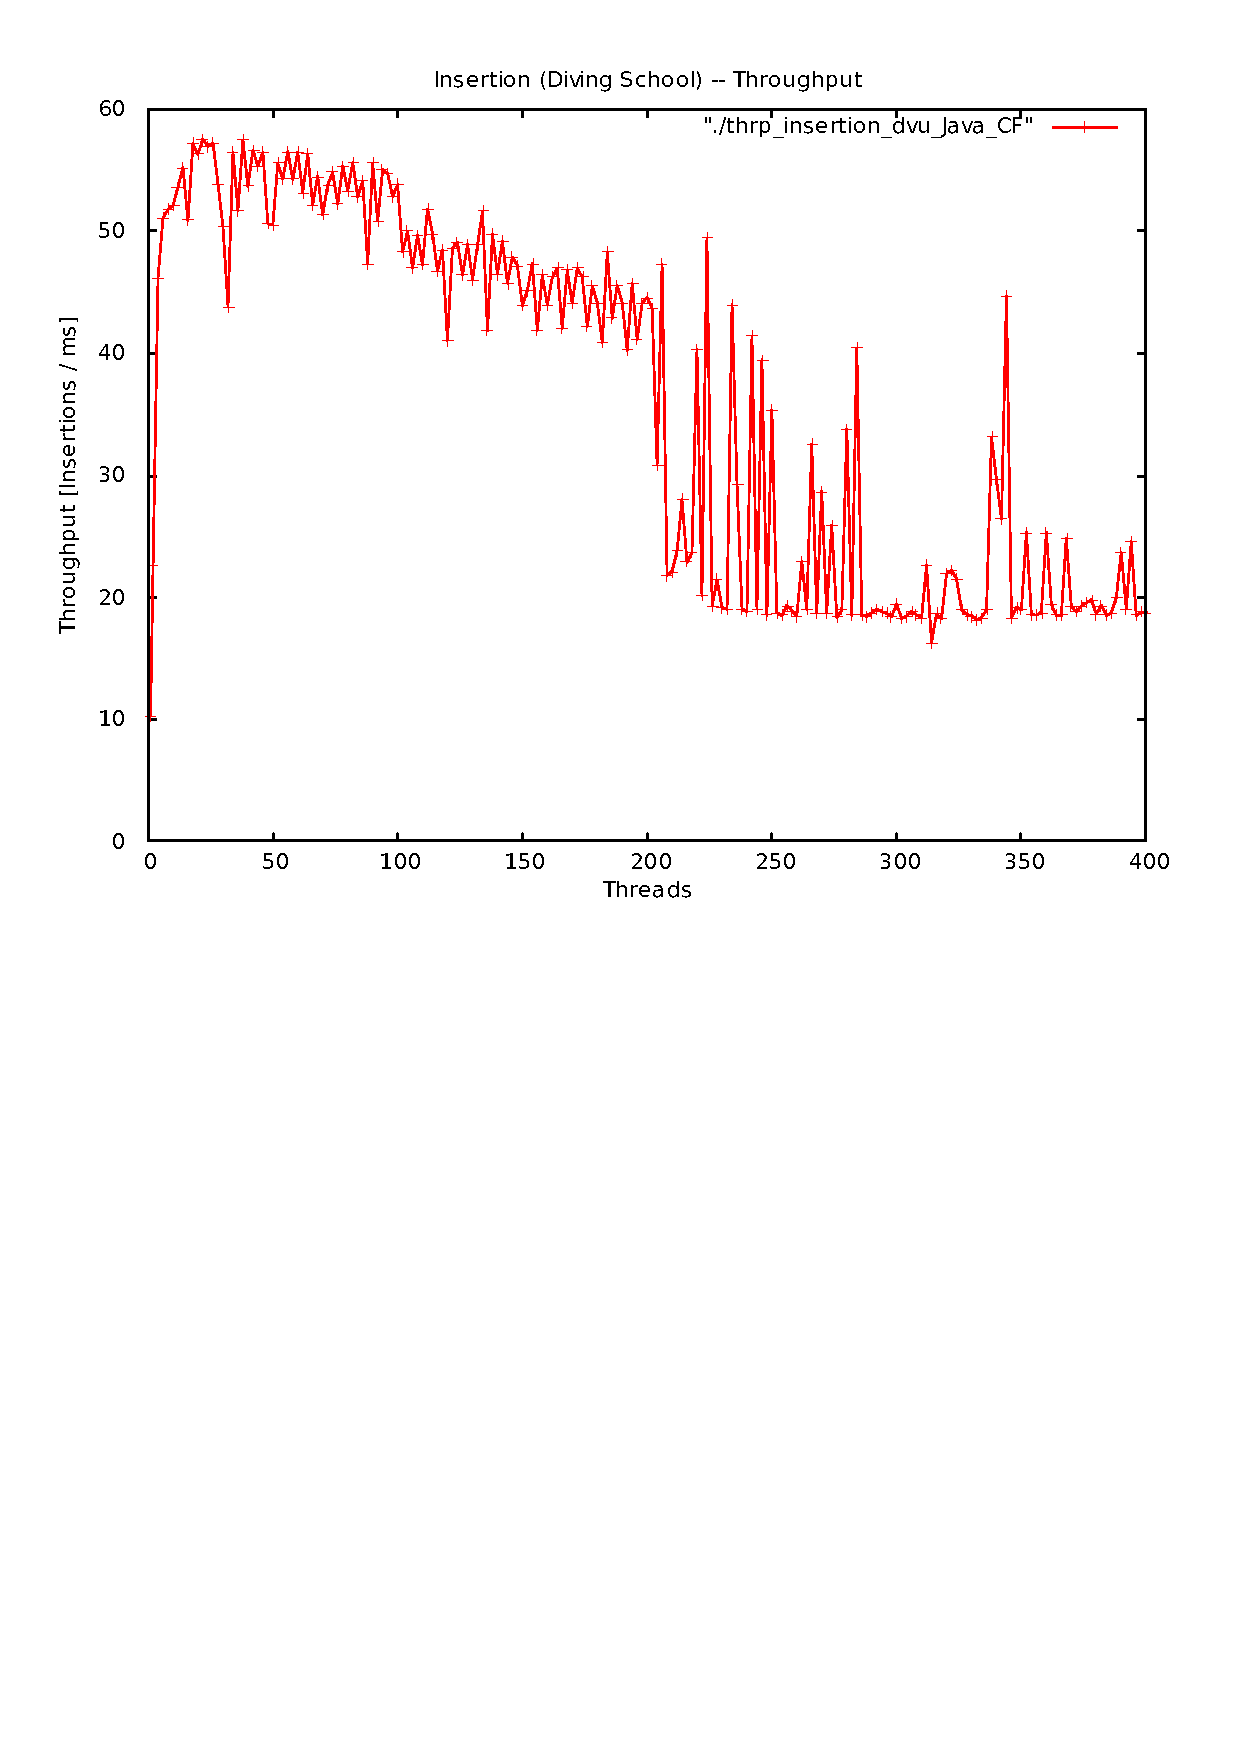
\includegraphics[width = 0.8\textwidth, trim = 0 15cm 0 1cm] {img/insertionDvuThroughput.pdf}
\caption{This figure shows the throughput (insertions per ms), as a function of the number of concurrent threads.}
\label{fig:insertionDvuThroughput}
\end{figure}Running with more than 100 threads shows a decreasing tendency in
the throughput. This might be because either the execution buffer,
or the persistence buffer, is occasionally full -- they are both set
to a maximum size of 100, in the current implementation. Using 200
or more threads, shows a drastic decrease in the throughput, because
both of the buffers are filled, causing blocking of the worker threads.
Here, the throughput falls to about the same level as when using 2
threads (around 20 insertions/ms.)


\subsubsection{Discussion}

It is not obvious, why the graph looks like it does. Going from one
to two threads doubles the throughput as expected, but we wouldn't
expect much more throughput by using more than two threads. A plausible
explanation would be the overhead that is involved in changing the
state of threads, by calling wait and notify. The two running units
in our two step pipeline utilize two synchronized buffers, causing
many calls to wait and notify. Using two threads, we keep the slowest
of the two execution units (often the persistence unit) busy However,
when using 3 or more threads, both the executor and the persist are
kept busy most of the time, causing fewer thread state changes. This
could explain why extra performance is gained using more than 2 threads.


\subsection{Data Retrieval Response Time}

In order to measure the response time of retrieving data, we insert
a large number of Person entities into a running data model instance.
We then search for persons, that we know have been put into the data
model instance.
\begin{itemize}
\item Precondition: A data model instance has been started, and 10000 Person
entities has been inserted. The first and last name of each Person
entity has additionally been stored in a list.
\item Flow of events:

\begin{enumerate}
\item Get a random first name and last name from the list of inserted names.
\item Record the current time.
\item Run the view that retrieves Persons from the chosen first name and
last name.
\item Record the current time, calculate the time difference, and go back
to step 1.
\end{enumerate}
\end{itemize}

\subsubsection{Results}

The response time when using two different indexes (a compare index
and an equals index) is shown in figure \ref{fig:retrievalDvuResponse}.

\begin{figure}[h!]
\centering
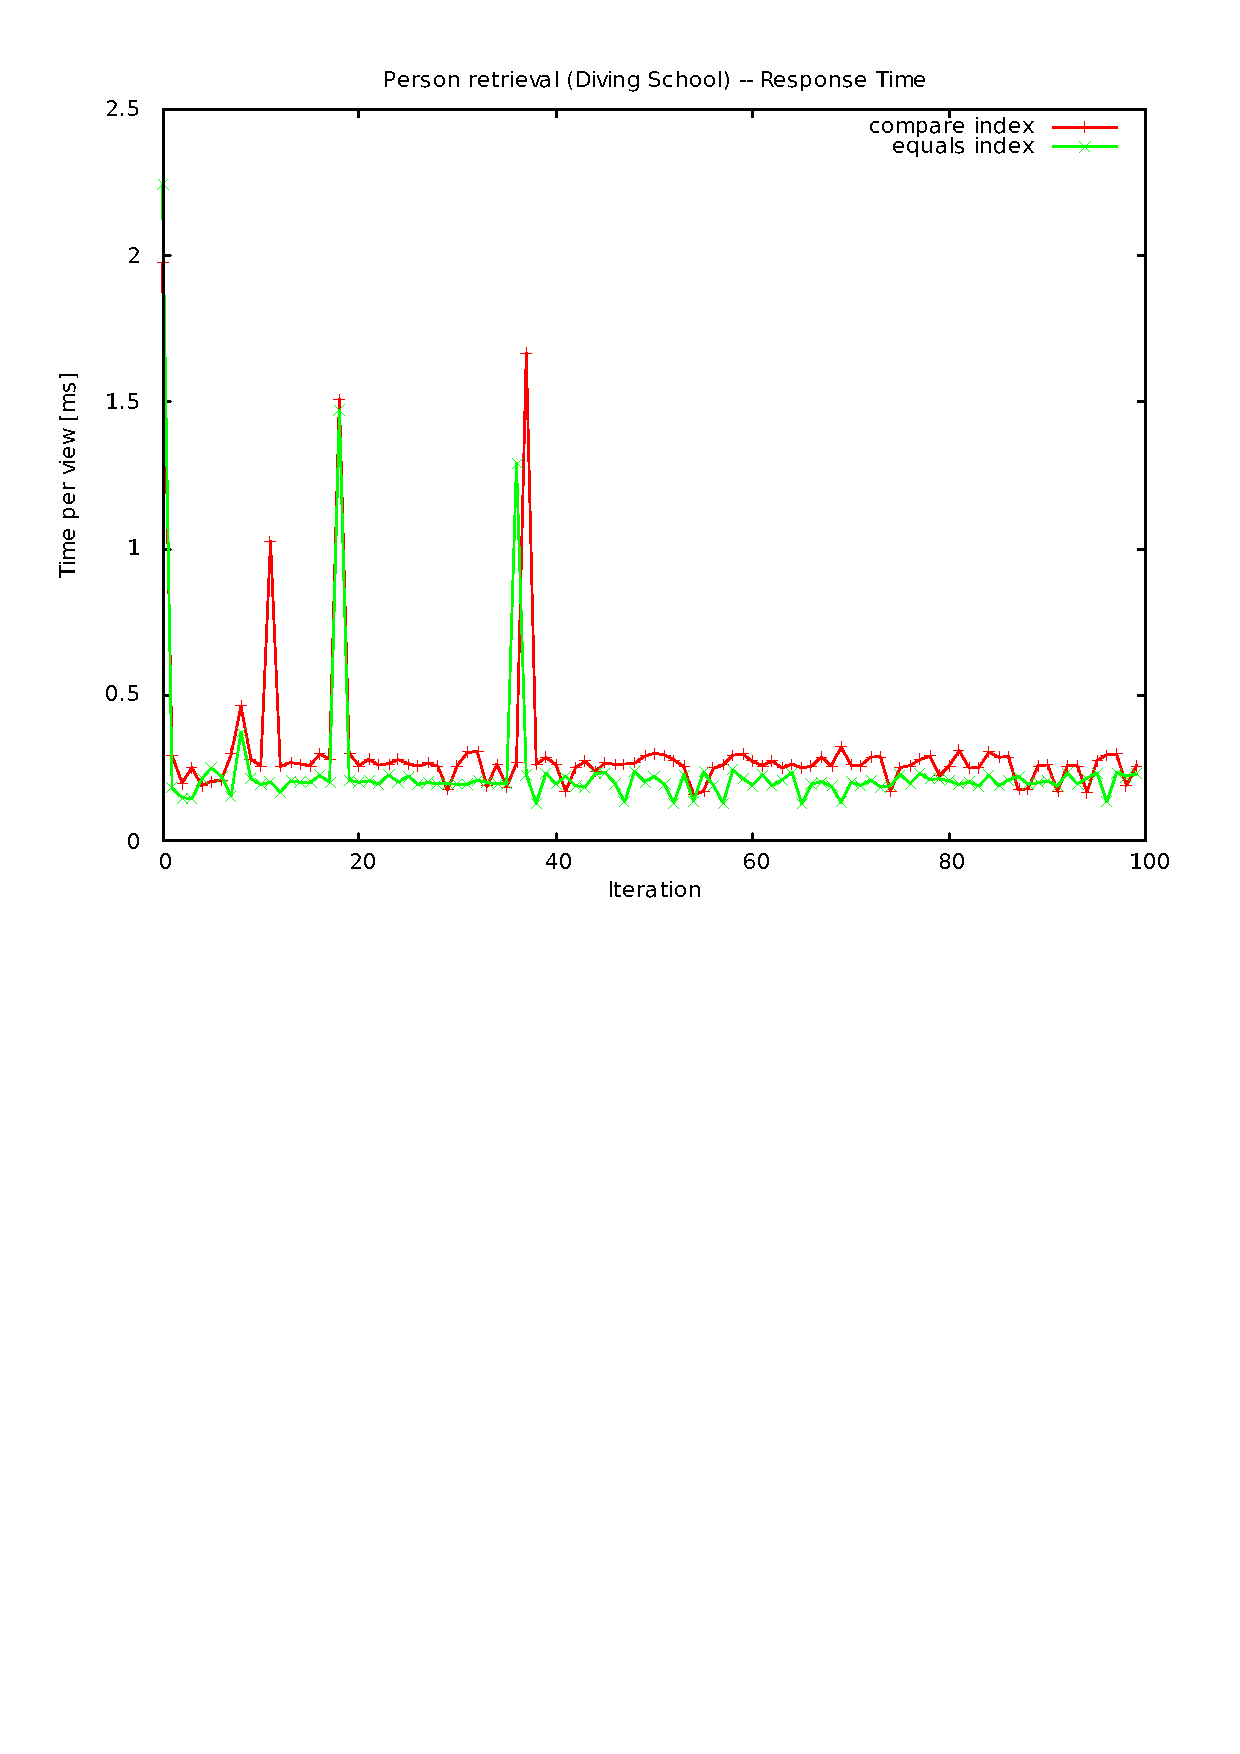
\includegraphics[width = 0.8\textwidth, trim = 0 15cm 0 1cm]{img/retrievalDvuResponse.pdf}
\caption{This figure shows the response time for searching for Persons with a randomly chosen name (guaranteed to find at least 1), using two different types of indexes.}
\label{fig:retrievalDvuResponse}
\end{figure}


\subsubsection{Discussion}

The response time lies around 0.16 ms to 0.30 ms when using the compare
index (which is based on a tree map), while the equals index (based
on a hash map) is slightly faster, ranging from 0.12 ms to 0.22 ms.


\subsection{Data Retrieval Throughput}

Measuring the throughput of retrieving data is done by creating a
variable amount of worker threads, each retrieving a Person from the
first name and last name.
\begin{itemize}
\item Preconditions: A data model instance is started, and 100.000 Person
entities has been inserted. The first and last name of each Person
entity has additionally been stored in a list.
\item Flow of events:

\begin{enumerate}
\item Run garbage collection and finalization.
\item Create a number of worker threads, each with the task of retrieving
a person from a first name and last name.
\item Record the current time.
\item Start all the worker threads.
\item Join all the worker threads.
\item Record the current time.
\item Calculate the throughput, as the number of views executed per millisecond.
\item Increase the number of worker threads, and go back to step 1.
\end{enumerate}
\end{itemize}
The worker threads together execute a total of one million views.


\subsubsection{Results}

The results for the throughput measuring can be seen in figure \ref{fig:retrievalDvuThroughput}.

\begin{figure}[h!]
\centering
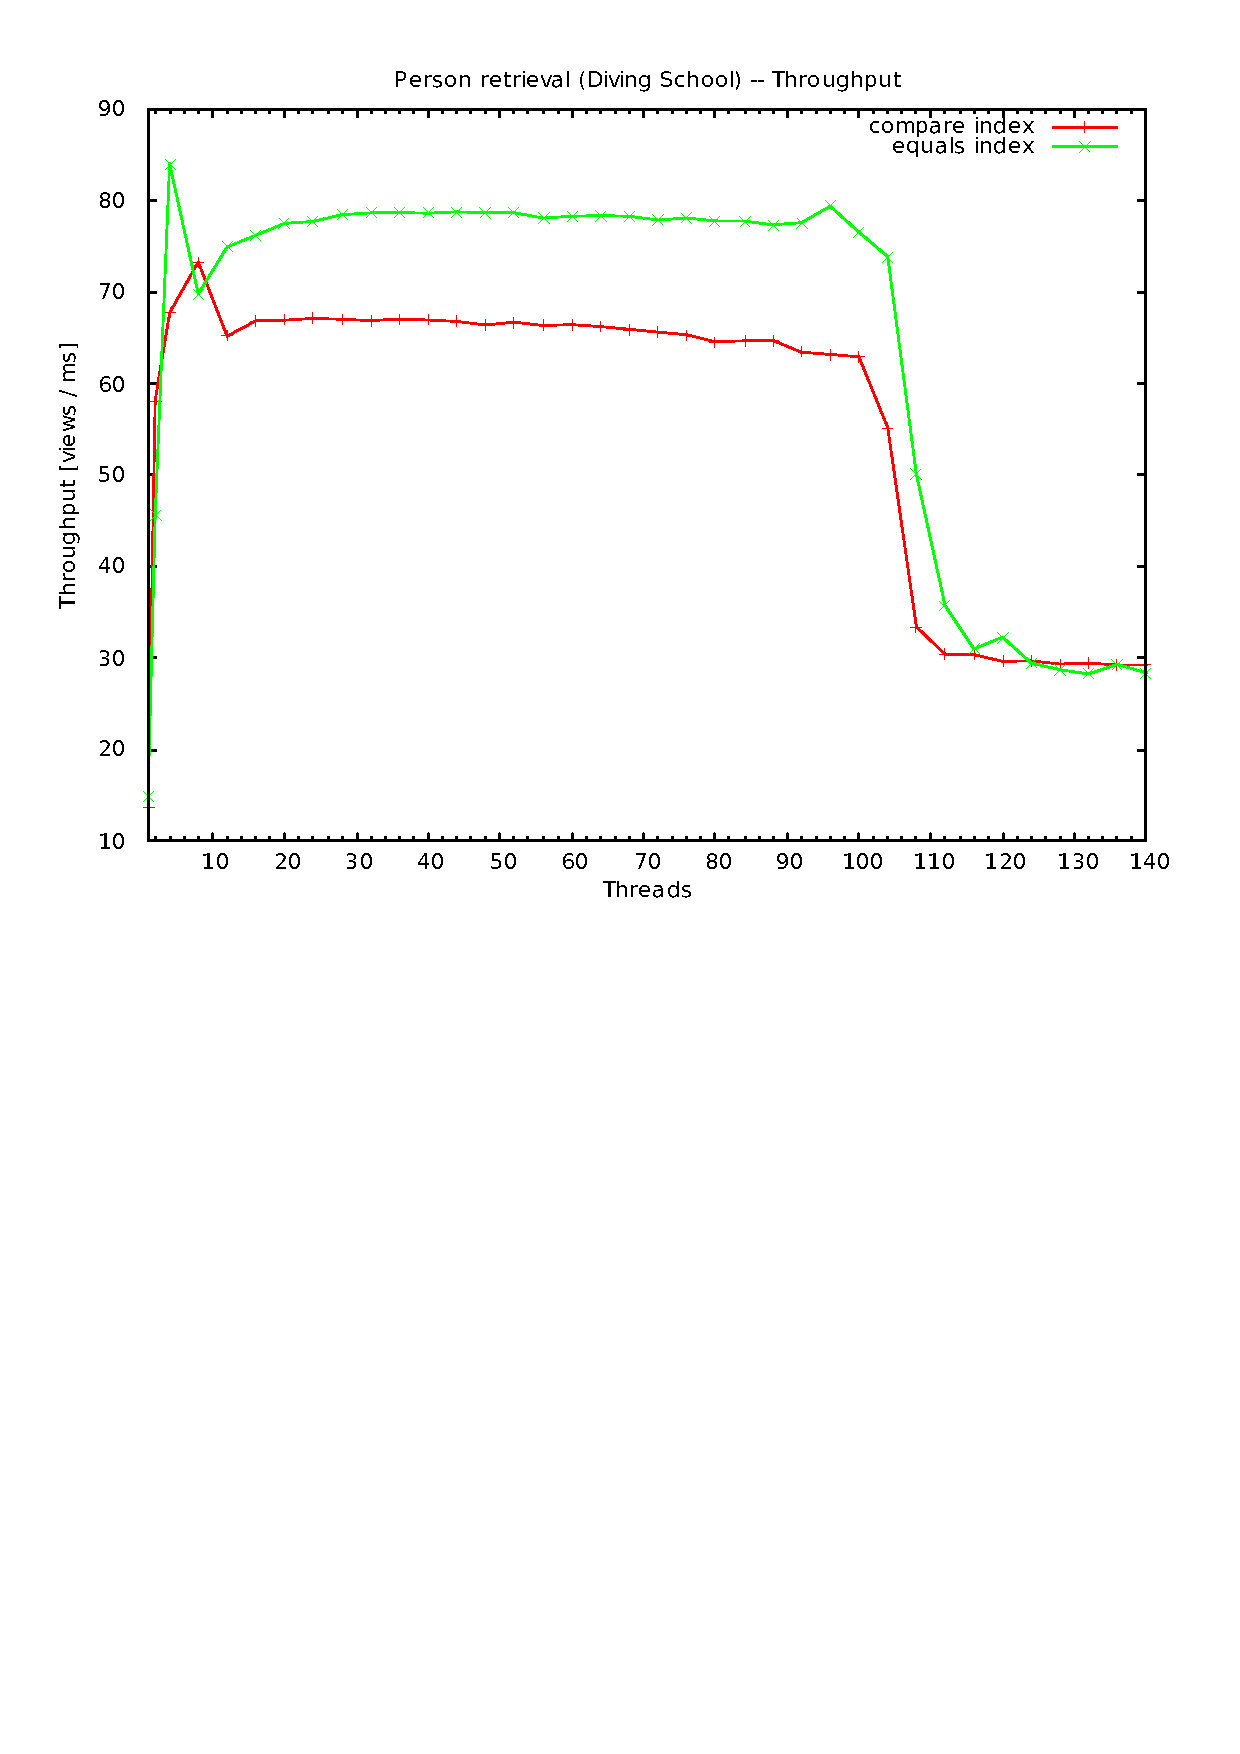
\includegraphics[width = 0.8\textwidth, trim = 0 15cm 0 1cm]{img/retrievalDvuThroughput.pdf}
\caption{This figure shows the throughput of having a number of threads searching for Persons with randomly chosen names (guaranteed at least one hit). Two different kinds of indexes are used, a compare index and an equals index.}
\label{fig:retrievalDvuThroughput}
\end{figure}

The x-axis shows the number of concurrent threads to perform the views,
and the y-axis shows the calculated number of persons that was retrieved
per millisecond.

Running with one thread gives a throughput of 13.75 views / ms with
the compare index, and 14.8 with the equal index. Increasing the number
of threads to 2 gives a compare index throughput of 58 views / ms,
while the equals index is 45 views / ms. The throughput stabilizes
at around 78 views / ms for the equals index, and 67 views / ms for
the compare index, as long as there are less than 100 worker threads.
Using more than 100 threads, the throughput drops to about 30 views
/ ms.


\subsubsection{Discussion}

The results show, as expected, that the equals index has a higher
throughput value than the compare index, and that running with multiple
threads has a great impact, compared to running with only one thread.
However, when the number of threads is higher than the size of the
execution buffer (here 100), the throughput drops to around 30 views
/ ms.


\subsection{Interleaved Actions and Views}

In order to see how the number of actions affects the total throughput,
when running interleaved actions and views, we run the following procedure.
\begin{itemize}
\item Precondition: A data model instance has been started, and 100.000
Person entities has been inserted.
\item Flow of events:

\begin{enumerate}
\item $p_{action}$, the probability of running an action instead of a view,
is set to 0.
\item While \emph{$p_{action}\leq1$}

\begin{enumerate}
\item 50 worker threads are created, with the task of running either an
action or a view in each iteration, depending on $p_{action}$.
\item The current time is recorded.
\item All the worker threads are started.
\item All the worker threads are joined.
\item The current time is recorded.
\item The total number of actions and views are determined.
\item The total throughput, the view throughput and the action throughput
is calculated.
\item $p_{action}$ is increased by 0.02.
\end{enumerate}
\end{enumerate}
\end{itemize}

\subsubsection{Results}

The result of running interleaved actions and views can be seen in
figure \ref{fig:interleavedActionsAndViewsThroughput}.

\begin{figure}[h!]
\centering
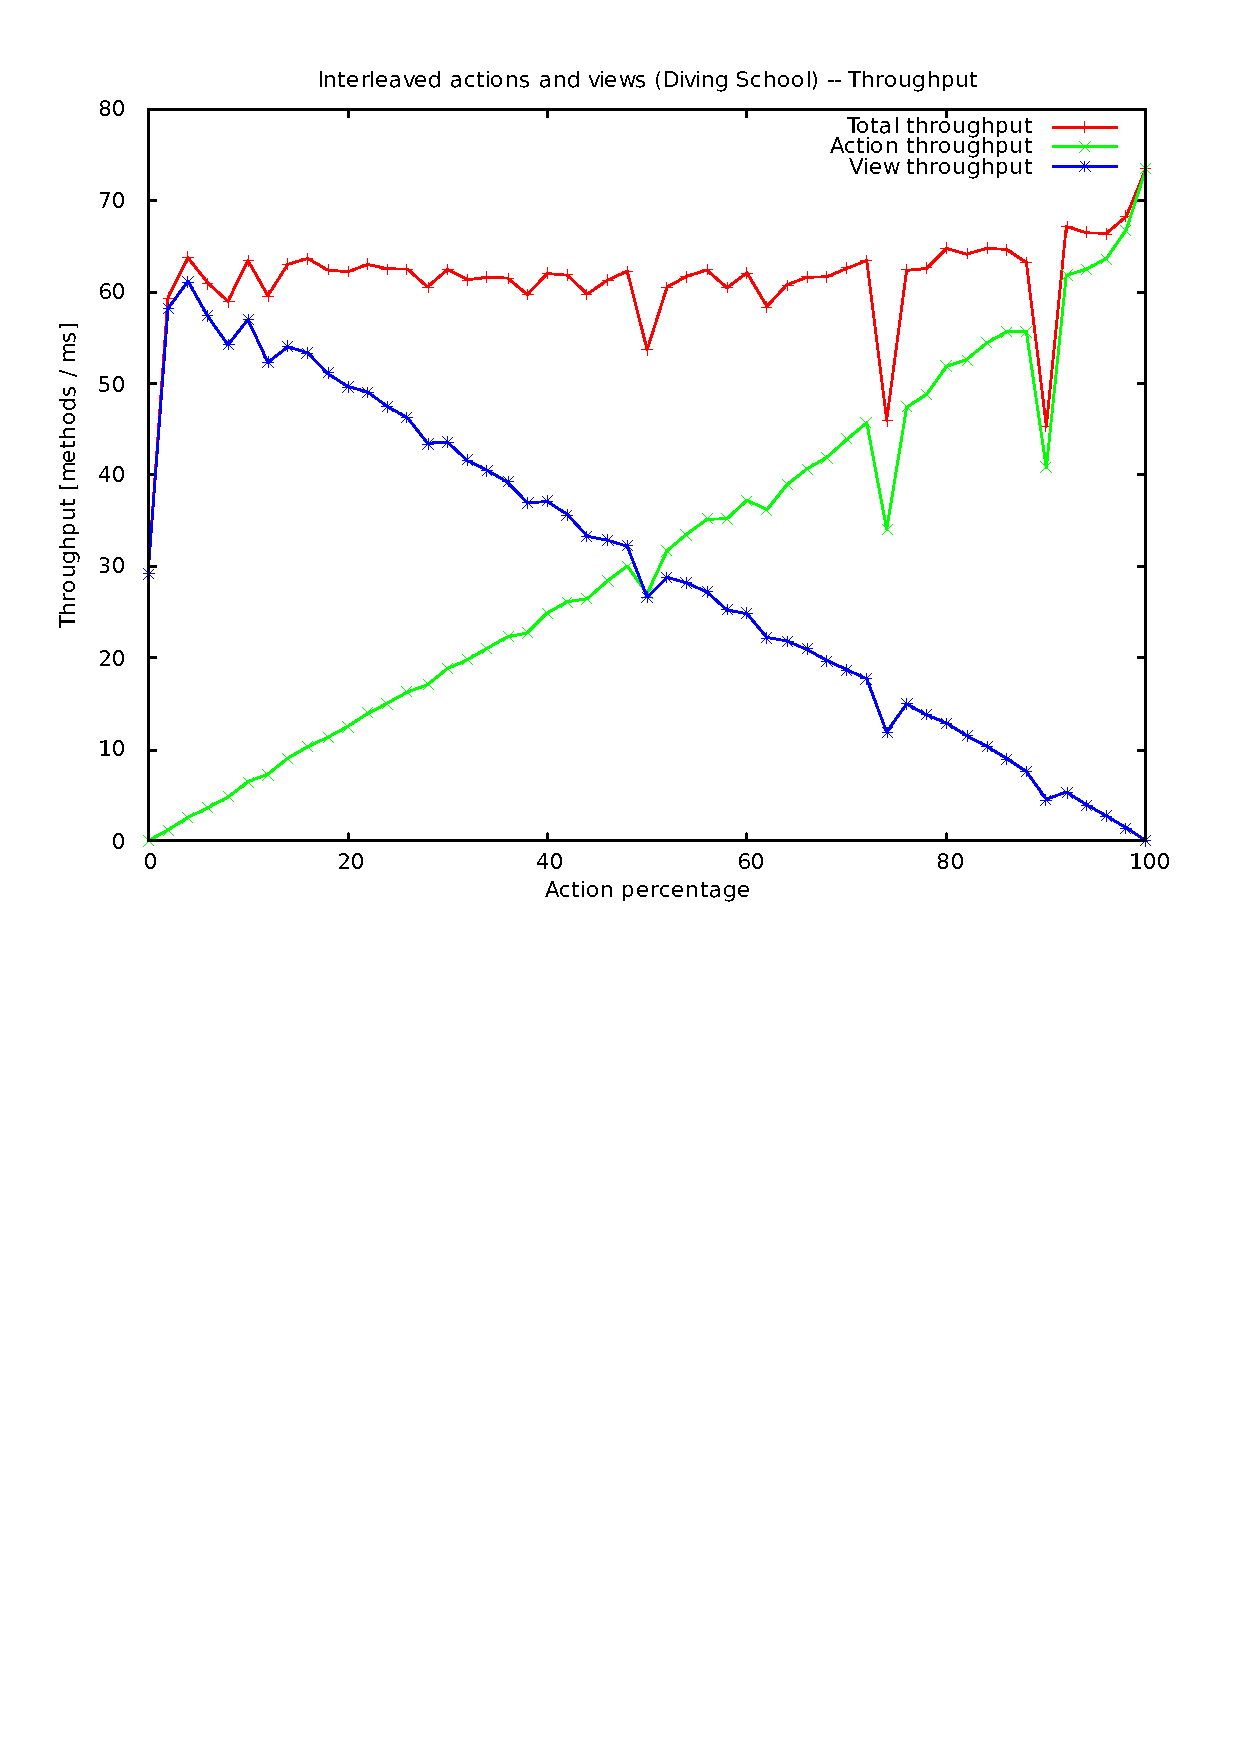
\includegraphics[width=0.8\textwidth, trim=0 15cm 0 1cm] {img/interleavedActionsAndViewsThroughput.pdf}
\caption{This graph shows the result of running interleaved actions and views. 50 worker threads are set to run concurrently. Each worker thread runs for a number of iterations, where each iteration can run either an action or a view, determined by the probability factor (the x-axis). The throughput is shown on the y-axis.}
\label{fig:interleavedActionsAndViewsThroughput}
\end{figure}


\subsubsection{Discussion}

The graph shown in figure \ref{fig:interleavedActionsAndViewsThroughput}
shows that the total throughput remains constant, even if the probability
of running actions increases. The action throughput seems almost directly
inverse to the view throughput, which is contrary to our expectations.
Since our runtime system is able to run multiple views concurrently,
but not actions, we would expect a dropping total throughput, when
increasing the number of actions run.


\subsection{Scalability}

Scalability denotes the possibilities of adding workload to the system.
Andre B. Bondi of Bell Labs proposes definitions of 6 different scalability
aspects in \cite{bondi2000characteristics}. According to Bondi, there
are at least the following aspects of scalability:
\begin{lyxlist}{00.00.0000}
\item [{Load~Scalability}] -- describes how well a system is able to function
gracefully at light, moderate or heavy load, i.e. mostly considering
variance in the number of users.
\item [{Space~Scalability}] -- describes how the memory requirements changes,
as the amount of data handled by a system changes. The system can
be considered spatially scalable, if the memory usage grows sublinearly
with the number of data items in question.
\item [{Space-Time~Scalability}] -- describes the ability for a system
to function gracefully, when the amount of data changes by orders
of magnitude.
\item [{Structural~Scalability}] -- describes whether a system uses data
structures or algorithms that naturally limit the amount of data that
can be contained or dealt with.
\item [{Distance~Scalability}] -- the ability for a system to operate
over short as well as long distances (considering issues such as reliability
at drop-outs, timing issues, noise, etc.)
\item [{Speed/Distance~Scalability}] -- the ability for a system to operate
at high speed over short as well as long distances.
\end{lyxlist}
Throughout the project, some of these scalability aspects has been
prioritized higher than others. In the beginning of developing the
EDMA system, although not formally stated anywhere, it was the thought
that it should be able to serve small businesses with ``thousands''
of users (<10000). 


\subsubsection{Load Scalability}

The load scalability mainly depends on the execution of actions and
views, together with the persistence. According to Bondi, load scalability
can be improved by not having unproductive execution cycles in the
program, avoiding busy waiting, and allow parallel execution where
possible. As explained in the section about the transaction execution,
EDMA is able to execute multiple views at the same time. However,
only one action can be executed at the time, which puts a boundary
on the load scalability. However, even if only one action can be executed
at the time, heavy load will have the system continue gracefully,
until a certain degree, determined by the maximum size of the execution
buffer and the persistence buffer. When these are both filled, throughput
decreases drastically, as shown in the test of data insertion throughput.


\subsubsection{Space Scalability}

The space scalability depends on how data is stored in the runtime
system, and how it is persisted on the disk.

In the runtime system, data is held in the memory, in the kind stores.
The kind stores hold all data entities in maps, with an ID as key
(as a long), and an Entity object as value. The Entity contains an
Object array, holding the actual attribute values. However, the value
domain system uses instance control, guaranteeing that two equal values
will only be instantiated once in the memory. Therefore, the entities
that are kept by the kind store may reuse each others' values. However,
the kind store still has to hold separate Entity objects for each
entity, making it linearly growing with the amount of data. This makes
the system less scalable as seen from the spatial aspect. The upper
bound for the amount of data is decided by the choice of either using
Java maps, or maps from the JDBM3 library (the user chooses this upon
instantiation of the data model.) If the former is used, the upper
bound is determined by the amount of RAM that is available to the
Java Virtual Machine. If the latter is used, the upper bound is determined
by the disk size.


\subsubsection{Space-Time scalability}

With respect to data search, EDMA uses tree maps for compare-indexes
and hash maps for equal-indexes, making it efficient. If the user
instead uses a custom made filter to search for data of a certain
kind, data is traversed linearly, hurting the space-time scalability.
Therefore, the user should be encouraged to use indexes as much as
possible, and applying custom filters as late in the search process
as possible.


\subsubsection{Structural scalability}

Naturally, there are limits for how much data can be stored. If regular
Java maps are used for storing the runtime data, the amount of RAM
accessible is a limit for the data amount, and the file system is
a limit for the log file size. 

From the user's point of view, some aspects of the EDMA system are
structurally scalable, while others are not. There are some logical
problems in changing a data model, after it has been taken into use
-- for example:
\begin{itemize}
\item If a kind is removed, what should be done when the data model tries
to load the log file, where the kind existed?
\item If non-optional attributes are added to a kind, or a new kind with
non-optional attributes is added, what should be the values of the
new attributes? When the log file is loaded, how can kind entities
be created, if there are no stored values for the newly added attributes?
\item What should be done if a kind or an attribute is renamed?
\end{itemize}
Some of these problems can be solved by having more interaction with
the user -- for example, in the case of renaming an element, the user
could explicitly tell EDMA the old name and the new name of the element,
upon instantiation. In the case of newly added attributes, the user
could either manually or automatically supply the missing data, possibly
adding null-data or temporary ``dummy'' data (e.g. 00000000 for
phone number.)

In this project, we haven't taken into account that the user should
be able to change the data model after it has been taken into use.
However, because of it's structure, the user is able to make the following
changes to a data model, after it has been taken into use (i.e. data
has been stored in the log file):
\begin{itemize}
\item Adding kinds (after the last kind in the data model in the data model
definition)
\item Adding optional attributes to kinds
\item Adding relations (after the last relation in the data model definition)
\item Adding actions and views
\item Adding indexes to existing kinds and relations
\end{itemize}
The reason to only be able to be added ``in the end'', is that the
runtime system uses the sequential order of the kind (0, 1, 2, ...)
in the definition file, rather than the kind name. Adding a kind in
the top, will therefore push all the other kinds one step forward,
which will invalidate the log file. 

The following is not possible without substantial changes to the system:
\begin{itemize}
\item Removing or renaming kinds, attributes, relations, actions or views
(renaming or removing actions or views does not break anything in
the runtime system directly, but will break the user's code)
\item Adding non-optional attributes to kinds\end{itemize}





\printnomenclature{}

\bibliographystyle{plain}
\addcontentsline{toc}{section}{\refname}\nocite{*}
\bibliography{reportBib}

\end{document}
